\documentclass[11pt]{article}
\usepackage{report}


\usepackage{silence}
\WarningFilter{latex}{Text page 83 contains only floats}

\title{Solid State Physics \\ Notes}
\author{Jesper Vesterberg (jeve0010@student.umu.se)}

\date{\today}

\begin{document}
\begin{titlepage}
  \maketitle
  \thispagestyle{fancy}
  \lhead{
    Department of physics\\
    Umeå Universitet
  }
  \rhead{\today}
  \begin{abstract}
		Collected notes of the whole course, base primarly on the course material (i.e.\ hook and halls book ``solid state physics'')
  \end{abstract}
	\cfoot{Solid State Physics}
\end{titlepage}
\lhead{\theauthor}
\rhead{\thetitle\\\today}
\cfoot{\thepage}

\tableofcontents
\newpage

\section{Crystal Structure}
\subsection{Elementary Crystallography}
\subsubsection{The crystal lattice}
The crystal lattice is a way to describe crystal structures. We can take for example graphite as showed in figure~\ref{fig:graphite}. In order to create the lattice we take a point in the structure, lets call it $O$, then we need to find all identical positions within the structure.

\begin{figure}[H]
	\centering
	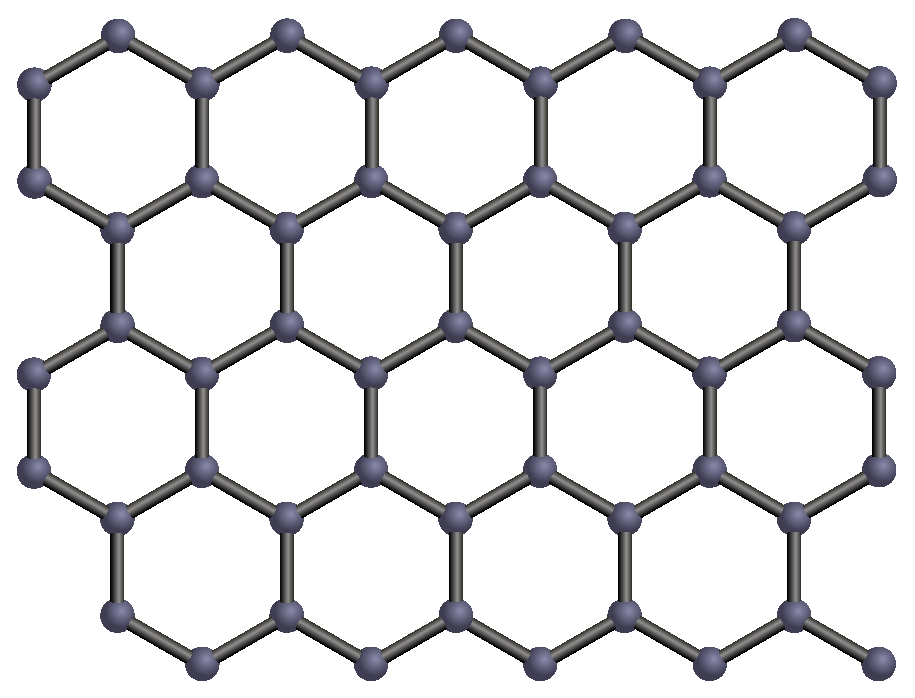
\includegraphics[width=0.8\textwidth]{graphite}
	\caption{Graphite lattice}
	\label{fig:graphite}
\end{figure}

\newpage
This choosing of $O$ and identification of identical position within the structure has been done in figure~\ref{fig:graphite-lattice}. Using this lattice which is highlighted in the dotted lines we see we have atoms on all lattice points except the atoms circled in yellow. This actually just fine, this is because we define all atoms related to lattice point through something called the basis, which we will look at in section~\ref{sec:basis}, this means that the crystal lattice do not have to coincide with any atom at all. Using the vectors $\mathbf{a}$ and $\mathbf{b}$ here we can define a vector which uniquely defines a point in the lattice relative $O$
\begin{equation}
	\mathbf{r}_{uv }= u\mathbf{a} + v\mathbf{v}
	\label{eq:crystal-lattice}
\end{equation}
All points defined through this equation are together called the \textbf{crystal lattice}. An important thing of this lattice is that it possesses \textbf{translational invariance}, which basically means that no matter from what lattice point you're looking at, the structure and environment looks precisely the same. For this to hold we need to presume that the lattice is practically infinite, which is something that is generally true. 

\begin{figure}[H]
	\centering
	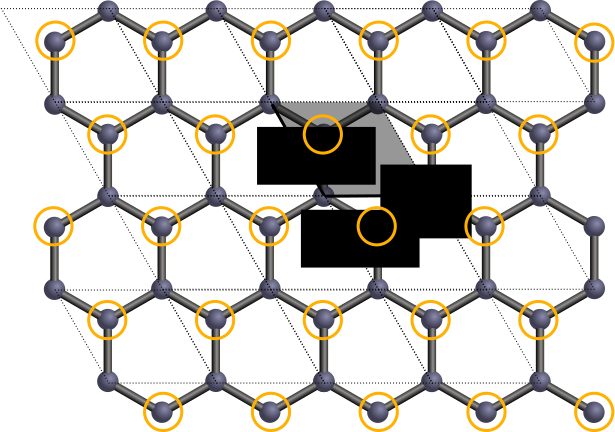
\includegraphics[width=0.8\textwidth]{graphite-lattice}
	\caption{Graphite structure}
	\label{fig:graphite-lattice}
\end{figure}

In three dimension this lattice general arguments extends but the vector that represents all positions in the lattice get an extra term as usual
\begin{equation}
	\mathbf{r}_{uvw} = u\mathbf{a} + v\mathbf{b} + w\mathbf{c}
	\label{eq:crystal-lattice-3d}
\end{equation}
and instead of getting an area as covered in grey by $\mathbf{a}$ and $\mathbf{b}$ in figure~\ref{fig:graphite-lattice}, we get a volume, a volume we call the \textbf{unit cell}.

\subsubsection{lattice symmetries}
The lattice symmetries are usually important when looking at the property of a certain solid. In turns out the available possibilities are quite limited too. We lattices such as the \textbf{rectangular lattice}, \textbf{rhombic lattice} and the \textbf{centred rectangular lattice}. Look in the book for further explanation.

\subsubsection{The basis}\label{sec:basis}
The basis is what we use to define a position of a particular atom within a lattice. For our example in figure~\ref{fig:graphite-lattice} we have vector 
\begin{equation}
	\mathbf{r}_b = \frac{2}{3}\mathbf{a} + \frac{1}{3} \mathbf{b}
	\label{eq:basis}
\end{equation}
that defines the position of the yellow circled atom from a lattice point. But the basis also describes the type of atom, thus we end up with the basis 
\begin{equation}
	C(0,0),C(\frac{2}{3}, \frac{1}{3})
\end{equation}
where the first $C$ defines the atom at the lattice point, and the second the other atom which was on on the lattice ($C$ specifies that it is a carbon atom).
Likewise for a three dimensional structure we just add one simple term for the position. 

Taking the symmetry of the basis as well as the crystal lattice, we can sort a crystal into on of the 32 possible \textbf{point symmetry groups} or \textbf{crystal classes} and one of the 230 possible \textbf{space symmetry groups}.

\subsubsection{Crystal planes and directions}
Imagine we have a three dimensional rectangular lattice(incidently called a cubical lattice) that we depict in two dimensions as we have done in figure~\ref{fig:lattice-planes}. We can then define a multitude of planes that goes through multiple lattice points. In two dimension in looks simply like lines, but if we stretch that out in three dimensions we can easily see the planes, which is more clearly depicted in figure~\ref{fig:lattice-planes-3d}.
\begin{figure}[H]
	\centering
	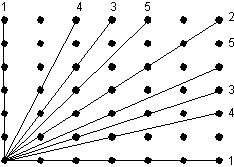
\includegraphics[width=0.8\textwidth]{lattice-planes}
	\caption{Some lattice planes in the cubic lattice, depicted in two dimensions}
	\label{fig:lattice-planes}
\end{figure}
\begin{figure}[H]
	\centering
	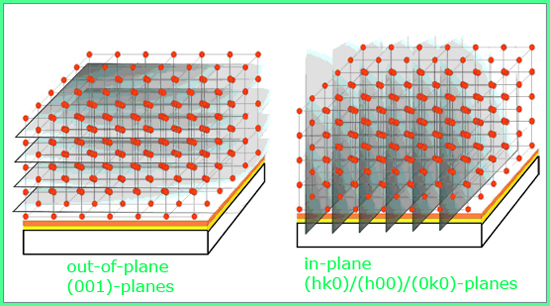
\includegraphics[width=0.8\textwidth]{lattice-planes-3d}
	\caption{Some lattice planes in the cubical lattice, now in 3D!}
	\label{fig:lattice-planes-3d}
\end{figure}

\newpage
These lattice planes plays an important role in the diffraction of incoming waves (usually light or more generally an electromagnetic wave). Thus it's important to identify different sets. This in done through \textbf{Miller indicies}. These indices are defined through where a plane intersects the crystal axes closest to it's origin, but not through the origin. By looking at figure~\ref{fig:lattice-planes-vis} we can see four different examples. If we let $\mathbf{a} = x$, $\mathbf{b}=y$ and $\mathbf{c} =z$ we can see how in (d) how we have a plane that intersects the crystal axes at $(\frac{\mathbf{a}}{1},\frac{\mathbf{b}}{1}, \frac{\mathbf{c}}{2})$. The Miller Indices is then the reciprocal of these factors we multiply the crystal axes with in order to find the intersect point, it's written as $(1 1 2)$. if a plane is parallel to a particular axis it's taken at a zero. 

\begin{figure}[H]
	\centering
	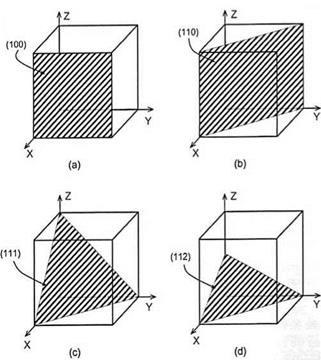
\includegraphics[width=0.8\textwidth]{lattice-planes-vis}
	\caption{Some lattice planes in the rectangular lattice, visually in 3d!}
	\label{fig:lattice-planes-vis}
\end{figure}

\newpage
We should also note that from an atomic view a certain amount of planes could due to symmetry in the crystal lattice be equivalent to eachother. This is depicted in figure~\ref{fig:lattice-planes-symmetry}. All these three planes are said to belong to the \textbf{form} $\{100\}$.
\begin{figure}[H]
	\centering
	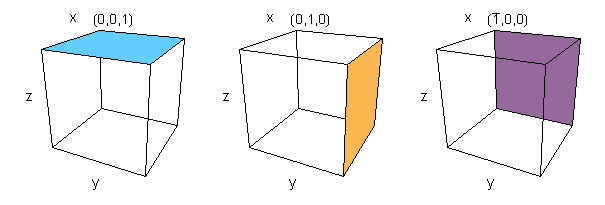
\includegraphics[width=0.8\textwidth]{lattice-planes-symmetry}
	\caption{These lattice planes is equivalent from an atomic point of view, thus all these three are written as belonging to the form $\{100\}$}
	\label{fig:lattice-planes-symmetry}
\end{figure}

One often want to specify the directions of a vector $\mathbf{r}$ in a crystal. A vector can be written as 
\begin{equation}
	\mathbf{r} = u\mathbf{a} + v \mathbf{b} + w \mathbf{c}
\end{equation}
We then refer to it as the $[uvw]$ direction. Due to symmetry in cubic crystals the $[uvw]$ direction is actually the normal to the $(uvw)$ plane. It should however be noted that this an exception and only hold for lattices with the particular symmetries of the cubic lattice.

\newpage
\subsection{Typical crystal structures}
Imagine that the atoms act like spheres, so if we wanna tightly pack them it's like packing cannon balls\footnote{This is actually very close to the truth since the atoms interact with each other with a force that is radial.}. This is depicted in figure~\ref{fig:packed-spheres}. The layer depicted can be stacked upon with another layer with spheres in the A,B or C positions. Now packing the other layer on the A position is neither stable nor efficient, and something that generally don't happen in nature. But depending on how the stacking structure looks like in an atom the solid gets a different structure which can be described by different lattices. 
\begin{figure}[H]
	\centering
	\includegraphics[width=0.8\textwidth]{packed-spheres}
	\caption{packed spheres! in 2d!}
	\label{fig:packed-spheres}
\end{figure}
\subsubsection{Cubic and hexagonal close-packed structures}
The ABCABC\ldots stacking yields the \textbf{face-centred cubic} structure, its conventional non-primitive unit cell is depicted in figure~\ref{fig:fcc}.
\begin{figure}[H]
	\centering
	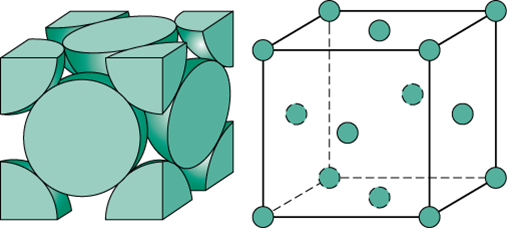
\includegraphics[width=0.8\textwidth]{fcc}
	\caption{The face centred cubic}
	\label{fig:fcc}
\end{figure}
\subsubsection{The body-centred cubic structure}
The body centred cubic structure is not quite close packed, so has no real equivalent to the packing sequence as the fcc does. This is due to certain positions are missing in this structure. In reality we can defend this lack of atoms due to the repelling forces among the atoms. The structures conventional non-primitive cell is depicted in figure~\ref{fig:bcc}.
\begin{figure}[H]
	\centering
	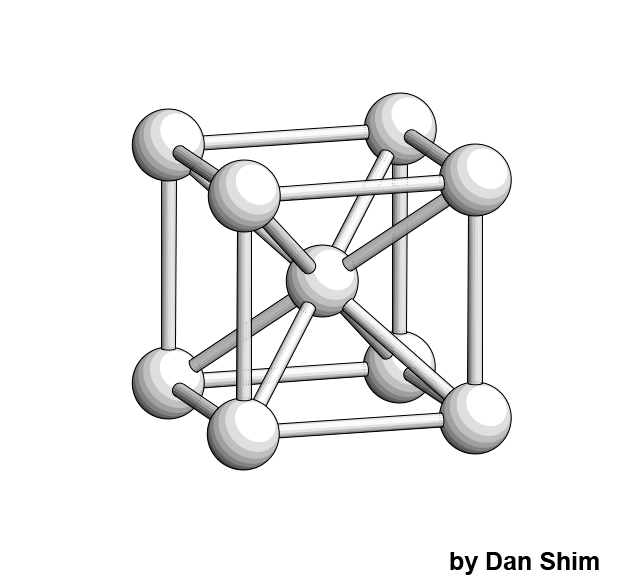
\includegraphics[width=0.8\textwidth]{bcc}
	\caption{The body centred cubics non-primitive conventional cell}
	\label{fig:bcc}
\end{figure}

\newpage
\subsubsection{Structures of ionic solids}
Ionic soldis are simply a crystal containing more then one element(or a specific type of an atom as we will more specifically look at). In figure~\ref{fig:nacl} we can see atomic structure of the NaCl molecule.  EElectrons in the negatively charged anion(Cl) are generally less tightly bund than those in the positively charge anion(Na). By convention we write the lously bounded anion as the bigger atom in our structure. 

It's interesting to note that we have $(111)$ planes in this lattice as showed here which will create planes of only Na or Cl atoms. That can be showed through it's diffraction properties. 
\begin{figure}[H]
	\centering
	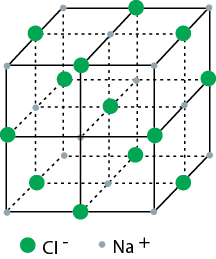
\includegraphics[width=0.8\textwidth]{nacl}
	\caption{The ionic structure of the NaCl solid}
	\label{fig:nacl}
\end{figure}
\newpage
\subsubsection{The diamond and zincblende structures}
A more advanced structure which basically can be constructed through a cubic lattice and a more complex basis. This structure is showed in figure~\ref{fig:zincblende-structure}. It's interesting that the structure is identitical for zincblende and diamonds, the only difference is that diamonds are only carbon, while zincblende is made from zinc and  sulfur.
\begin{figure}[H]
	\centering
	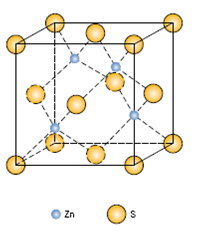
\includegraphics[width=0.8\textwidth]{zincblende-structure}
	\caption{The structure for zincblende. Note that it's the same for diamonds except for diamonds you only have carbon}
	\label{fig:zincblende-structure}
\end{figure}

\newpage
\subsubsection{The Wigner-Seitz cell}
By taking the planes that goes perpendicularly  through all the bisects of the lines to an atoms neighbours, one end up with its Wigner-Seitz cell. This represents the "sphere of influence". For the fcc such a cell has twelve neighbours and twelve faces, thus all the sites in fcc has a \textbf{coordination number} of twelve.

Always a primitive cell.
\begin{figure}[H]
	\centering
	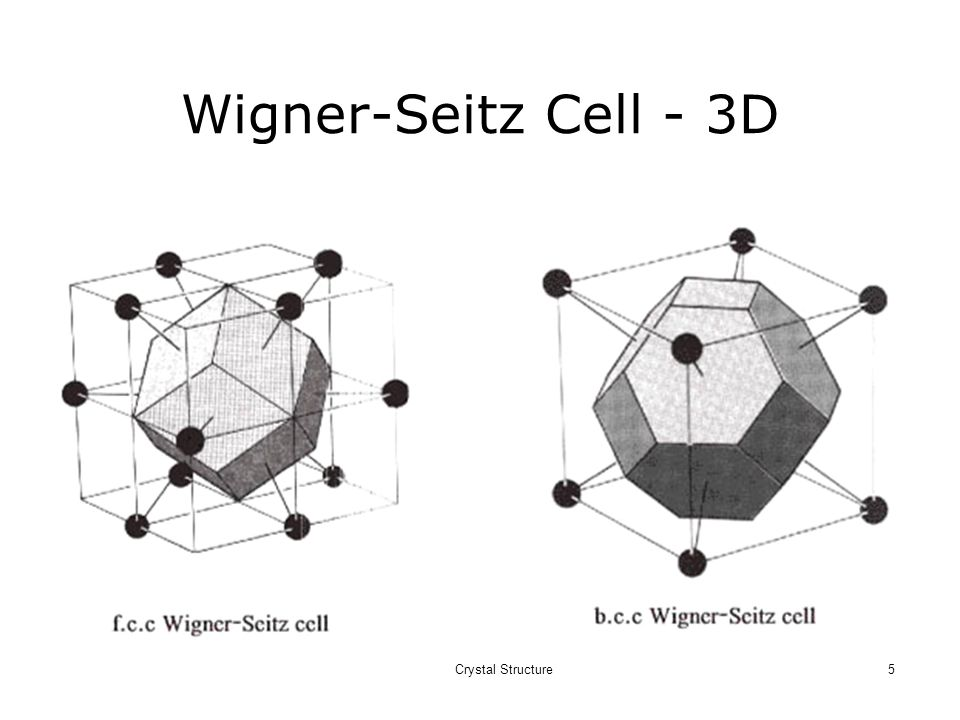
\includegraphics[width=0.8\textwidth]{wigner-seitz}
	\caption{The Wigner-Seitz cell for the fcc and bcc structure}
	\label{fig:wigner-seitz}
\end{figure}

\newpage
\subsection{X-ray crystallography}
\subsubsection{The Bragg  law}
Bragg law is a simplified way of looking at the reflection from crystal structures. Instead of using the general laws of diffraction as von Laue did, we will just see lattice planes as "reflective planes". One can then use Braggs law to help identify crystal structures
\begin{equation}
	2d\sin{\theta} = n\lambda
\end{equation}
We can have reflections of higher orders ($n>1$). If we for instance get a reflection of the third order from the plane $(111)$ we call it through convention the reflection of plane $(333)$. In general terms a nth order reflection of a plane $(hkl)$ is written as a reflection from plane (nh nk nl).

\begin{figure}[H]
	\centering
	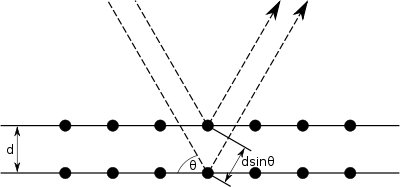
\includegraphics[width=0.8\textwidth]{bragg}
	\caption{The reflection due to lattice planes}
	\label{fig:bragg-law}
\end{figure}

\subsubsection{Experimental arrangements for x-ray dirffraction}
\newpage
\paragraph{A Laue photograph} is depicted in figure~\ref{fig:laue-photograph}. It is usually a good at showing symmetries, thus a good tool for figuring out the orientation of a crystal.
\begin{figure}[!ht]
	\centering
	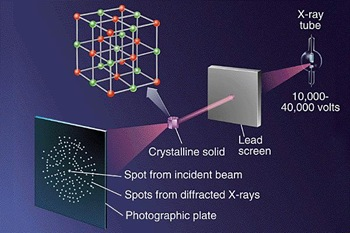
\includegraphics[width=0.8\textwidth]{laue-photograph}
	\caption{The experimental setup for the Laue photograph}
	\label{fig:laue-photograph}
\end{figure}

\newpage
\paragraph{A Rotating crystal and powder photograph} is depicted in figure~\ref{fig:rotating-crystal}. It's a tool better suited for analysing the actual structure of a crystal.
\begin{figure}[!ht]
	\centering
	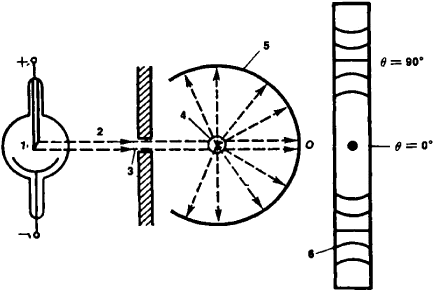
\includegraphics[width=0.8\textwidth]{rotating-crystal}
	\caption{The basic setup for a rotating crystal photograph or powder photograph. The difference is wether on not the speciment in the middle is a rotating crystal or a powder of crystalline crystals.}
	\label{fig:rotating-crystal}
\end{figure}

\newpage
\subsection{Interatomic forces}
\subsubsection{Van der Waals bonding}
Van der Waals occurs with even stable atoms, those who has all the outer electrons in their shell. This is due to flutuation that creates an electric dipole moment. This force experienced is described by the Lennard-Jones potential depicted in figure~\ref{fig:lennard-jones}. Worth noting that the repulsive force is a consequence of the Pauli principle, that states that no two electrons can occupy the same state, and instead the electrons get excited to higher state if another one would come close. This creates a large repulsive force which one clearly see in the Lennard-Jones potential.
\begin{figure}[!ht]
	\centering
	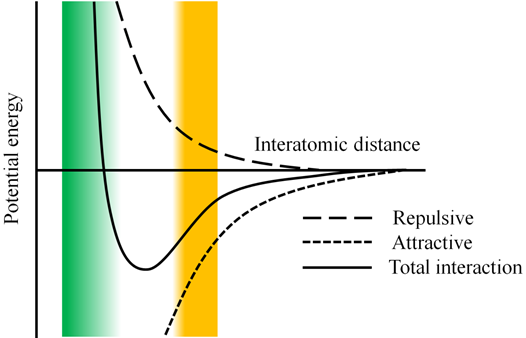
\includegraphics[width=0.8\textwidth]{lennard-jones}
	\caption{The Lennard-Jones potential is the main force in Van der Waals bonding. The color green represent a distance in which repulsion occurs, while the color of orange represents a distance of attraction. Kinda like how it is with us humans too lol.}
	\label{fig:lennard-jones}
\end{figure}

\newpage
\subsubsection{Ionic bonding}
Basically ionic bonding is the process of atoms sharing one electron in order to create two charged atoms with completed outer shells. The truth goes of course down too Schrödinger's, but in this is as far as we go to it now.
\begin{figure}[!ht]
	\centering
	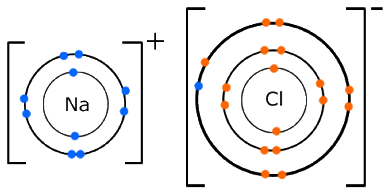
\includegraphics[width=0.8\textwidth]{ionic-bond}
	\caption{The ionic bond between Na and Cl. In this example Na gives away its stray atom in its outer shell in order to complete the outer shell of Cl. The reality is more complex, but deeply related to electron states in the shells.}
	\label{fig:ionic-bond}
\end{figure}

\newpage
\subsubsection{Covalent bonding}
The covalent bonding is similar to the ionic bonding in the sharing of electrons. The covalent bond has some more complexity related to it. It's usually directed too, so can, among other things, be a factor of why there exists solids which has more complex structures. Basically atoms can share electrons between multiple atoms in order for all the outer shells to saturated. This is depicted in figure~\ref{fig:covalent} for the famous $H_2O$ molecule.

\begin{figure}[!ht]
	\centering
	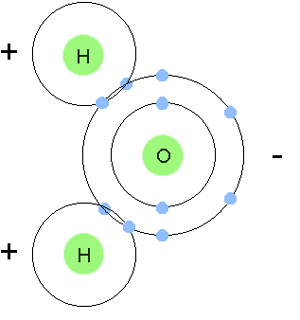
\includegraphics[width=0.8\textwidth]{covalent}
	\caption{The covalent bond is similar to the ionic bond, but shares multiple electrons, could be over multiple atoms and those usually have some kind of direction related to it.}
	\label{fig:covalent}
\end{figure}

\subsubsection{Hydrogen bonding}
Looking at the earlier picture of the $H_2O$ molecule in figure~\ref{fig:covalent}, we can see that the molecule itself has a negative and positive charge. This causes important bindings in ice and many organic solids.

\newpage
\subsubsection{Metallic bonding}
In the metallic bond we have a kind of covalent bond which does not saturate the outer shell of the atoms. This results in "wandering atoms" as depicted in figure~\ref{fig:metallic-bonding}. This in turns facilitate the ability to conduct electricity. 
\begin{figure}[!ht]
	\centering
	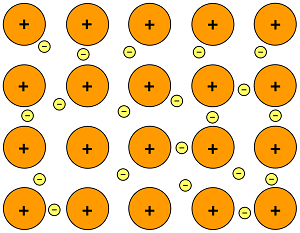
\includegraphics[width=0.8\textwidth]{metallic-bonding}
	\caption{In the metallic bond the atoms share their electrons more freely}
	\label{fig:metallic-bonding}
\end{figure}

\newpage
\subsubsection{Mixed bonding}
Basically just highlighting that we can more then one bond in a solid. As an example we have graphite as depicted in figure~\ref{fig:graphite-bond}. There we have both a covalent bond in the layer, as well a Van der Waals bond between layers. This causes graphite to have the interesting effect of only conducting electricity in the direction parallel to the layers, not perpendicular to it (and thus the Van der Waals bond does not conduct electricity especially well).
\begin{figure}[!ht]
	\centering
	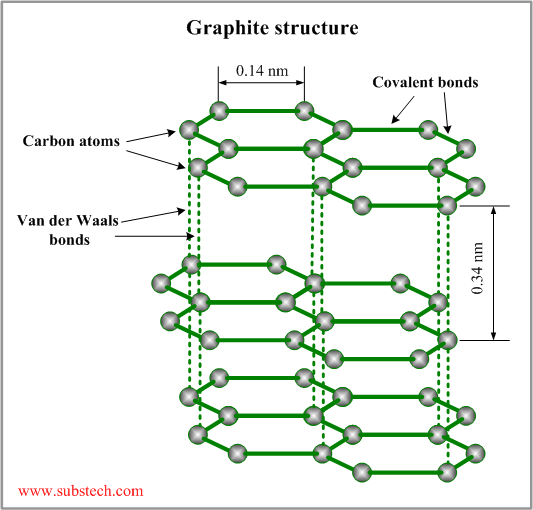
\includegraphics[width=0.8\textwidth]{graphite-bond}
	\caption{Depicting the mixed bond inside graphite. Each layer has strong covalent bond, while between layers only Van der Waals forces keeps it together.}
	\label{fig:graphite-bond}
\end{figure}
\newpage 
\subsection{New Words}

\begin{itemize}
	\item \textbf{crystal lattice}
	\item \textbf{translational invariance}
	\item \textbf{unit cell}
	\item \textbf{rectangular lattice}
	\item \textbf{rhombic lattice}
	\item \textbf{centred rectangular lattice}
	\item \textbf{point symmetry groups}
	\item \textbf{crystal classes} 
	\item \textbf{space symmetry groups}
	\item \textbf{Miller indicies}
	\item \textbf{face-centred cubic}
	\item \textbf{coordination number}
\end{itemize}

\newpage
\section{Waves in crystals}

\subsection{Elastic scattering of waves by a crystal}
\subsubsection{Amplitude of the scattered wave}
Using braggs law we were able to find where we should have reflections. But we know nothing of the amplitude. This we will find out by examining every atom as a point source for radial radiation. This radial radiation gets created when excited, or radiation has hit it. The setup for this thought process is depicted in figure~\ref{fig:crystal-plane-wave}. 

Lets assume the incident radiation is a plane wave on the form $A_0 \exp{[i(\mathbf(k) \cdot \mathbf{r} - \omega t)]}$. The resulting amplitude of the radiation at the detector is then
\begin{equation}
	A_r = A_0 e^{i(\mathbf{k} \cdot \mathbf{r} - \omega t)} \times f \times \frac{e^{ik(|\mathbf{R} - \mathbf{r}|)}}{|\mathbf{R}-\mathbf{r}|}.
\end{equation}

\begin{figure}[!ht]
	\centering
	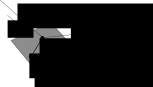
\includegraphics[width=0.8\textwidth]{crystal-plane-wave}
	\caption{An incoming plane wave towards a crystal and description of what part radial excitation wave will hit the detector}
	\label{fig:crystal-plane-wave}
\end{figure}

We can see three terms in the right hand side of this equation. We will number them as they appear in the equation. The first part is just the incoming wave. The second part is the \textbf{atomic form factor} or \textbf{atomic scattering factor}, which defines how much radiation a certain atom will scatter. The third term is the apmlitude decrese and phase change due to the position of an atom. Assuming that the distance of the detector from the crystal is insanely much larger then the crystal atom distances we can simplify the third term to be
\begin{equation}
	\frac{e^{ik(|\mathbf{R} - \mathbf{r}|)}}{R}.
\end{equation}
We go on to define the \textbf{scattering vector} $\mathbf{K}$ as 
\begin{equation}
	\mathbf{K} = \mathbf{k}'-\mathbf{k}
\end{equation}
We can also apparently sag that $k \cdot |\mathbf{R}-\mathbf{r}| \approx \mathbf{k}'\cdot (\mathbf{R}-\mathbf{r})$. So we end up with a term for the amplitude as 
\begin{equation}
	A_r \approx A_0 \frac{e^{i(k\mathbf{R}-\omega t)}}{R} f e^{-i\mathbf{K} \cdot \mathbf{r}}
\end{equation}
The first term in this equation is the same for all atoms in a structure, so it can be factored out as a constant. We are left with knowing that the amplitude is proportional to
\begin{equation}
	A = \sum_n f_n e^{i\mathbf{K} \cdot \mathbf{r}_n}
\end{equation}
where the sum is over all atoms in the crystal.

Recalling that the position of an atom can be made up of lattice point position and its basis inside that we can split $\mathbf{r}$ into its lattice association $\mathbf{r}_l$ and position relative to the lattice point(using the basis) $\mathbf{r}_p$. This idea is depicted in figure~\ref{fig:basis-sep}. The equation then becomes
\begin{equation}
	A = \sum_l  e^{i\mathbf{K} \cdot \mathbf{r}_l} \times \sum_p f_p e^{i\mathbf{K} \cdot \mathbf{r}_p}
	\label{eq:ampl}
\end{equation}
The first part of this right hand expression is what determines the direction for which diffraction occurs and is due to the crystal lattice. The second part is due to the basis, and is the same for all lattice points, which is a sum over relatively few atoms. This second part is called the \textbf{structure factor}.

\begin{figure}[!ht]
	\centering
	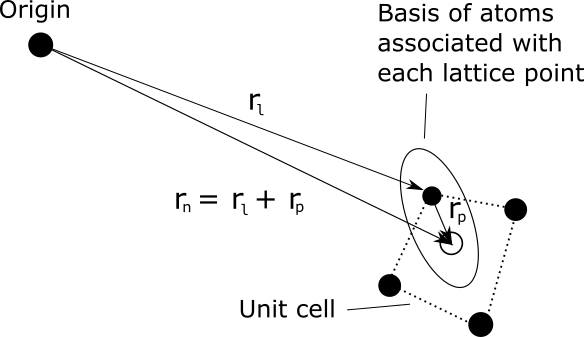
\includegraphics[width=0.8\textwidth]{basis-sep}
	\caption{}
	\label{fig:basis-sep}
\end{figure}

\newpage
\subsubsection{Laue conditions for diffraction and the reciprocal lattice}
Using equation~\ref{eq:crystal-lattice-3d} for the crystal lattice, and the first term in equation~\ref{eq:ampl} we get
\begin{equation}
	\sum_l e^{i\mathbf{K} \cdot \mathbf{r}_l} =\sum_u e^{i\mathbf{K} \cdot \mathbf{a}u} + \sum_v e^{i\mathbf{K} \cdot \mathbf{b}_v} + \sum_w e^{i\mathbf{K} \cdot \mathbf{c}w}.
\end{equation}
Since we only get a large scattering amplitude when the contribution from all the lattice point are in phase, we get the requirement that
\begin{align}
	\mathbf{K} \cdot \mathbf{a} &= 2\pi h \\
	\mathbf{K} \cdot \mathbf{b} &= 2\pi k \\
	\mathbf{K} \cdot \mathbf{c} &= 2\pi l 
\end{align}
where $h,k,l$ is integers. This is what we call the \textbf{Laue conditions} for diffraction. When these requirements are satisfied we get unity from the lattice term in amplitude for every lattice point and we end up with the number of primitive unit cells as the lattice term.

The directions of the diffracted beams are thus given by the set of vectors $\mathbf{k}$ that satisfies the Laue conditions. It turns out that this set of vectors are actually the reciprocal of the lattice vectors! I.e.
\begin{equation}
	\mathbf{K} = h\mathbf{a^*} + k\mathbf{b^*} + l \mathbf{c^*}
\end{equation}
where 
\begin{align}
	\mathbf{a^*} &= \frac{2\pi(\mathbf{b}\times\mathbf{c})}{\mathbf{a}\cdot(\mathbf{b}\times\mathbf{c})} \nonumber\\
	\mathbf{b^*} &= \frac{2\pi(\mathbf{c}\times\mathbf{a})}{\mathbf{a}\cdot(\mathbf{b}\times\mathbf{c})} \nonumber\\
	\mathbf{c^*} &= \frac{2\pi(\mathbf{a}\times\mathbf{b})}{\mathbf{a}\cdot(\mathbf{b}\times\mathbf{c})} 
	\label{eq:reciprocal-lattice}
\end{align}
The book proves in page 321 that braggs and this requirements both holds up.

Since the scattering vector of each diffracted beam corresponds to a point in reciprocal lattice, we can use the integers $h,k,l$ to label the beams. These labels are identical to the miller indices of the lattice plane that is associated with the diffracted beam, this is also proved in the book at page 321.   

To surmise: for an incident radiation of wavevector $\mathbf{k}$, the direction of the diffracted beams are given by wave vectors $\mathbf{k'} = \mathbf{k} + \mathbf{K}$, where the scattering vector $\mathbf{K}$ is any one of the points of the reciprocal lattice for the crystal. You determine the $\mathbf{K}$ vector through equations~\ref{eq:reciprocal-lattice}.

\subsubsection{Examples of reciprocal lattices}
In describing these reciprocal we will use the three mutually perpendicular real value unit vectors $mathbf{i}$, $mathbf{j}$, $mathbf{k}$.
\paragraph{The simple cubic real space lattice} is going to be investigated first!
In terms of Cartesian axes we have 
\begin{align}
	\mathbf{a} &= a\mathbf{i} \nonumber\\
	\mathbf{b} &= a\mathbf{j} \nonumber\\
	\mathbf{c} &= a\mathbf{k} 
\end{align}
using equation~\ref{eq:reciprocal-lattice} we get the reciprocal

\begin{align}
	\mathbf{a} &= \frac{2\pi}{a}\mathbf{i} \nonumber\\
	\mathbf{b} &= \frac{2\pi}{a}\mathbf{j} \nonumber\\
	\mathbf{c} &= \frac{2\pi}{a}\mathbf{k}  
\end{align}
Basically just the same with shorter sides!

\newpage
\paragraph{The face-centred cubic real space lattice} is intriguingly connected with the bcc. We start with define the fcc as
\begin{align}
	\mathbf{a} &= \frac{a}{2} (\mathbf{j} + \mathbf{k}) \nonumber\\
	\mathbf{b} &= \frac{a}{2} (\mathbf{k} + \mathbf{i}) \nonumber\\
	\mathbf{c} &= \frac{a}{2} (\mathbf{i} + \mathbf{j}) 
\end{align}
which gives us the reciprocal
\begin{align}
	\mathbf{a} &= \frac{2\pi}{a} (\mathbf{j} + \mathbf{k} - \mathbf{i}) \nonumber\\
	\mathbf{b} &= \frac{2\pi}{a} (\mathbf{k} + \mathbf{i} - \mathbf{j}) \nonumber\\
	\mathbf{c} &= \frac{2\pi}{a} (\mathbf{i} + \mathbf{j} - \mathbf{k}) \nonumber\\
\end{align}
Which yields the bcc! Not completely visible perhaps, maybe easier to see through the reciprocal equations directly perhaps. But basically the vectors get translated around to the bbc, and scaled of course, this is depicted in figure~\ref{fig:fcc-bcc}.
\begin{figure}[!ht]
	\centering
	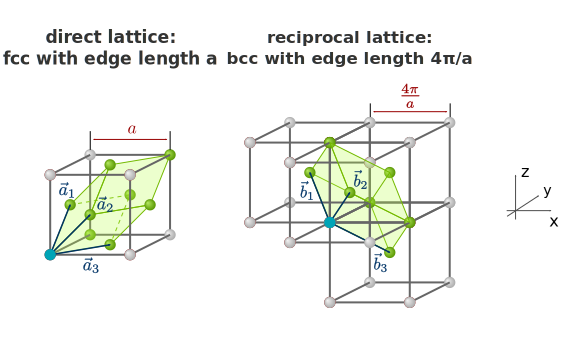
\includegraphics[width=0.8\textwidth]{reciprocal-lattice-fcc-bcc}
	\caption{Here we can see how the reciprocal of the fcc lattice is just rotated and scaled into a bcc lattice}
	\label{fig:fcc-bcc}
\end{figure}

\newpage
\subsubsection{The structure factor}
Now it's time we look at the second part of equation~\ref{eq:ampl}. This part 
\begin{equation}
	S = \sum_p f_p e^{-i\mathbf{K} \cdot \mathbf{r}_p}
	\label{eq:structure-factor}
\end{equation}
is known as the structure factor and only concerns the basis in the structure. 

\paragraph{The simplest form} of structure factor occurs when we only have one atom at each lattice point. This then reduces to be 
\begin{equation}
	S = f
\end{equation}
where f is only dependent on the incident angle and what kind of atoms that occurs on the lattice.

\newpage
\paragraph{Using the hexagonal close packed structure}, as depicted in figure~\ref{fig:hcp}, we get another basis 
\begin{align}
	\mathbf{r}_1 &= \mathbf{0} \\
	\mathbf{r}_2 &= \mathbf{a}/3+\mathbf{b}(2/3) + \mathbf{c}/2
\end{align}
So if we put this into the structure factor equation~\ref{eq:structure-factor} and use the reciprocal equation~\ref{eq:reciprocal-lattice}, we get
\begin{equation}
	S = f\{1+\exp{[-i\pi((h+k+l)+(k-h)/3)]}\}
\end{equation}
Since the amplitude is proportional to $S$, we can use this equation to do some analysis of where the amplitude might completely go to zero. But also to some extend see which planes will have a large contribution to reflections. This of course have to weighted against the lattice term as well.

We also have to note we haven't looked into the atomic factor at all. It could differ for the same atoms as well due to different environment and such. This have an effect on structures like the diamond.
\begin{figure}[!ht]
	\centering
	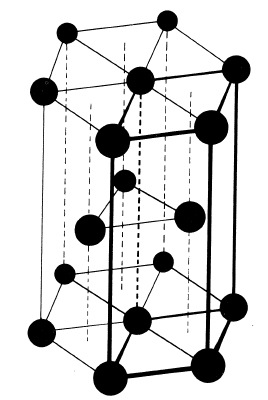
\includegraphics[width=0.4\textwidth]{hcp}
	\caption{The hexagonal close packed structure.}
	\label{fig:hcp}
\end{figure}

\newpage
\section{Diamagnetic and paramagnetism}
\subsection{Introduction}
The increase in a magnetic field applied to any material(referred to as $\mathbf{H}$) causes an induced electromotive force, which in turn accelerates electrons in the material. Then according to Lenz's law the resulting electric current is such that it reduces the magnetic field applied inside the material, one also say that the magnetic field is ``screened'' from the material.

What's more interesting is that this current actually still exist even if the magnetic field is held at a constant value\footnote{We will explain this phenomenon later.}. If this does indeed happen in a material, then the material is \emph{diamagetic}. Note that the current creates a magnetic field, Denoted as $\mathbf{M}$, which works against the applied magnetic field, $\mathbf{H}$.

If a material posses atoms with a permanent magnetic dipole moment\footnote{Think bar magnets.}, then the diamagnetic effects are usually very small in comparison to the \emph{paramagnetic} effects. The paramagnetic effect creates a magnetization, $\mathbf{M}$, which works with the applied magnetic field, $\mathbf{H}$. 

We can relate the magnetization of the material, $\mathbf{M}$, with the applied magnetic field, $\mathbf{H}$ through the \emph{magnetic susceptibility}, $\chi$, of the material as 
\begin{equation}
	\mathbf{M} = \chi \mathbf{H}.
	\label{eq:susceptibility}
\end{equation}
From this we can deduce the sign of the magnetic susceptibility will be positive for paramagnetic materials and negative for diamagnetic materials. 

\subsection{Paramagnetism}
\subsubsection{The origin of permanent dipole moments}
From ampere's law we can deduce an equation for the magnetic dipole moment, $\pmb{\mu}$, to be
\begin{equation}
	\pmb{\mu} = i \pmb{a}.
	\label{eq:amperes-law}
\end{equation}
Where $\pmb{a}$ is the area vector of the loop, directed so that the current is clockwise when looking along $\pmb{a}$. and $i$ is the electric current.

To start with we can look at the dipole moment of a electron going around it's nucleus with a period of $\tau$, and a radius $r$. The current is then 
\begin{equation}
	i = (-e)/\tau = -e v/2\pi r.
\end{equation}
Where the negative sign comes from the fact that the electron moves in the opposite direction of the current\footnote{Thank you convention for making everything confusing!}. Rewriting the dipole moment with this current we get
\begin{equation}
	\pmb{\mu} = - \frac{ev}{2\pi r} \pmb{a}.
\end{equation}
Now we can use the angular moment of the electron which is $\hslash \pmb{I}$. The $\hslash$ is just convention, as we know constants can be multiplied in and divided away as long as it's done in a balanced matter. If we see that $|\pmb{a}| = \pi r^2$, $|\hslash| = mvr$ and that $\pmb{a}$ and $\pmb{I}$ is directed in the same direction, we can rewrite the dipole moment as
\begin{equation}
	\pmb{\mu} = - \frac{e\hslash}{2m} \pmb{I}.
	\label{eq:orbital_momentum}
\end{equation}
We can then define the constant part as the Bohr magneton, $\mu_B$, i.e.
\begin{equation}
	\mu_B = \frac{e\hslash}{2m} = 9.27 \times 10^{-24} J T^{-1}.
\end{equation}

Now we've used the classical model of an electron spinning around its nucleus to figure out the dipole moment contribution due to the orbital angular momentum of the electron through equation~\ref{eq:orbital_momentum}. But due to hand waviness, we're gonna go the quantum mechanical route with this equation. Thus we have an equation 
\begin{equation}
	\pmb{\mu} = -\mu_B \pmb{I}
\end{equation}
for the orbital angular momentum, but also a magnetic dipole moment is given for the spin in the quantum mechanical treatment that is as follows
\begin{equation}
	\pmb{\mu_{spin}} = - g_0 \mu_B \pmb{S}.
\end{equation}
And we estimate $g_0=2$\footnote{Sorry, too intricate to explain} and we get a total magnetic dipole moment to be
\begin{equation}
	\pmb{\mu} = - \mu_B (\pmb{L}+2\pmb{S}).
	\label{eq:total_angular_momentum}
\end{equation}
Where $\pmb{L}$ is the total sum of atoms electron orbital momentums and $\pmb{S}$ is the sum of the atoms electrons spin angular momenta. For every closed shell this sum adds up to be zero. Thus permanent dipole moments only occur in atoms or ions with an incomplete shell. 

To look at how an incomplete shell is built for incomplete shells in isolated ions, and thus being able to calculate the momenta of them, we use the Russell-Sounders coupling scheme, or L-S coupling. It states that the stationary states of the shell are eigenstates of $\pmb{L^2}, \pmb{S^2}$ and $\pmb{J^2}$, with eigenvalues $L(L+1), S(S+1)$ and $J(J+1)$. To find the values of L,S and J we use the Hund's rules
\begin{enumerate}
	\item S takes the maximum value allowed by the exclusion principle, thus as many as possible of the electrons have parallel spins
	\item L takes the maximum value consistent with this value of S - the electrons have their orbital angular momenta as well aligned as possible
	\item $J = |L-S|$ for shells less then half full and $J = L+S$ for shells more then half full.
\end{enumerate}

Here it's interesting to note that rule 1 and 2 of Hund's rules are closely associated with the Coulomb forces between electrons, due to them being much larger then the magnetic force\footnote{Not argued for here, but take my word for it!}. And the value of j, is associated with the spin-orbit interaction, that is with the magnetic field generated by the motion of the electrons within the atom, this is of order 10T\footnote{Also just a given fact}. So the 3rd rule can be effected by a field applied of this order.

In figure~\ref{fig:hunds} we get a picture of two ions having applied the Hund's rule on to determine the values of L,S and J. 

\begin{figure}[!ht]
	\centering
	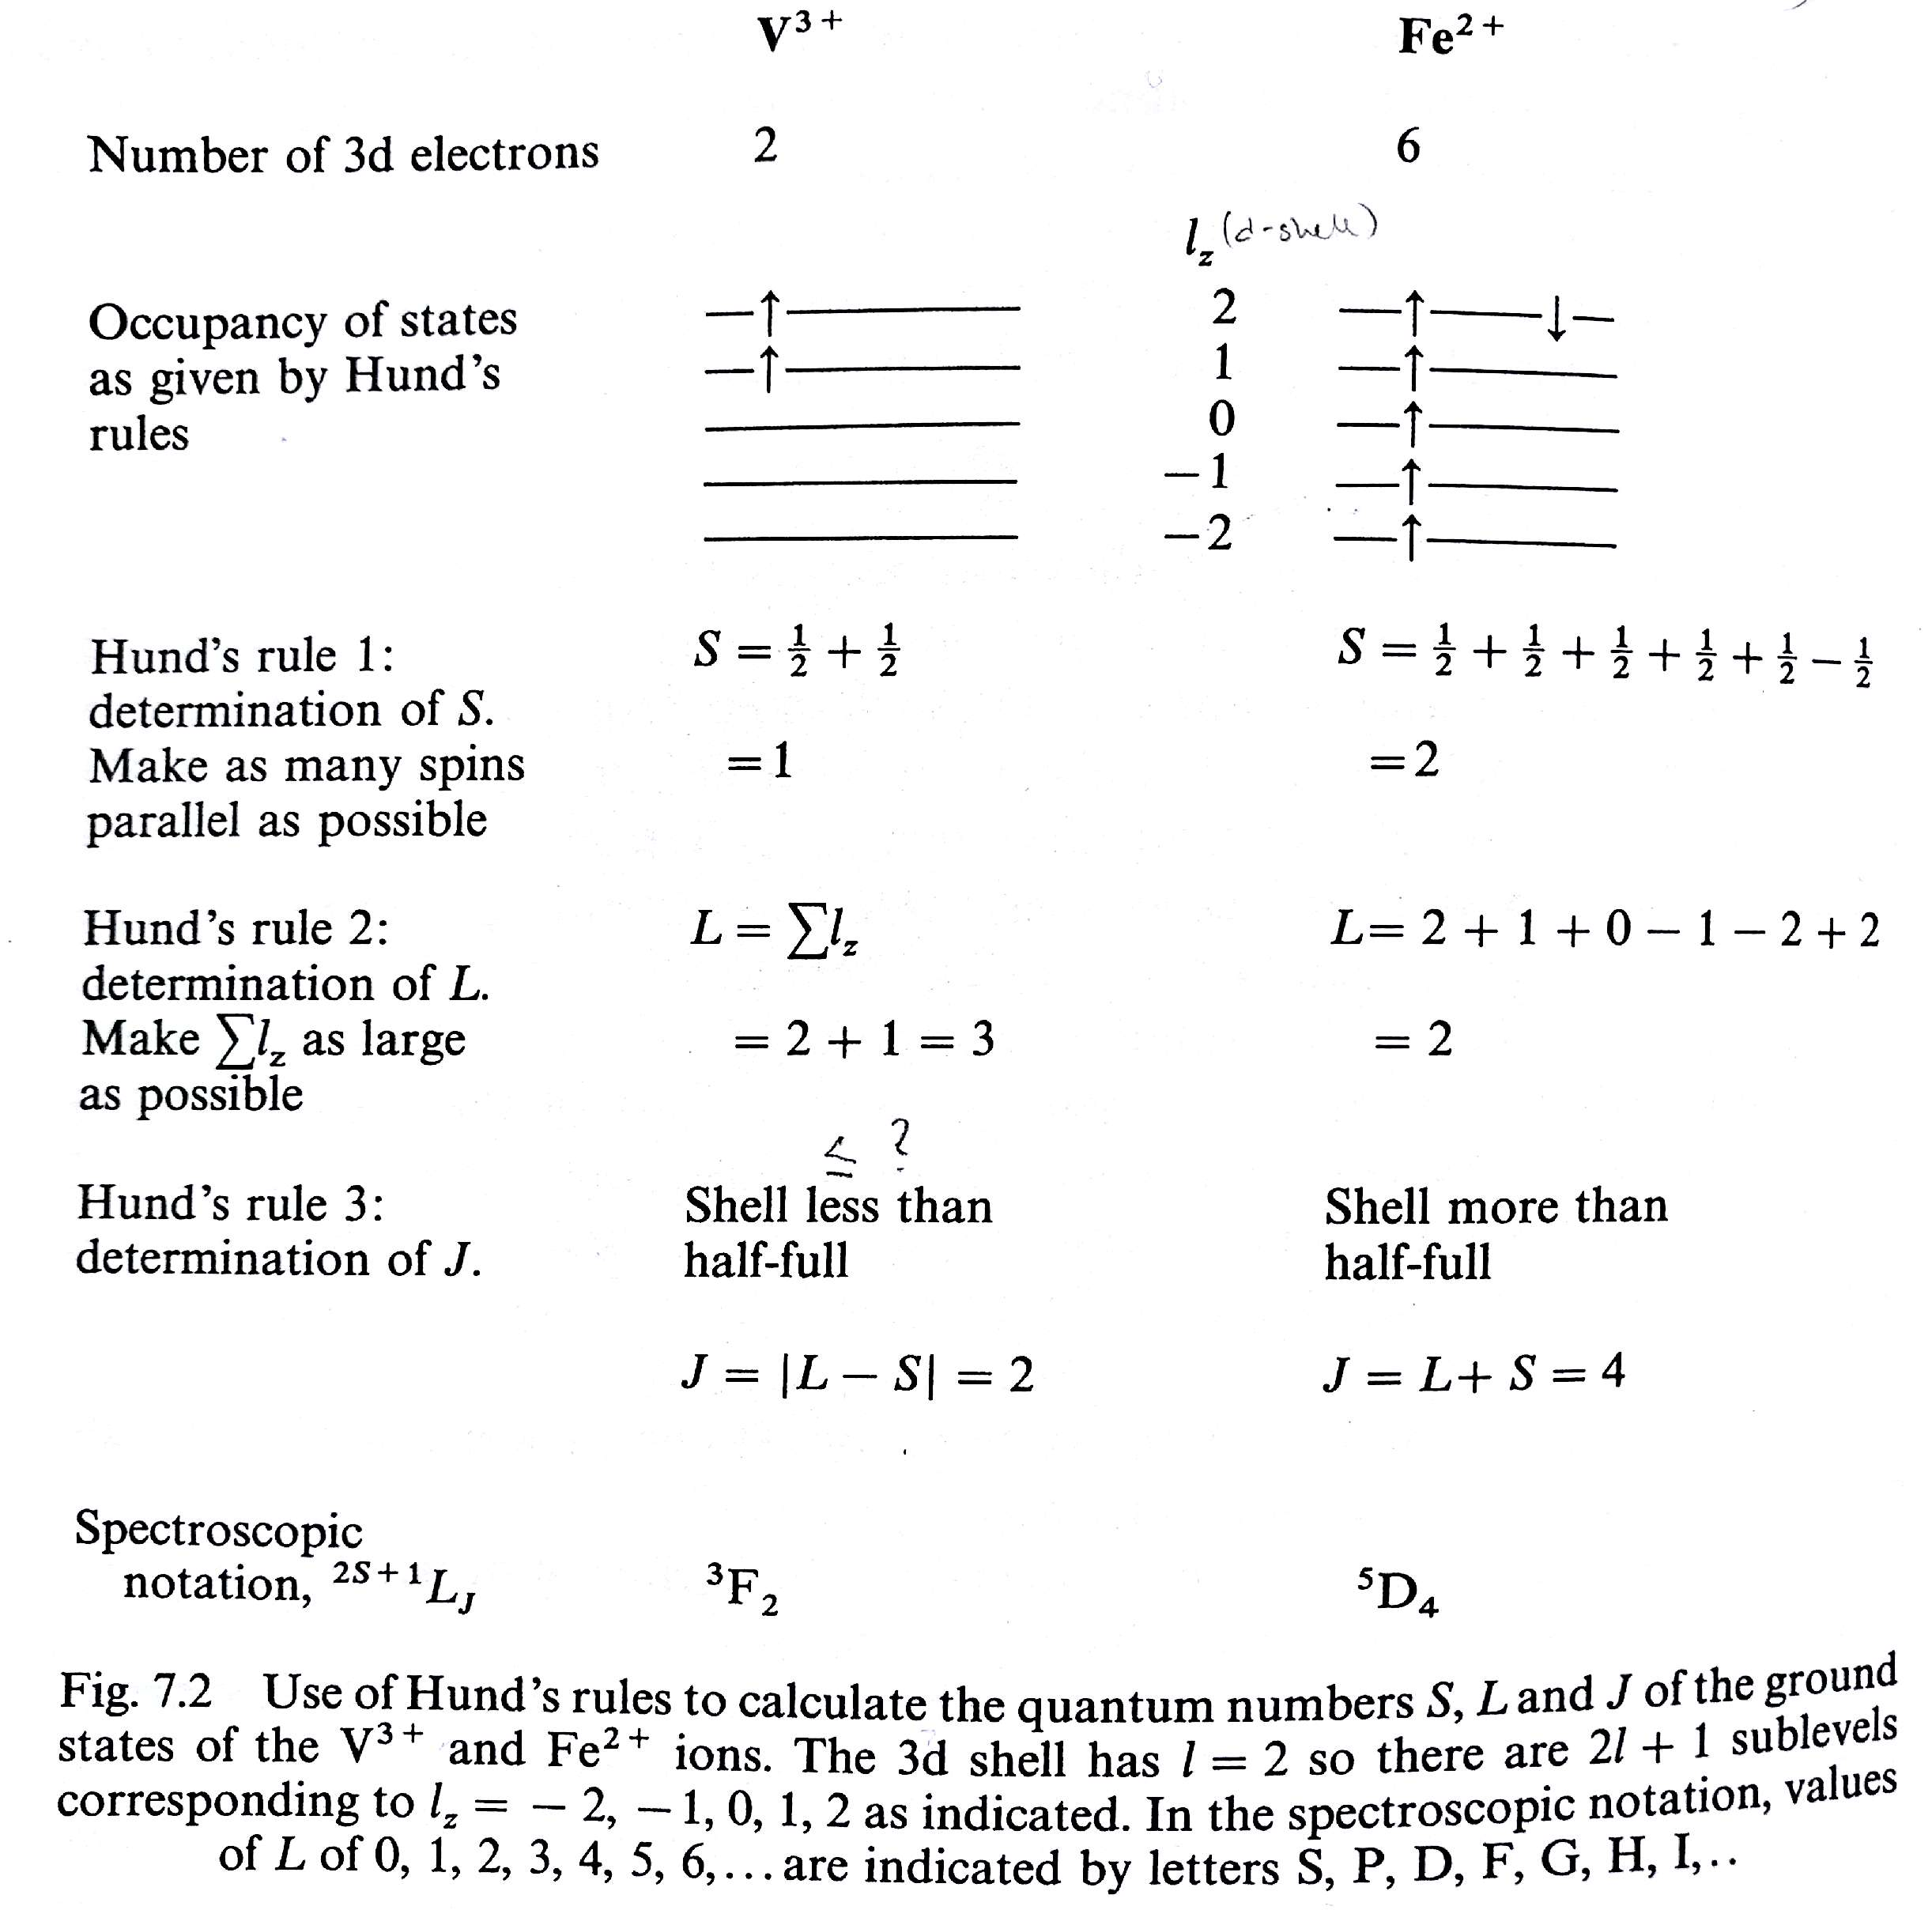
\includegraphics[width=\textwidth]{hunds}
	\caption{Copied from Solid State Physics by J.R. Hook and H.E. Hall}
	\label{fig:hunds}
\end{figure}

\subsubsection{The interaction of permanent dipole moment with an applied magnetic field}
Alignment of an atomic dipole by a field $\pmb{B}$ (which is taken to be along the z-axis) occurs because of an energy term in the electrons, $H_P$,
\begin{equation}
	H_P = - \pmb{\mu} \cdot \pmb{B} = -\mu_z B.
	\label{eq:alignment_energy}
\end{equation}
Where $\pmb{\mu}$ is given by equation~\ref{eq:total_angular_momentum}. It should however be noted that you should not think of it as an atomic bar magnet, because things does not quite act the same on the atomic level as things does in the macroscopic world\footnote{But of course it does now just to be confusing.}. For instance this $H_p$ energy is actually part of the kinetic energy of the atom.

\newpage
If we assume that the energy $H_p$ is small, we can use first-order perturbation theory to calculate the effect of the alignment energy. We then assume a ground state(nothing excited to a new level) for the ion, or atom, and use quantum hand waviness to get the expectation energy
\begin{equation}
	E_p = \langle H_p \rangle = g\mu_B J_z B
	\label{eq:expected_alignment_energy}
\end{equation}
where $j_z = -j,\ldots ,1,0,1,\ldots j$ and g is the \emph{Landé g-factor} 
\begin{equation}
	g = \frac{3}{2} - \frac{L(L+1) - S(S+1)}{2J(J+1)}
\end{equation}

Comparing equation~\ref{eq:alignment_energy} and equation~\ref{eq:expected_alignment_energy}, we can see that we seem to have an effective magnetic moment 
\begin{equation}
	\pmb{\mu}_{eff} = g\mu_B\pmb{J}
	\label{eq:effective-magnetic-moment}
\end{equation}
\subsubsection{Calculation of the magnetization of paramagnetic ions}
Now, finally, we have the energy which is due to the magnetic dipole moment in the electrons, maybe we could calculate the magnetization from the paramagnetic material given a certain temperature T and magnetic field $\pmb{B}$.

Well, if we look at every dipole as they where independent on each other, we can use the Boltzmann factor to figure out how the relative occupation of energy levels will be at a certain temperature T. The Boltzmann factor is given by
\begin{equation}
	e^{-E_p/k_B T} = e^{\pmb{\mu}_{eff} \cdot \pmb{B} / k_B T}
\end{equation}
and we did use equation~\ref{eq:expected_alignment_energy} here in order to complete our expression for the Boltzmann factor. We can go one step further and specify that the magnetization field is parallel to the z-axis and the expression becomes
\begin{equation}
	e^{\mu_{eff}^z B/k_B T}
\end{equation}
where 
\begin{equation}
	\mu_{eff}^z = -g\mu_B J_z.
\end{equation}
We can then write the net magnetization for N moments per unit volume, through our deep understanding of statistical physics, to be
\begin{equation}
	M = N \sum^{+J}_{J_z = -J} (e^{\mu_{eff}^z B/k_B T} / \sum^{+J}_{J_z = -J} e^{\mu_{eff}^z B/k_B T})
\end{equation}
Note that the J is baked into the $\mu_{eff}^z$ constant.

\newpage
Using some fancy rewrites and awesome algebraic skills we can get to another expression that is easier to study, which is
\begin{equation}
	M = Ng\mu_B J B_J(x)
	\label{eq:paramagnetic-magnetization}
\end{equation}
Where 
\begin{equation}
	x = g \mu_B BJ/k_B T
\end{equation}
and 
\begin{equation}
	B_J(x) = \frac{2J+1}{2J} \coth{[(\frac{2J+1}{2J})x]} - \frac{1}{2J}\coth{(\frac{x}{2J})}.
\end{equation}
Where $B_J(x)$ is known as the Brillouin function. This function has the interesting property of increasing linearly for small $x$, but saturates at $1$ for large $x$. Thus for small fields applied to a paramagnetic material the resulting magnetization in the material increases linearly to then reach the \emph{saturation magnetization} $Ng\mu_B J$ when a large field is applied. 

For small fields(or rather small $x$) we can approximate $B_J(x)$ to be
\begin{equation}
	B_J(x) \approx \frac{(J+1)x}{3J}.
\end{equation}
So the resulting magnetization in small fields are
\begin{equation}
	M = \frac{N g^2 \mu_B^2 J(J+1)B}{3k_B T}
\end{equation}

Here we must note that $B$ is the local field around the dipole, this could differ significantly from the applied field, due to magnetic moments for neighbouring ions. But, for small $\chi$ we get that the magnetization is way smaller then the applied field, i.e. $M \ll H$. So the local field must be dominated by the applied magnetic field. This makes us go back to the ideas of electrostatics and see that the difference between $\mu_0 H$ and $B$ must be vanishingly small. Thus for small fields applied to paramagnetic materials we get the susceptibility
\begin{equation}
	\chi = \frac{M}{H} = \mu_0 \frac{M}{B} = \frac{N p^2 \mu^2_B \mu_0}{3 k_B T}
\end{equation}
where $p = \sqrt{g[j(j+1)]}$. 

This fits in with the \emph{Curie law} which says that the susceptibility is inversely proportional to the temperature $\chi = C/T$. The \emph{Curie constant} in our case becomes
\begin{equation}
	C = \frac{N p^2 \mu^2_B \mu_0}{3 k_B}
\end{equation}

Putting in some numbers for the susceptibility we find that the difference between $B$ and $\mu_0 H$ only becomes relevant when in temperatures around and below $1K$. We will not look at cases where the difference actually matters. 

\paragraph{Quenching} is an interesting phenomenon which we can see buy comparing the measured values for $p$ (by measuring the susceptibility for materials) and the theoretical values for $p$ using Hund's rules. Looking at figure~\ref{fig:quench-l} and figure~\ref{fig:quench-s}, we can see that for most of the transition metals it fits better to use $S$ in the equation to calculate $p$ rather then $J$. It would seem that the orbital angular momentum is quenched. This is due to something called the \emph{Crystal field}. This field is an electric field produced by nearby ions in the material. As we talked about earlier, only the third of Hund's rules are affected by this. 

So if the crystal field is dominant, which it usually is in transition metals\ldots then the symmetry of the ennvirnment is often such that the eigenstates determined by the crystal  field have $\langle L_{xyz} \rangle = 0$. Thus we have the quenching.

\begin{figure}[!ht]
	\centering
	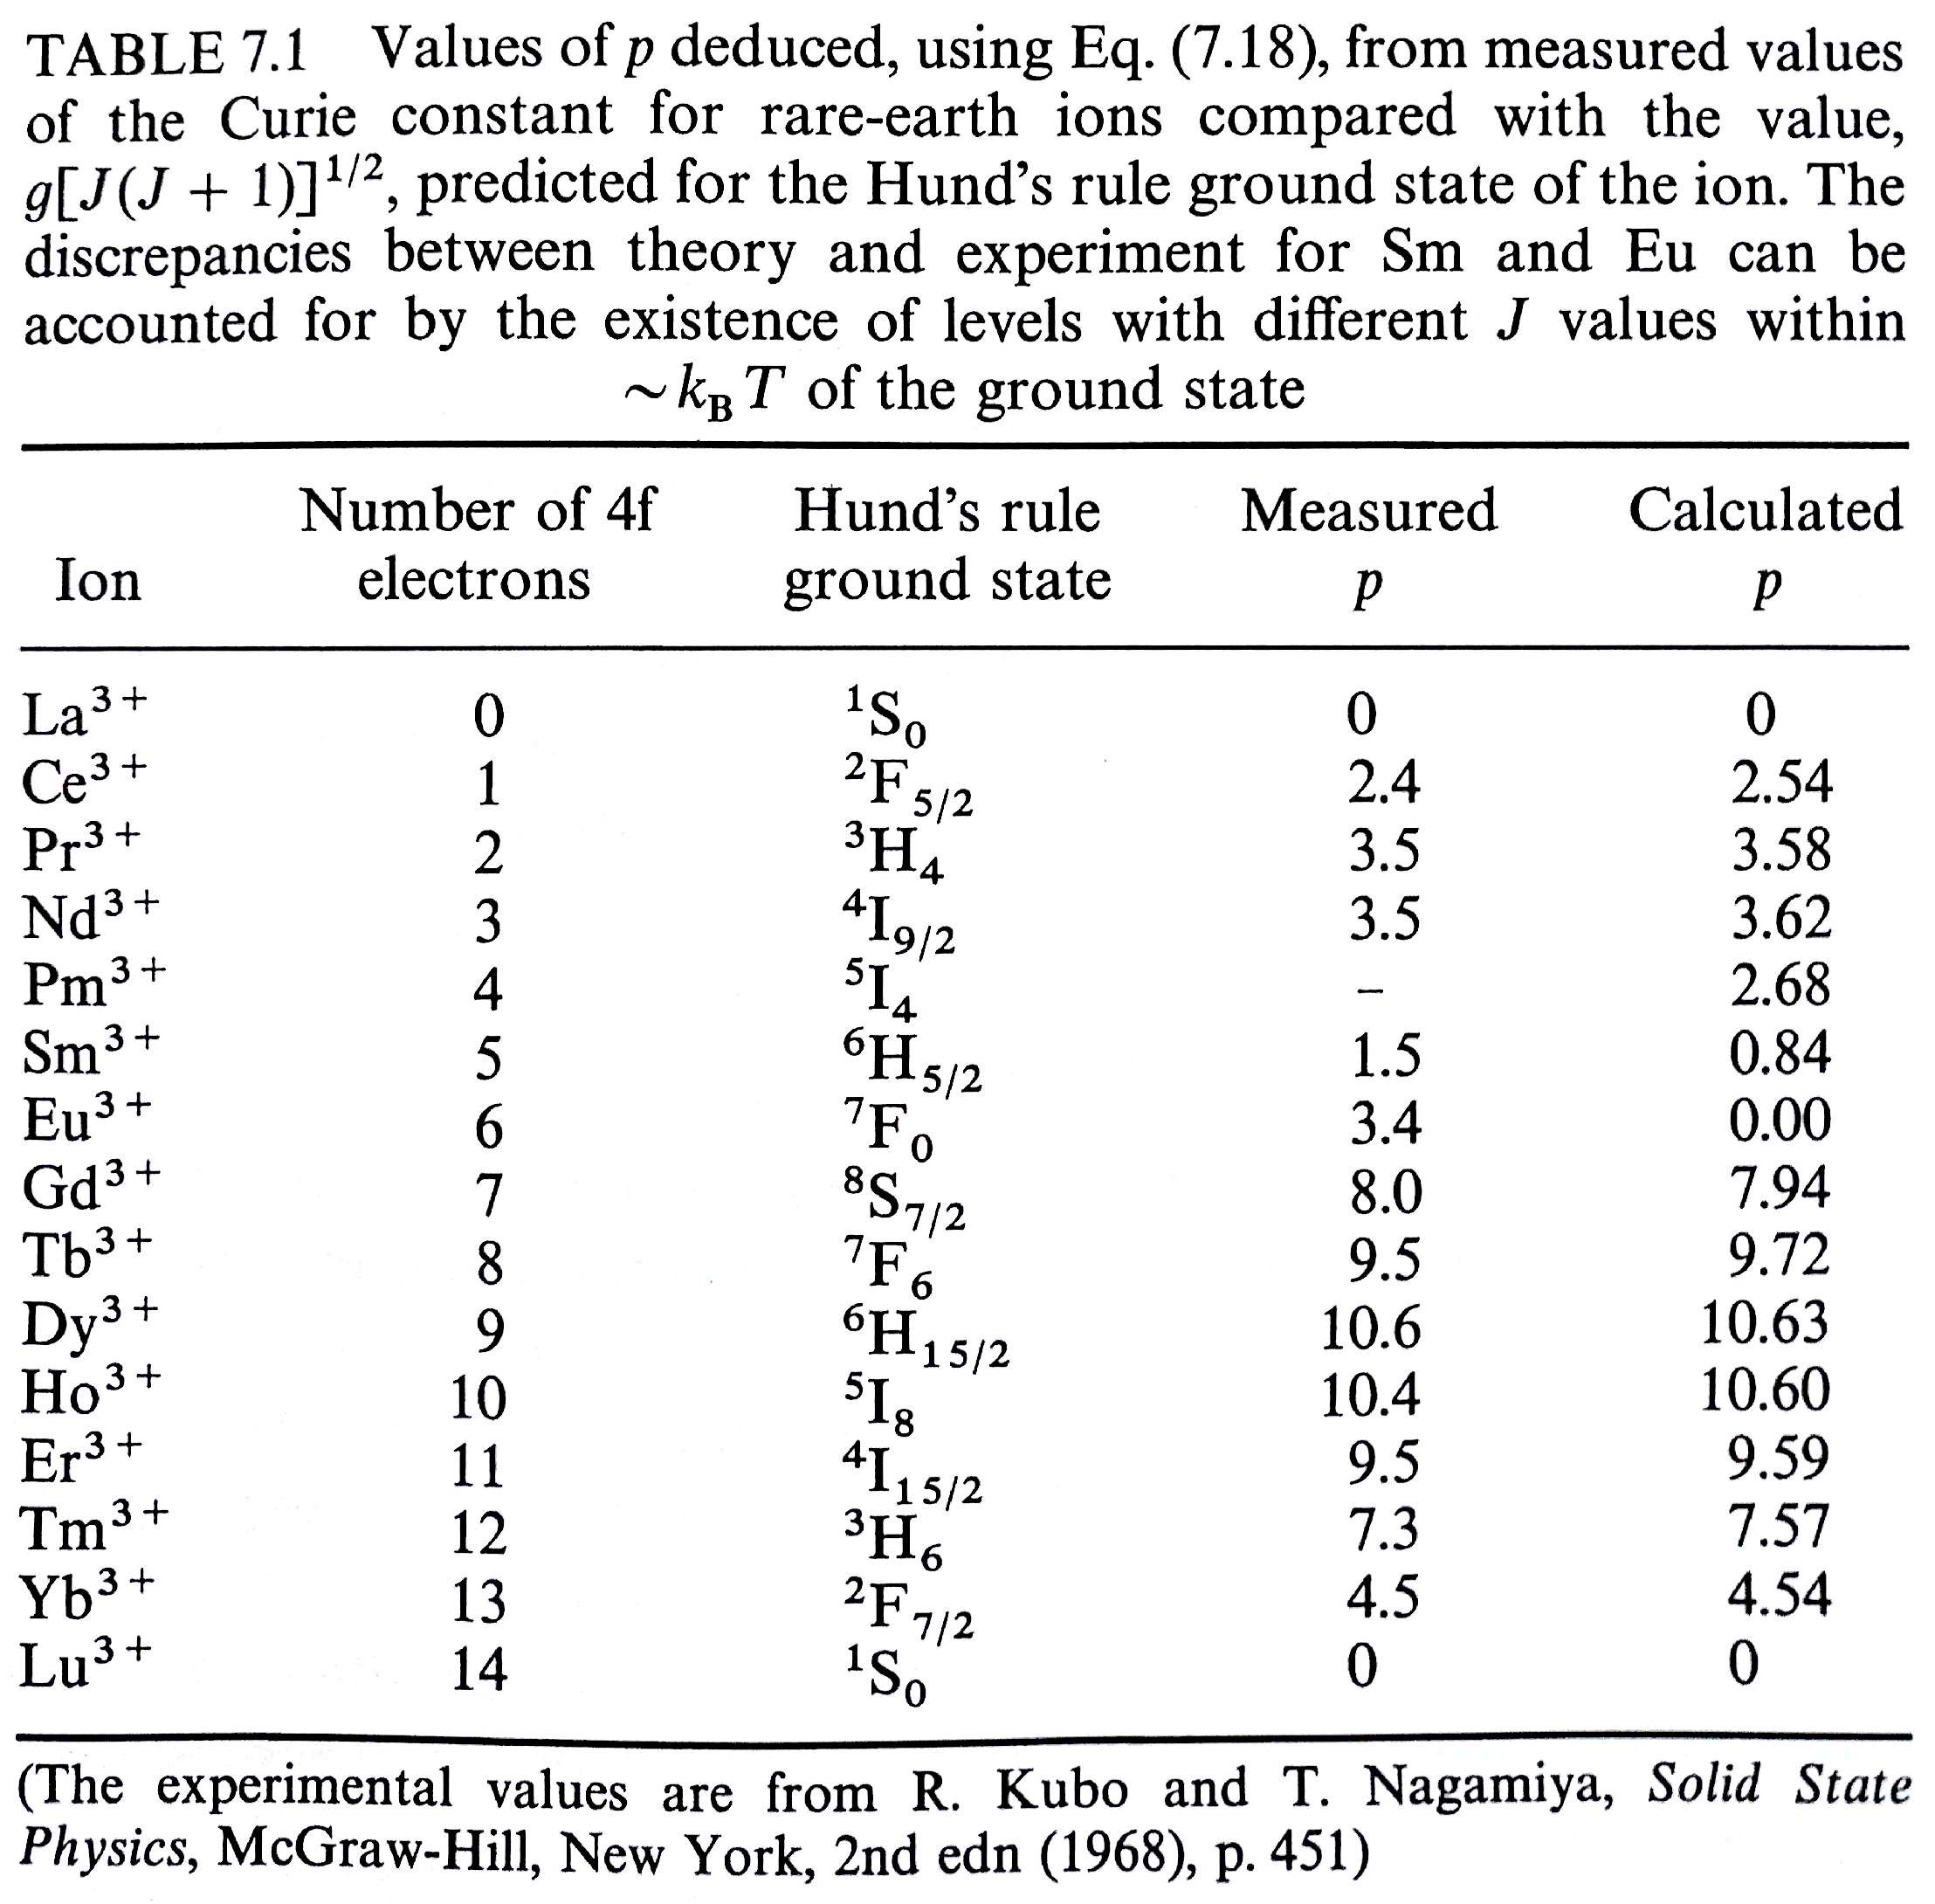
\includegraphics[width=\textwidth]{quench-l}
	\caption{Copied from Solid State Physics by J.R. Hook and H.E. Hall}
	\label{fig:quench-l}
\end{figure}

\begin{figure}[!ht]
	\centering
	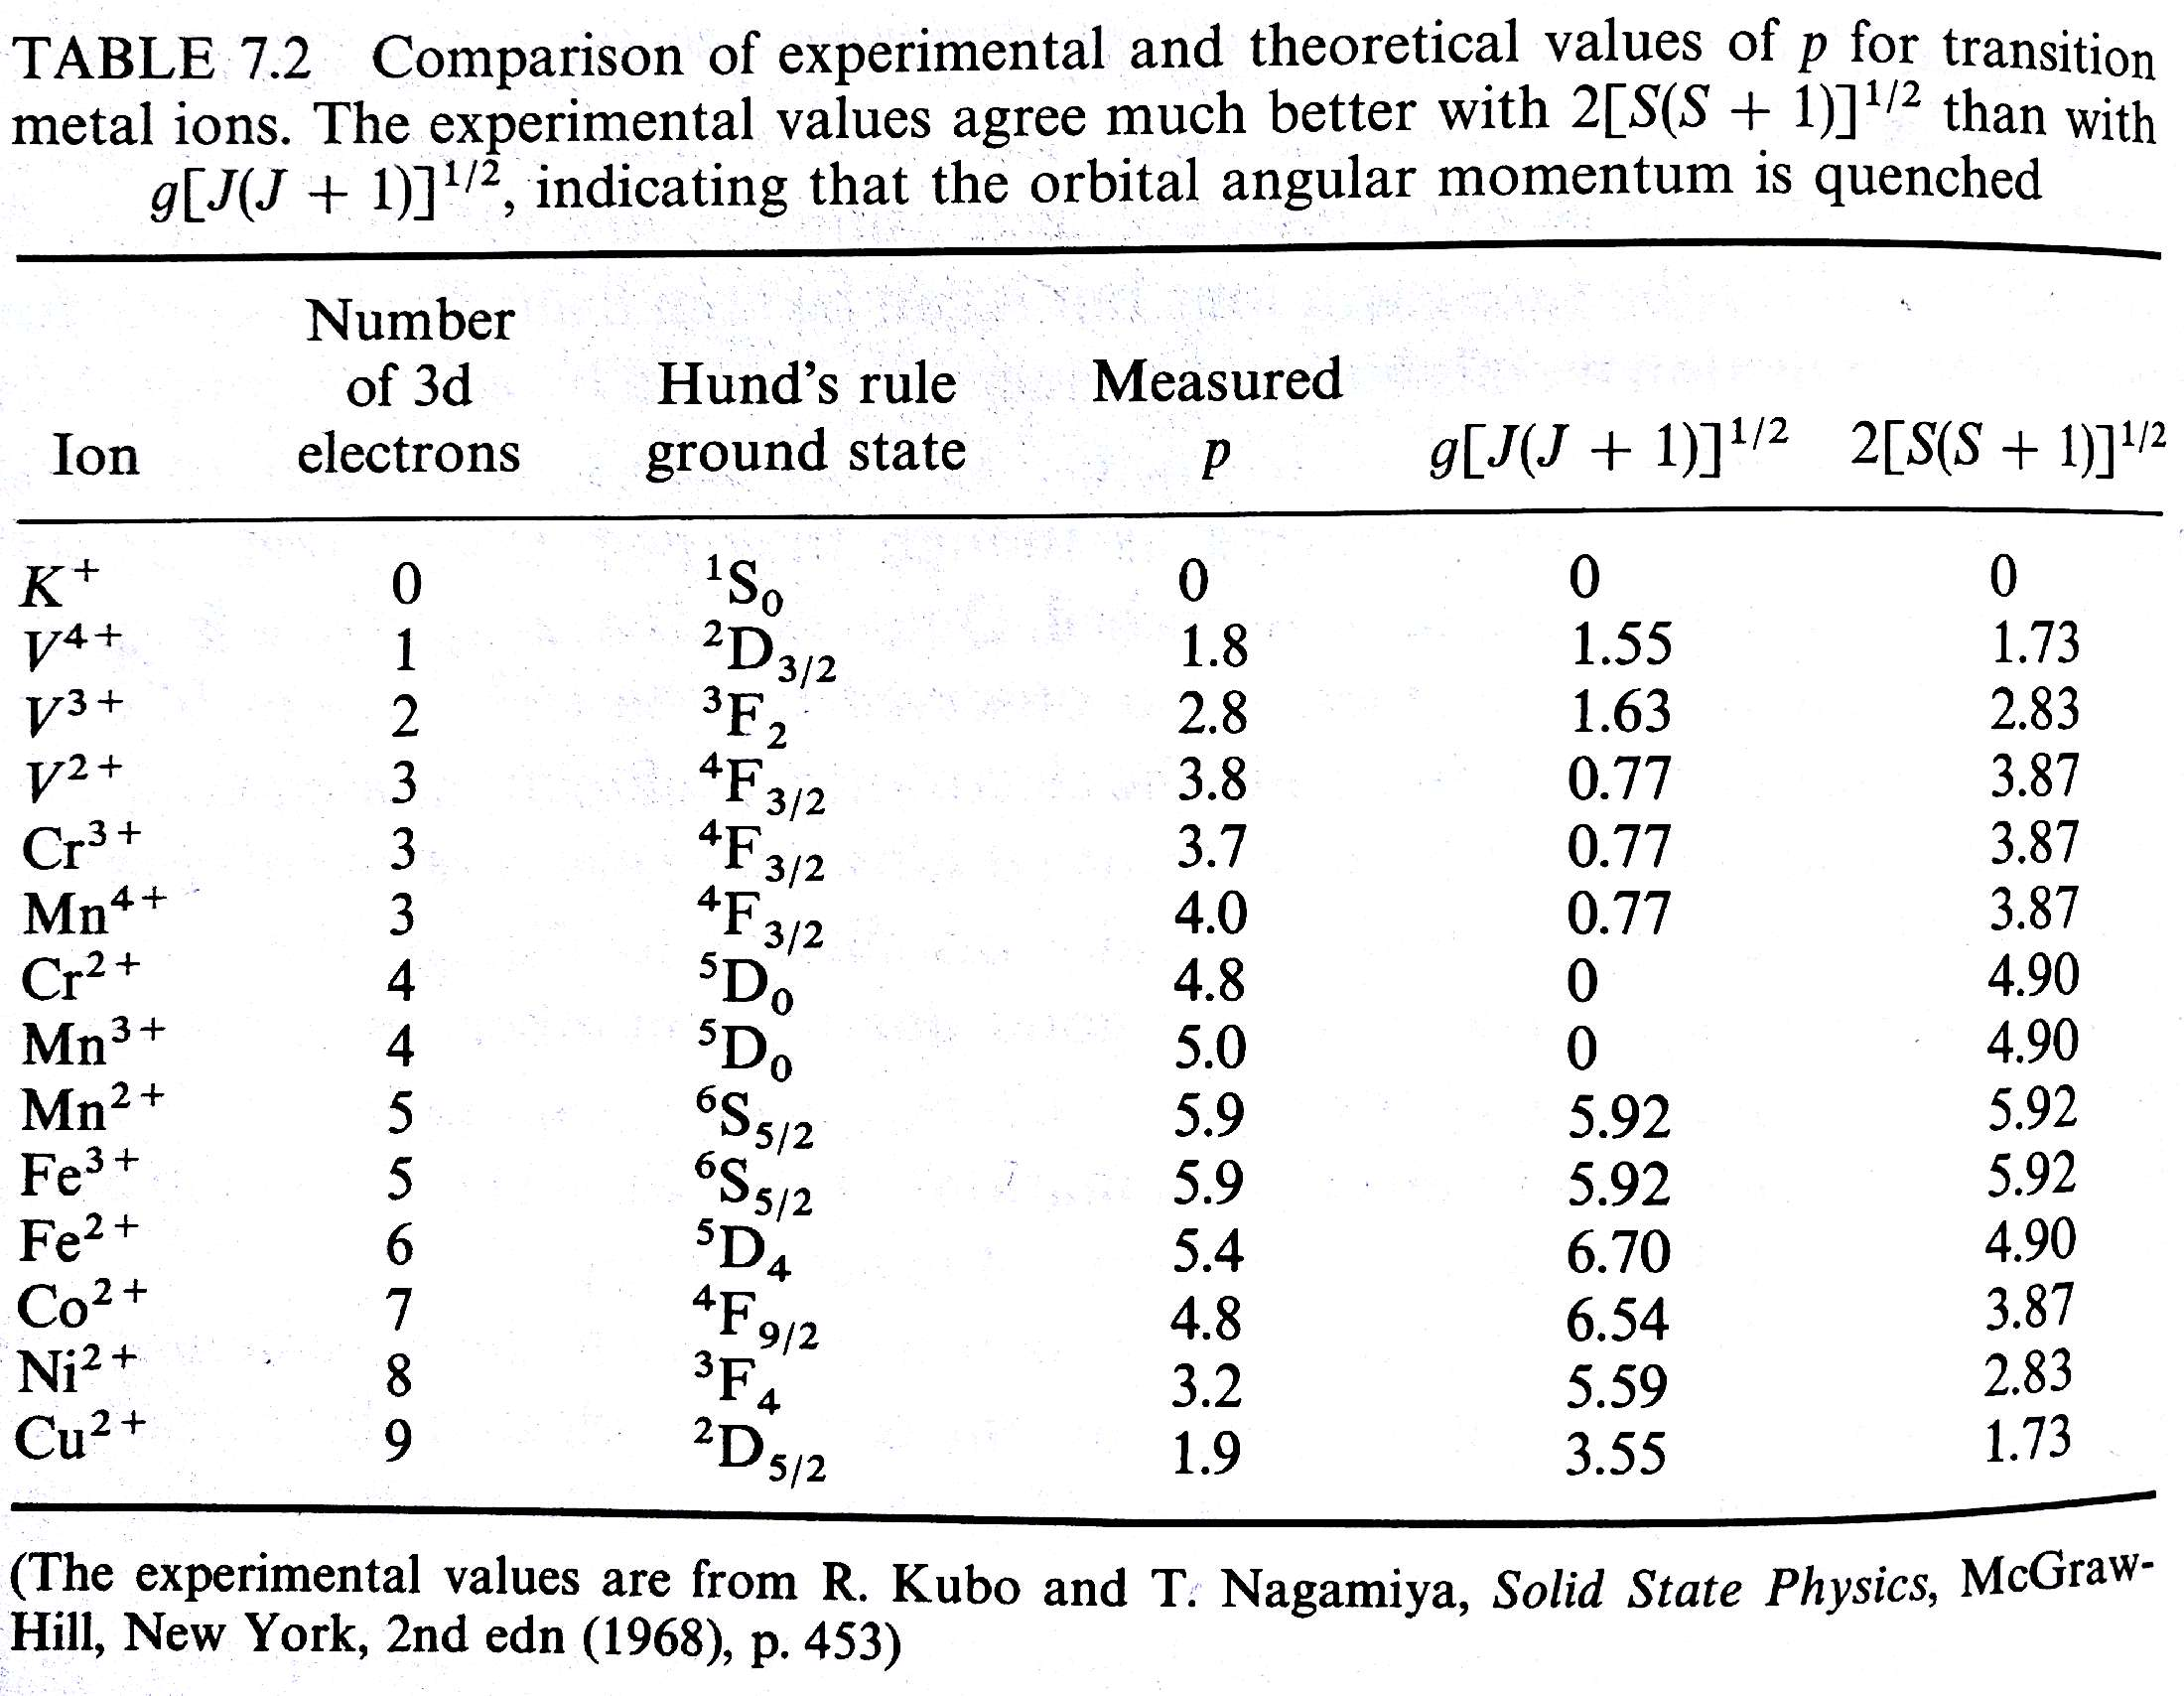
\includegraphics[width=\textwidth]{quench-s}
	\caption{Copied from Solid State Physics by J.R. Hook and H.E. Hall}
	\label{fig:quench-s}
\end{figure}

\newpage
\subsubsection{Conduction electron paramagnetism}
TODO
FINISH THIS WHEN YOU READ CHAPTER 3 ABOUT FREE ELECTRONS.


\newpage
\subsection{Diamagnetic}
In the introduction we mentioned a classical effect that generates a screening effect on a changing magnetic field. However, quantum mechanics gives rise to a tendency, in all matter, to give a stable exclusion of applied fields. To understand that we must consider in detail what happens when a charged particle is accelerated by a changing magnetic field.

\subsubsection{Momentum in a magnetic field}
By going through the example in the book on page 211-213, get get an expression of the momentum of a charged particle, $\pmb{p}$, to be
\begin{equation}
	\pmb{p} = M\pmb{v} + q\pmb{A}
	\label{eq:charged_particle_momentum}
\end{equation}
where $M$ is the mass of the charged particle, $v$ is the velocity, $q$ is the charge and $\pmb{A}$ is the magnetic vector potential the particle lies in. This expression is obtained through classical means and gives us a sense that charged particles gives us a momentum that not only depends on its velocity and mass, but also the magnetic vector potential the charged particle exists in.

We will now use equation~\ref{eq:charged_particle_momentum} with $q \to -e$ and $M \to m$ in subsequent subsections.
\subsubsection{Screening by induced currents}
In the book on page 213-214 an argument is made that the quantum states, as related to momentum, is kind of rigid. It needs allot of energy to get exited to another state. Thus a large applied field is required to excite the electrons in an atom. But if we assume that the field is not strong enough to do that, we can assume that when you apply a field the momentum $\langle \pmb{p} \rangle$ stays constant but the velocity $\langle \pmb{v} \rangle$ changes (As described in the previous section). Using equation~\ref{eq:charged_particle_momentum} we get that the induced velocity is
\begin{equation}
	\pmb{v} = \frac{e\pmb{A}}{m}
\end{equation}
and the resulting current density to be
\begin{equation}
	\pmb{j} = n(-e) \pmb{v} = - \frac{ne^2}{m} \pmb{A}
	\label{eq:atomic_current_density}
\end{equation}
In the book on p. 214 it is shown that the screening effect it small. The characteristic length of the vector potential $\pmb{A}$ is two orders of magnitude larger then the atom itself\footnote{The derivation is made through Maxwell's equations and are quite simple, look at it at your leisure}. 

\newpage
\subsubsection{Calculation of the diamagnetic susceptibility}
Looking at figure~\ref{fig:induced-screening} we see a cylindrical system setup so that the z-axis is parallel to $\pmb{B}$ and the origin at the atom.  $\rho$ is the radius and $B$ is the magnitude of the uniform magnetic field applied. It is given in the book that the uniform field created by this system can be expressed through the vector potential 
\begin{equation}
	\pmb{A} = \pmb{\hat{c}} B \rho/2
\end{equation}
\begin{figure}[!ht]
	\centering
	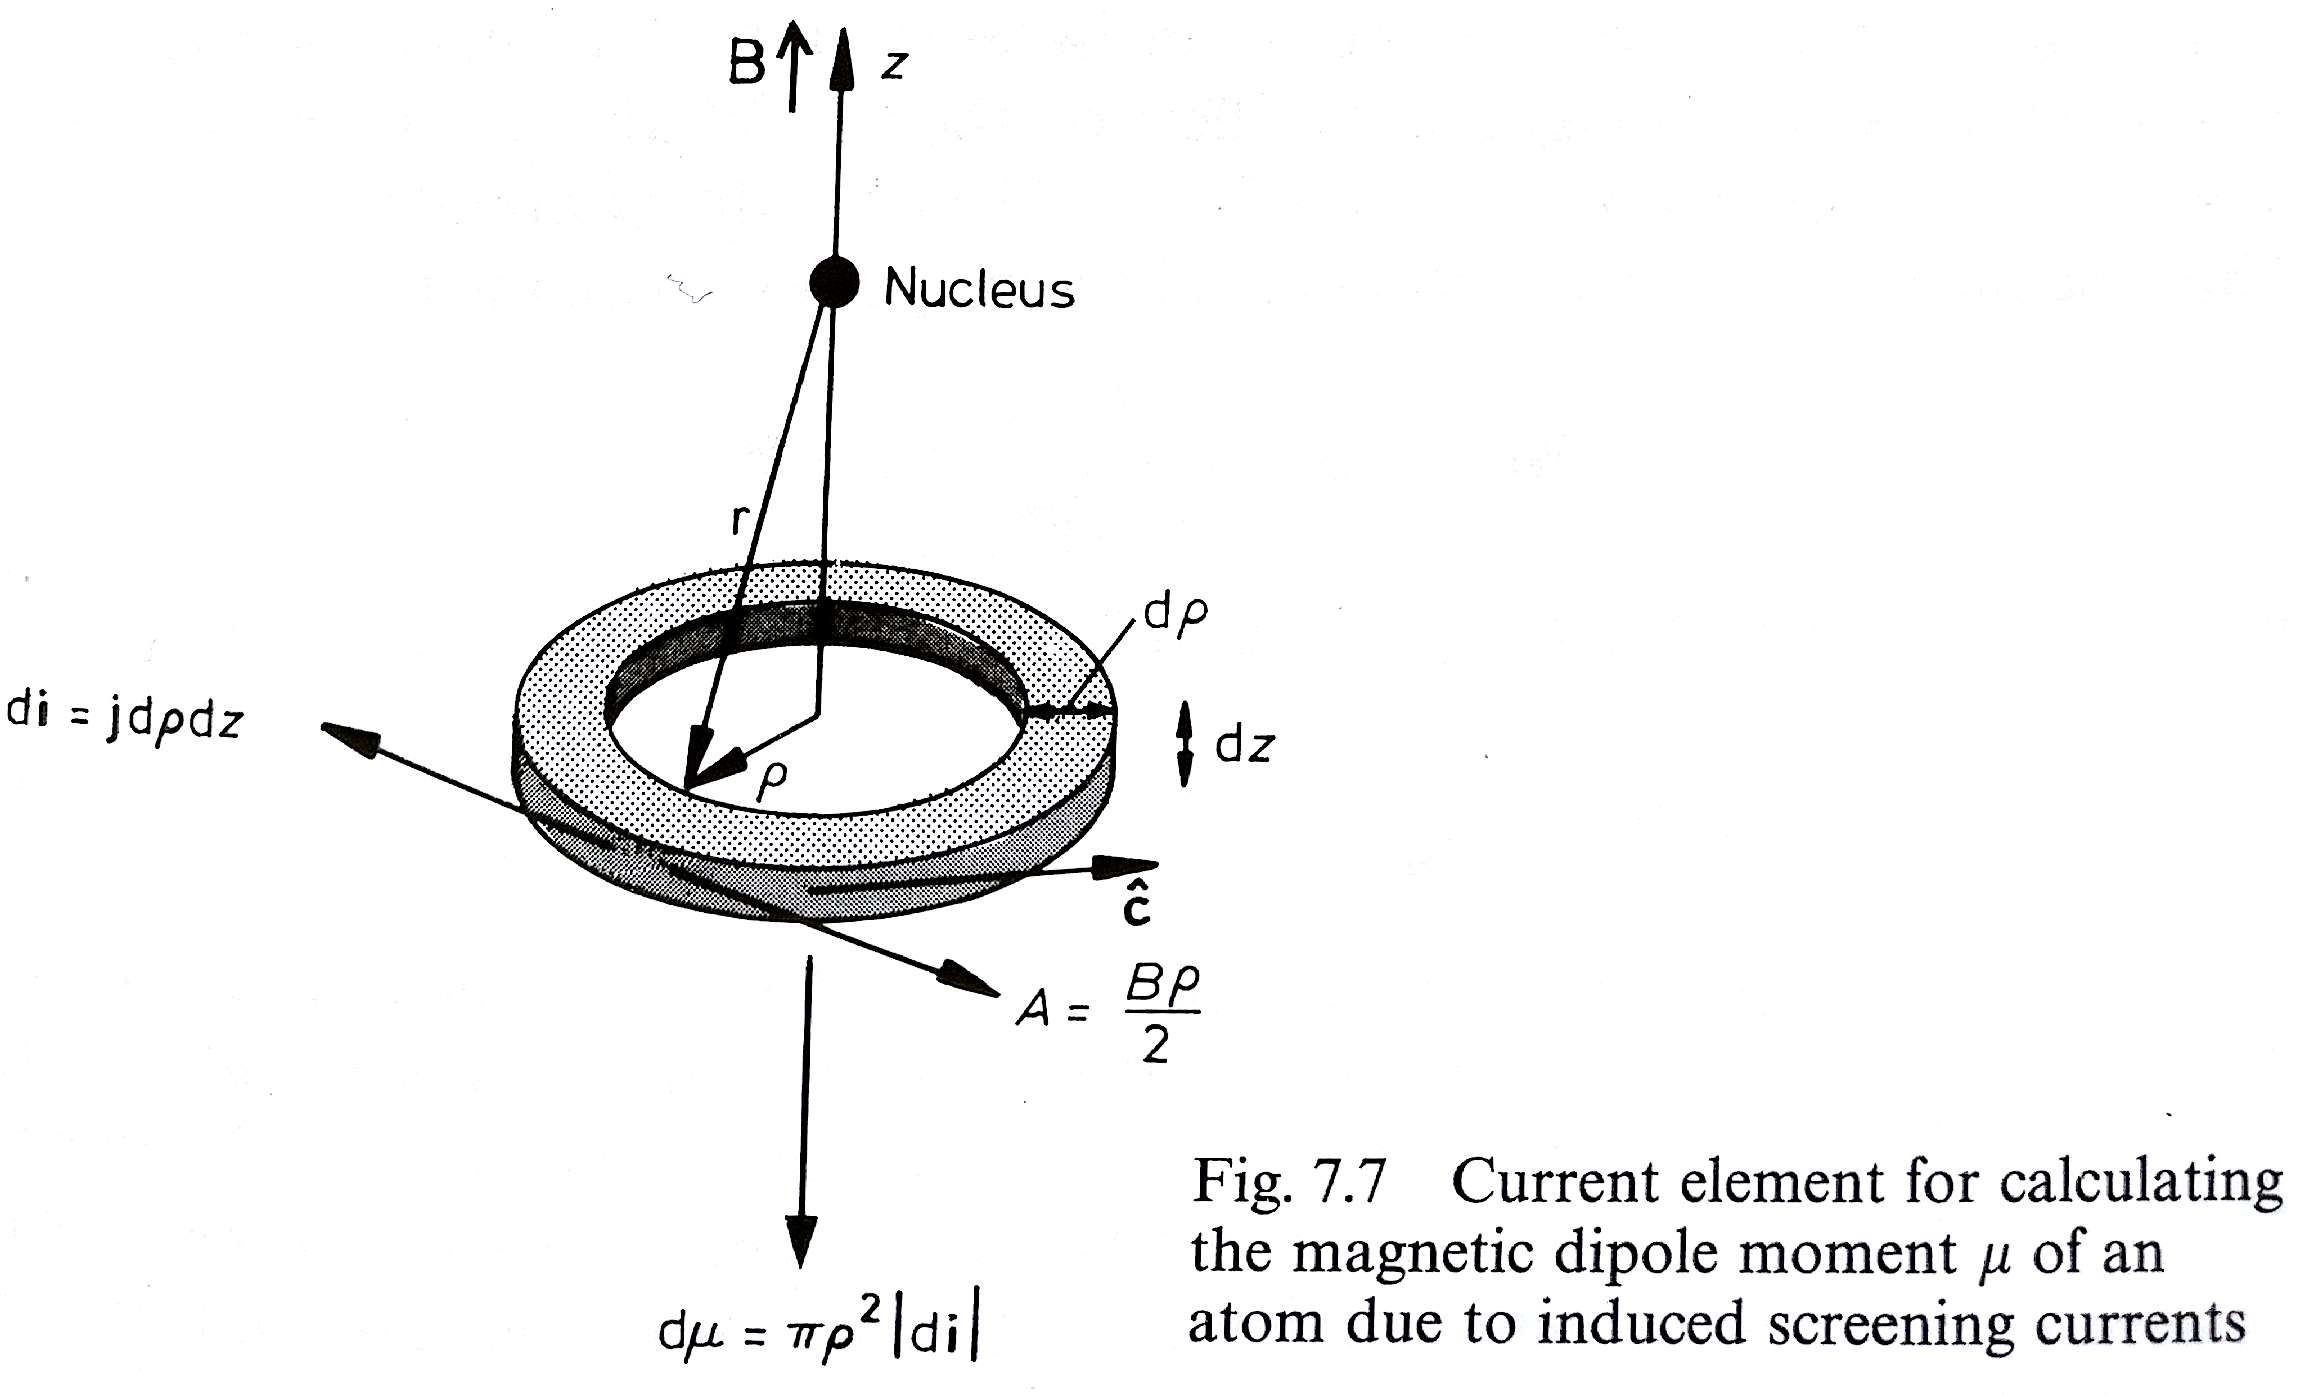
\includegraphics[width=\textwidth]{induced-screening}
	\caption{Copied from Solid State Physics by J.R. Hook and H.E. Hall}
	\label{fig:induced-screening}
\end{figure}
\newpage
thus, by using equation~\ref{eq:atomic_current_density}, the current density becomes\footnote{Note that it's required to have that $div \pmb{A} = 0$ for this vector potential to be usable, otherwise our assumption that $\langle \pmb{p} \rangle$ is constant under the applied field doesn't hold.}
\begin{equation}
	\pmb{j} =  - \pmb{\hat{c}} \frac{ne^2B\rho}{2m}.
\end{equation}
By assuming that $n$ is constant within the ring in figure~\ref{fig:induced-screening}, we can write that the current of this ring $d\pmb{i}$ is
\begin{equation}
	d\pmb{i} = \pmb{j} d\rho dz = - \pmb{\hat{c}} \frac{ne^2B\rho}{2m} d\rho dz
\end{equation}
Using amperes law (equation~\ref{eq:amperes-law}) we get that the ring contributes to the dipole moment, $d\pmb{\mu}$, as
\begin{equation}
	d\pmb{\mu} = - \pmb{\hat{z}} | d\pmb{i} | \pi \rho^2 = -\pmb{B} \frac{e^2\rho}{2m} \pi \rho^2 d\rho dz.
\end{equation}
So the total induced moment becomes
\begin{equation}
	\pmb{\mu} = - \pmb{B} \frac{e^2}{4m} \int n\rho^2 dV
\end{equation}
where $dV = 2\pi d\rho dz$ is the volume of the ring. Since $\int dV = Z$ where $Z$ is the number of electrons in the atom we can write $\int n\rho^2 dV = Z\langle \rho^2 \rangle$, and we get
\begin{equation}
	\pmb{\mu} = - \frac{Z e^2}{4m} \langle \rho^2 \rangle \pmb{B}.
	\label{eq:diamagnetic_dipole_moment}
\end{equation}

Since this effect is weak, we ignore neighbours effect on an ion\footnote{We can then also set $\pmb{B} = \mu \pmb{H}$}. We get the magnetization to be for $N$ such atoms to be
\begin{equation}
	\pmb{M} = N\pmb{\mu} = - \frac{NZe^2}{4m} \langle \rho^2 \rangle \pmb{B}
\end{equation}
using equation~\ref{eq:susceptibility} we get an expression for the susceptibility 
\begin{equation}
	\chi = - \frac{NZe^2 \mu_0}{4m} \langle \rho^2 \rangle \approx 10^{-5}
\end{equation}
Where the approximation in order to the get order of magnitude is done through approximating $\langle \rho^2 \rangle \approx a_0^2$, where $a_0$ is the Bohr radius. A very low susceptibility indeed.
\newpage
\subsection{New words}
\begin{itemize}
	\item \textbf{Diamagnetism}
	\item \textbf{Paramagnetism}
	\item \textbf{Magnetic susceptibility - $\chi$}
	\item \textbf{Magnetization - $\mathbf{M}$}
	\item \textbf{Macroscopic magnetic field within a material - $\mathbf{H}$}
	\item \textbf{Saturation magnetization}
	\item \textbf{Curie law}
	\item \textbf{Curie constant}
	\item \textbf{Quenching}
	\item \textbf{Crystal field}
\end{itemize}

\newpage
\section{Magnetic Order}
\subsection{Introduction}
Spontaneous magnetization occurs without an applied field due to alignment of dipole moments. This usually occurs below temperatures we considered when talking about paramagnets. This is because each dipole somehow gets ``aware'' of each other. When dipoles get ordered the entropy gets lower and we usually talk about three types  of magnetic orders. First the ferromagnetic order, in which all the dipoles are align, then we have the antiferromagnets where all the dipoles get cancelled out and lastly the ferrimagnets where we have a net alignment but there exists dipoles that are turned the opposite way too.

The magnetic interaction is too small to matter\footnote{showed in the book on page 219}. The only power strong enough must be the electrostatic interaction between the electrons. From quantum mechanics we have on such electrostatic interaction which depends on the relative orientation of their magnetic moments, namely the exchange force
\subsection{The exchange interaction}
Wavefunction of two electrons need to be antisymmetric, i.e.
\begin{equation}
	\psi(\pmb{r}_1, \pmb{s}_1:\pmb{r}_2, \pmb{s}_2) = -  \psi(\pmb{r}_2, \pmb{s}_2:\pmb{r}_1, \pmb{s}_1)
\end{equation}
and thus disappears if two electrons where  to occupy the same state. In other words there is no probability that two electrons would be found at the same point in space. Thus this antisymmetry of the wavefunction tends to keep electrons of parallel spin apart, so the expectation energy of the Coulomb repulsion energy $e^2/4\pi \sigma_0 |\pmb{r}_1 - \pmb{r}_2 |$ is lower for electrons with parallel spins then antiparallel spins. 

We represent this exchange interaction as
\begin{equation}
	-2 \mathscr{J} \pmb{s}_1 \cdot \pmb{s}_2
\end{equation}
thus the Coulomb energy is $2\mathscr{J}$ less for parallel spins, as compared to antiparallel spins. This process describes a \emph{direct exchange}. There exists indirect exchange, as described in figure~\ref{fig:indirect-exchange}.
\begin{figure}[!ht]
	\centering
	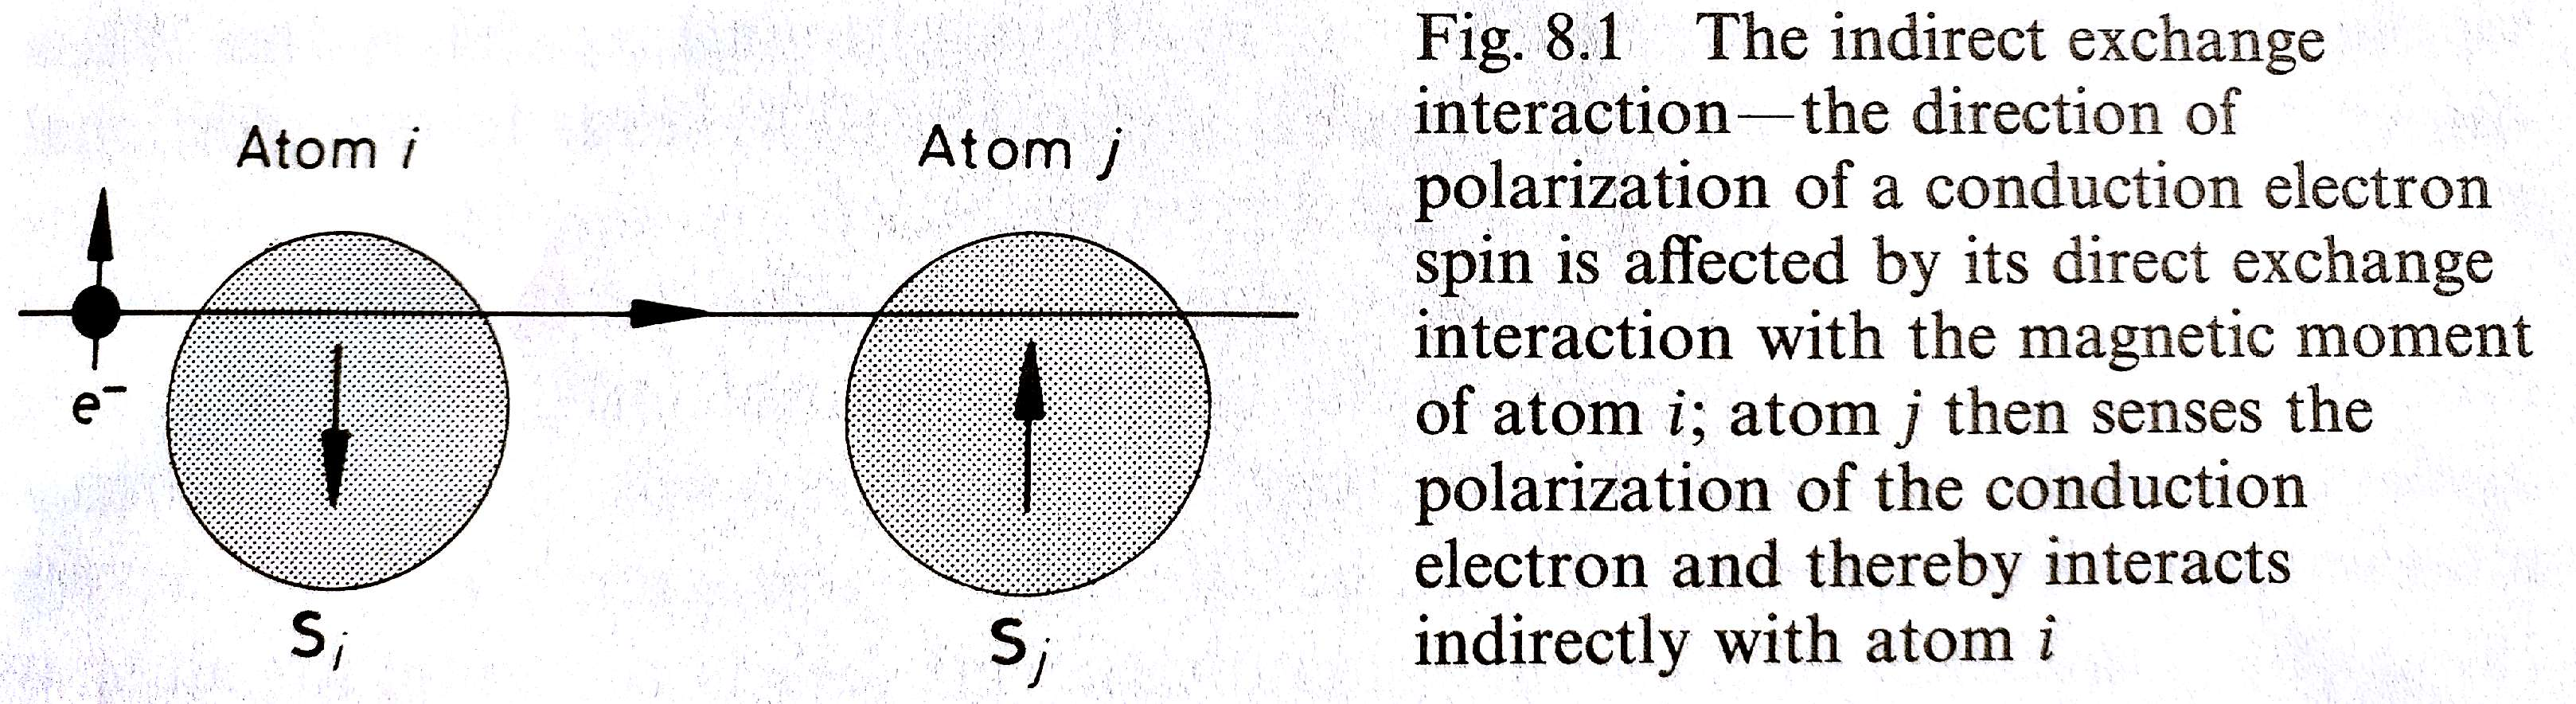
\includegraphics[width=\textwidth]{indirect-exchange}
	\caption{Copied from Solid State Physics by J.R. Hook and H.E. Hall}
	\label{fig:indirect-exchange}
\end{figure}

Well now in reality we have many electrons in an atoms and many atoms in a solid. So if we start with the exchange energy and go on with some dubious assumptions and hypocritical math, we end up with the \emph{Heisenberg Hamiltonian} 
\begin{equation}
	H = - \sum_i \sum_{j \neq i} \mathscr{J}_{ij} \pmb{S}_i \cdot \pmb{S}_j
	\label{eq:heisenberg-hamiltonian}
\end{equation}
where $i$ and $j$ is atoms and $\pmb{S}$ is the \emph{total} angular moment of the specified atom. Please do not confuse this with $\pmb{s}$, the spin. This is basically the $\pmb{J}$ from before. This is the magic sauce we will use to calculate the properties of magnetically ordered materials.

\subsection{Ferromagnetism}
\subsubsection{The Weiss molecular field}
Before quantum mechanics Weiss game around and postulated the existence of a molecular field proportional to the spontaneous magnetization in order to explain spontaneous magnetization. Thus the effective magnetic field acting on any moment was
\begin{equation}
	\pmb{B}_{eff} = \pmb{B}_{loc} + \lambda \mu_0 \pmb{M}
	\label{eq:weiss}
\end{equation}
where $\pmb{B}_{loc}$ is the applied field and $\lambda \mu_0 \pmb{M}$ is the molecular field. Putting in $\pmb{B}_{eff}$ into equation~\ref{eq:alignment_energy} we end up with an additional term $-\lambda \mu_0 \pmb{M}$ in the energy of the dipole moment.

We can approximate equation~\ref{eq:heisenberg-hamiltonian} by assuming that the exchange energy of a particle with total angular momentum $\pmb{S}_i$ can be taken against $\langle \pmb{S} \rangle$ instead of $\pmb{S}_j$\footnote{This calculation is an exercise with hints on page 222}. Through that assumption we can simplify the equation so that we can get the magnetization through equation~\ref{eq:effective-magnetic-moment} to be
\begin{equation}
	\pmb{M} = - Ng \mu_B \langle \pmb{S} \rangle.
\end{equation}
This assumption also leads to a value for the dimensionless constant $\lambda$ in equation~\ref{eq:weiss} to be
\begin{equation}
	\lambda = \frac{2 \sum_{j \neq i} \mathscr{J}_{ij}}{N \mu_0 g^2 \mu_B^2}.
\end{equation}
Thus being proportional to the sum of exchange energies of a spin with all other spins in the solid. This way of approximating spins by their average value, falls into something called mean field theory. 

\subsubsection{Calculation of ferromagnetic properties using the mean field theory}
Using the exact same arguments as we did for the paramagnetic materials earlier but replacing the real magnetic field $\pmb{B}$ with the magnetic field $\pmb{B}_{eff}$ in equation~\ref{eq:paramagnetic-magnetization} with the combination of setting $L=0$, $J=S=\frac{1}{2}$ and $g=2$ for simplicity, we get
\begin{equation}
	M = N\mu_B \\tanh(\frac{\mu_B B_{eff}}{k_B T})
\end{equation}
Which for the high temperature limit $\mu_B B_{eff}/k_B T \ll 1$ becomes\footnote{$\tanh(x) \approx x$}
\begin{equation}
	M = \frac{N \mu_B^2}{k_B T} B_{eff} = \frac{N \mu_B^2}{k_B T} (B_{loc} + \lambda \mu_0 M)
\end{equation}
And here we say that $M$ is proportional to $B_{loc}$, so we have no spontaneous magnetization. Even though we have another term, that just how it is. And we relate the macroscopic field $\pmb{H}$ to the local field $\pmb{B}_{loc}$ through $\mu_0H = B_{loc}$. Thus we get the susceptibility 
\begin{equation}
	\chi = \frac{M}{H} = \frac{C}{T-T_c}
\end{equation}
where 
\begin{equation}
	C = \frac{N\mu_0 \mu_B^2}{k_B}
\end{equation}
and 
\begin{equation}
	T_c = \lambda C
\end{equation}
And $T_c$ represents the upper temperatures at which the material displays ferromagnetic properties.

For a treatment in the lower temperature limit $\mu_B B_{eff}/k_B T \gg 1$ I refer to the book at pages 224-226.

TODO ADD SOMETHING ABOUT FREE ELETRONS IN METAL WHEN READ CHAPTER 3 FREE ELECTRONS

\subsection{The Néel model of antiferromagnetism}
If the exchange energy $\mathscr{J}_{ij}$ is negative the antiparallel alignment is preferred. Thus we have no magnetization. One way to look at this is splitting up the lattice is two different sublattices $A$ and $B$ in which the spins in the $A$ lattice is antiparallel to the spins in the $B$ lattice.

Néel proposed a generalization to the Weiss molecular field  by supposing that the atoms on one sublattice experience a molecular field proportional to the magnetization of the other sublattice and opposite in direction to it. Thus we end up with the equations
\begin{align}
	\pmb{B}^{\pmb{A}}_{eff} &= \mu_0 (\pmb{H} - \lambda \pmb{M}_{\pmb{B}}) \\
	\pmb{B}^{\pmb{B}}_{eff} &= \mu_0 (\pmb{H} - \lambda \pmb{M}_{\pmb{A}})
\end{align}
Which can be obtained from the Heisenberg Hamiltonian(equation~\ref{eq:heisenberg-hamiltonian}) if assumed that only nearest neighbour interactions are important and that all the nearest neighbour of any $A$ moment are from the $B$ sublattice. Doing the same treatment as before we did for ferromagnets, we get two magnetizations
\begin{align}
	M_A &= \frac{N}{2} \mu_B \tanh{(\frac{\mu_B B^A_{eff}}{k_B T})} \\
	M_B &= \frac{N}{2} \mu_B \tanh{(\frac{\mu_B B^B_{eff}}{k_B T})}
\end{align}
Once again we look at the high temperature limit and end up with the result\footnote{for details look at page 230 in book}
\begin{equation}
	M = M_A + M_B = \frac{C}{T + \lambda C/2} H
\end{equation}
with 
\begin{equation}
	\lambda = - \frac{4z \mathscr{J}}{N \mu_0 g^2 \mu^2_B}.
\end{equation}
Note that $\mathscr{J}$ is negative so $\lambda$ is positive. $C$ is the curie constant from the section of ferromagnetics. The susceptibility then becomes
\begin{equation}
	\chi = \frac{M}{H} = \frac{C}{T+ T_N}
\end{equation}
where 
\begin{equation}
	T_N = \lambda C/2
\end{equation}

The big difference here is that below the Néel temperature ($T_N$) the susceptibility gets very low. Thus goes into an ordered state with no magnetization. It also matters if the applied field is parallel or perpendicular to the lattice. This further explained on page 231 of the book.

\newpage
\subsection{Ferromagnetic Domains}
Despite the spontaneous magnetization, macroscopic samples of ferromagnetic materials usually have a negligible total dipole moment in the absence of an applied field. Usually have a negligible total dipole moment in the absence of an applied field. This is because such materials often consist of small regions, called domains, which magnetization points in different directions. In figure~\ref{fig:domains} we can see this effect in a 50 $\mu m$ crystal of iron. The seemingly sharp walls which separates the domains are called \emph{Block walls}. These walls are depicted in figure~\ref{fig:bloch-wall} and as we can see they are not in fact sharp, but a smooth transition.

\subsubsection{The energy and thickness of a Bloch wall}
To look at the energy of a bloch wall we need to look at the change in exchange energy due to the variation of the magnetization in the bloch wall. We assume the spins lie on a simple cubic lattice of side $a$ and assume there is a domain wall of the form in figure~\ref{fig:bloch-wall} in the xy-plane. We then end up with an expression\footnote{haphazardly derived in pages 247-249 in the book} for the wall energy per unit area to be
\begin{equation}
	\sigma = \pi a (\frac{WK}{3})^{1/2}
\end{equation}
and a wall thickness 
\begin{equation}
	t = \pi a (\frac{W}{3K})^{1/2}
\end{equation}
where $K$ is a constant given in the book without explanation, and $W$ is the exchange energy per unit volume
\begin{equation}
	W = \frac{6\mathscr{J} s^2}{a^3}
\end{equation}
Basically the point of this derivation was to show that the Bloch wall is about a 100 atoms thick and much higher energy than a region of uniform magnetization. Thus we need to explain why these domains would occur since there is so much energy associated with the walls themself. 

\newpage
\begin{figure}[!ht]
	\centering
	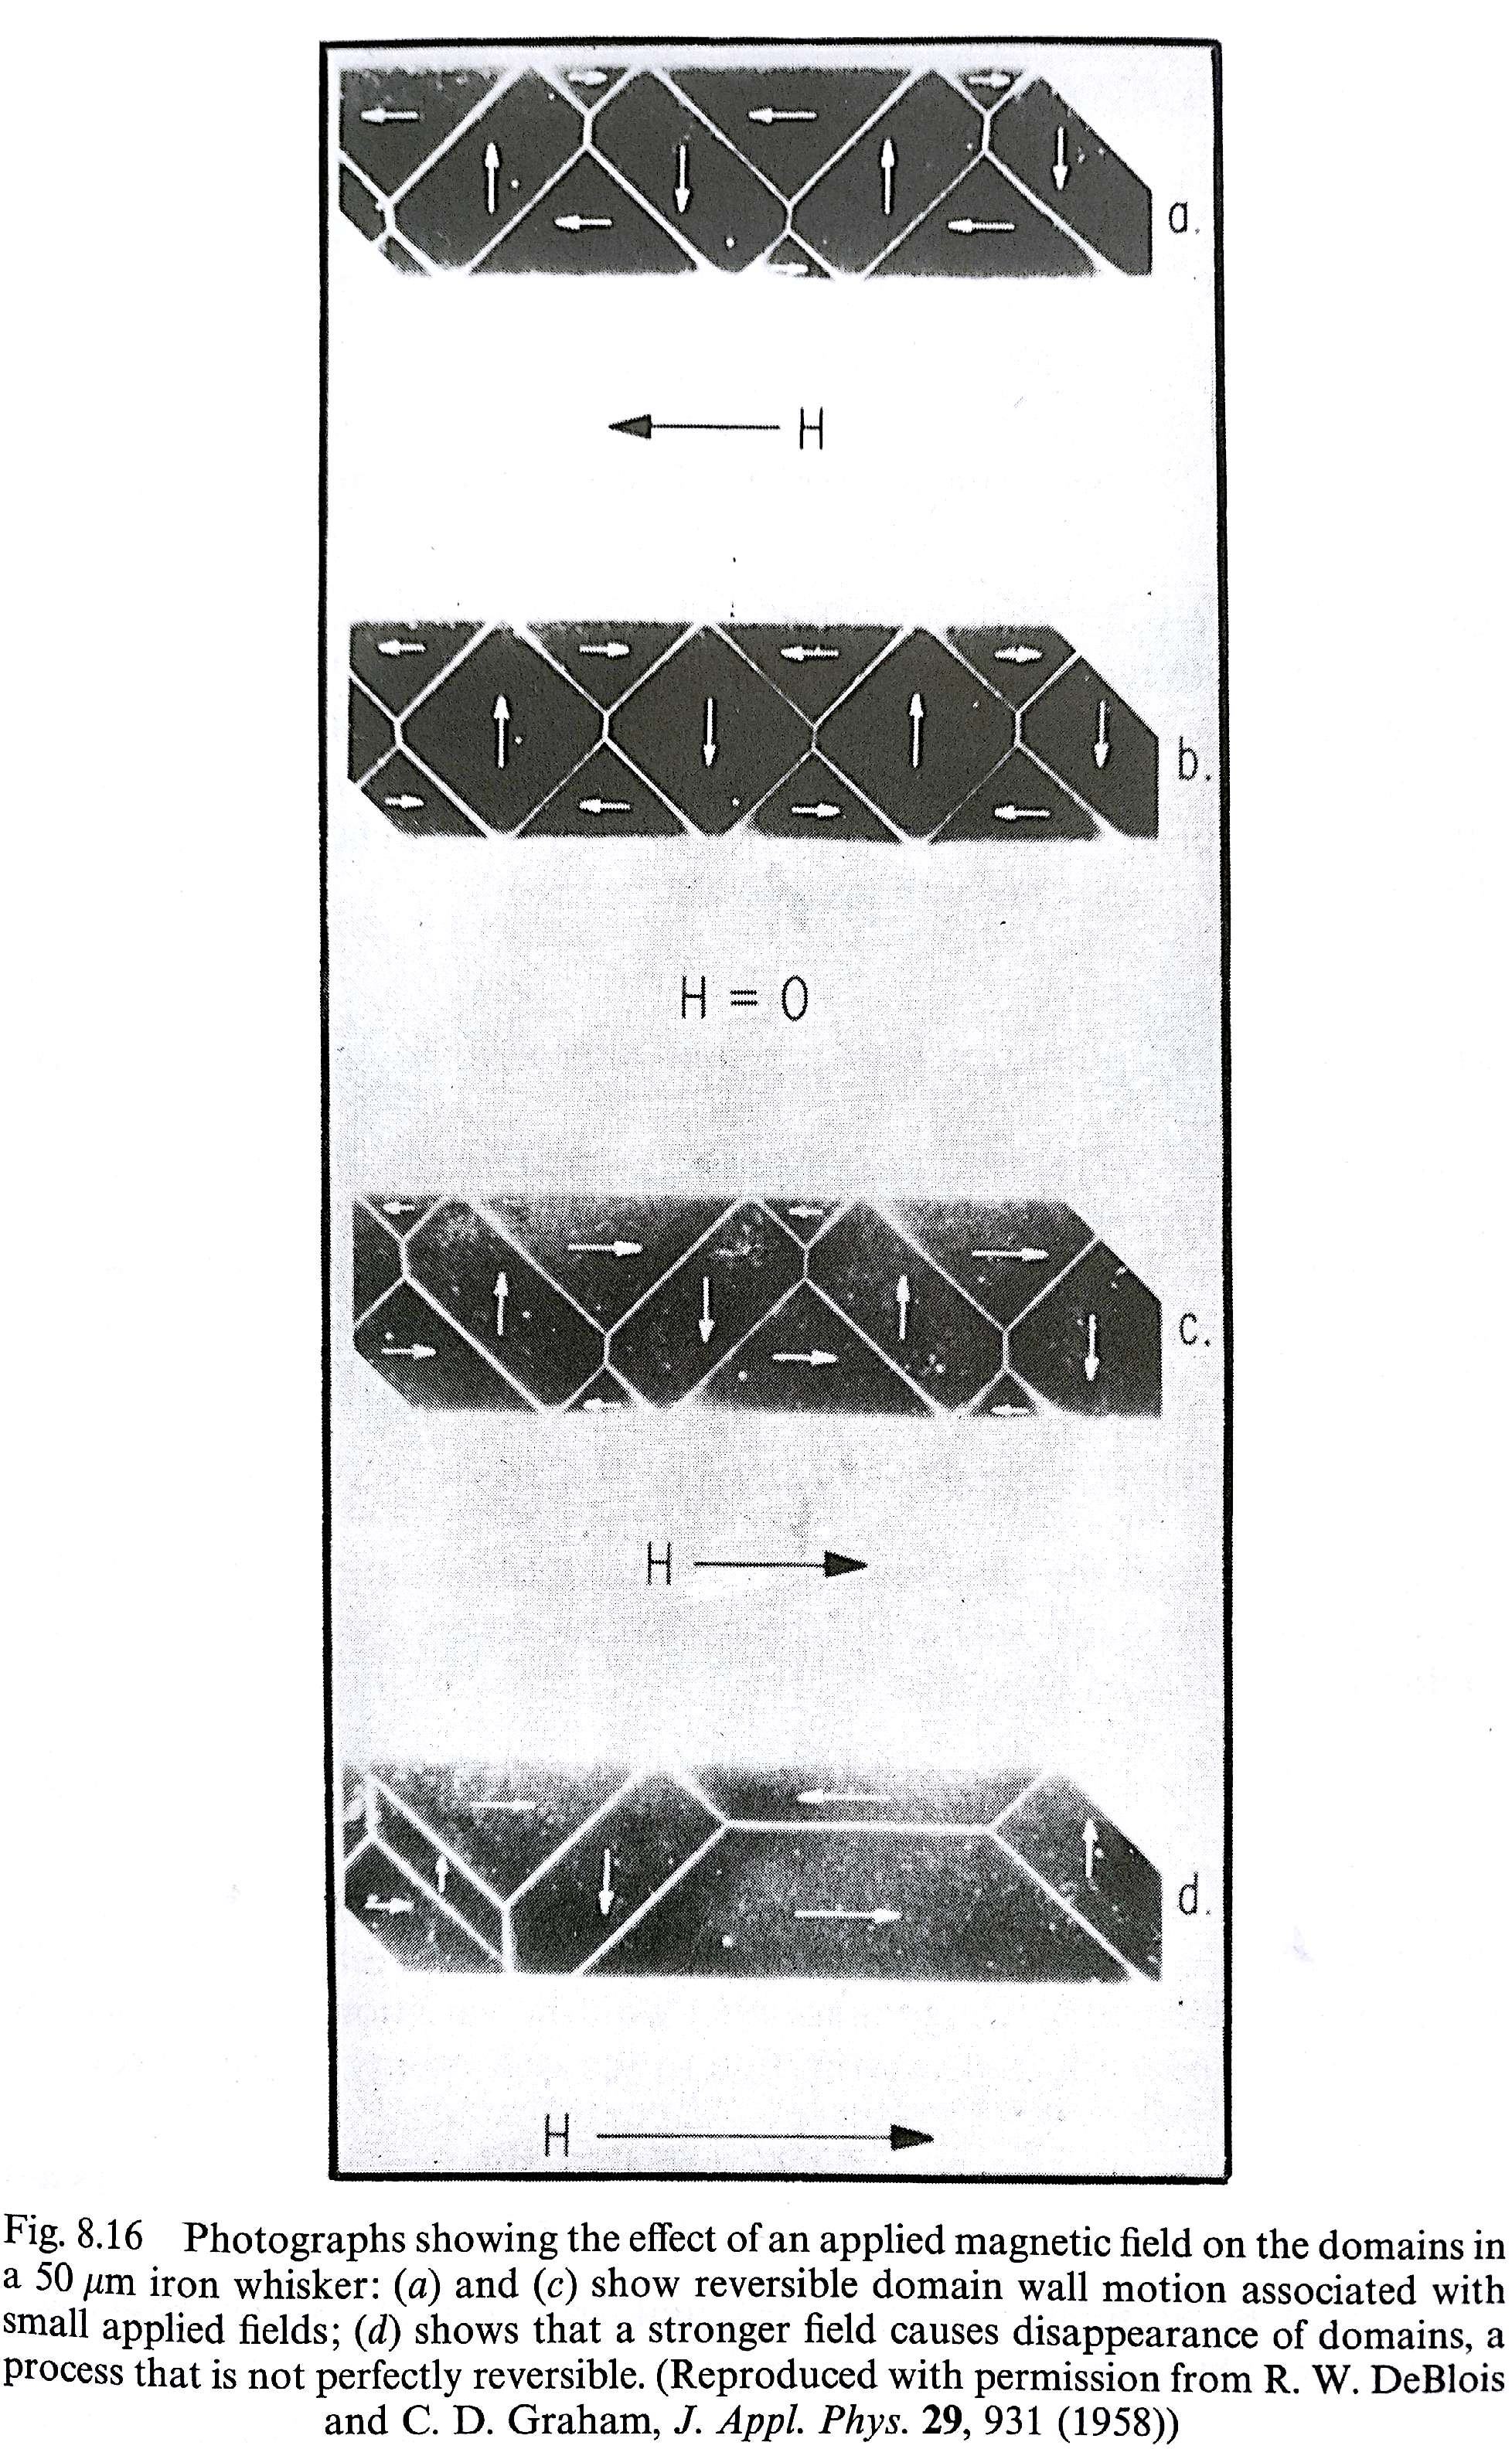
\includegraphics[width=0.8\textwidth]{domains}
	\caption{Copied from Solid State Physics by J.R. Hook and H.E. Hall}
	\label{fig:domains}
\end{figure}
\newpage

\begin{figure}[!ht]
	\centering
	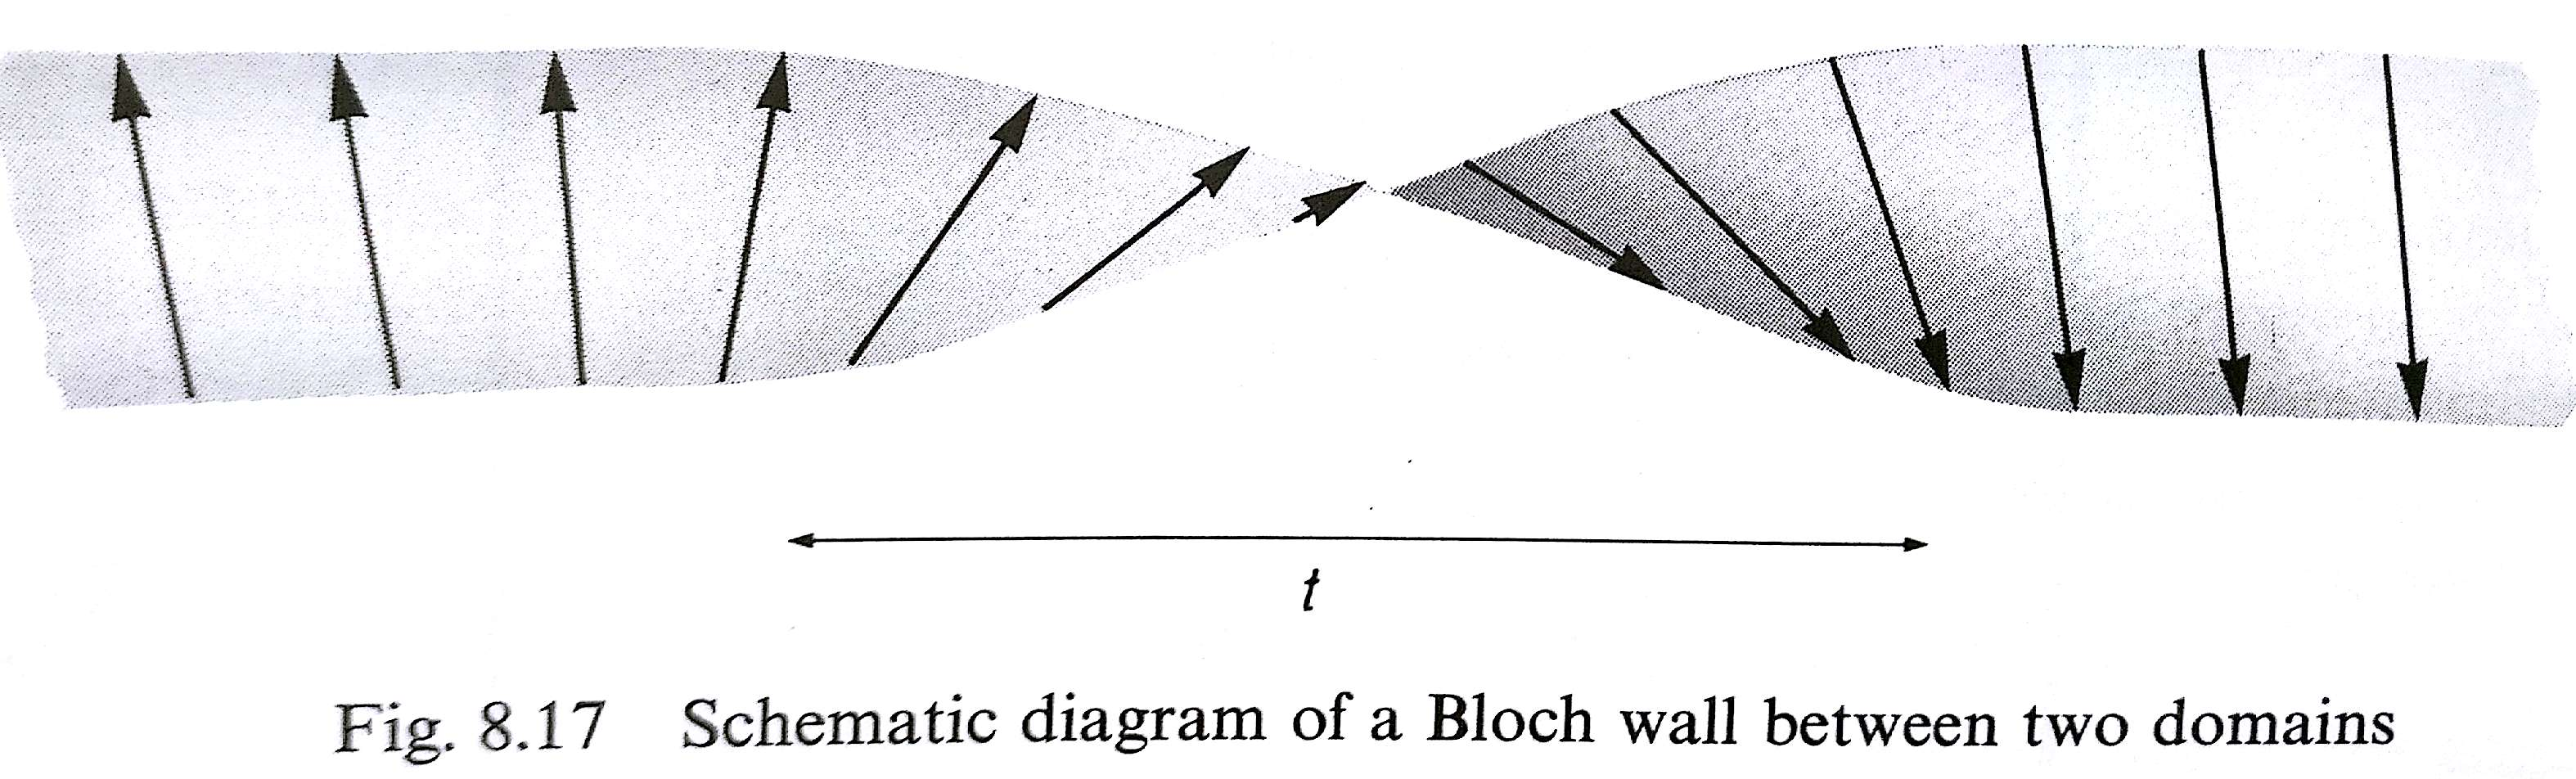
\includegraphics[width=\textwidth]{bloch-wall}
	\caption{Copied from Solid State Physics by J.R. Hook and H.E. Hall}
	\label{fig:bloch-wall}
\end{figure}

\newpage
\subsubsection{Why do domains occur?}
Basically there is a large amount of energy associated with magnetic field outside the crystal\footnote{$B^2/2\mu_0$ per unit volume!}, looking at figure~\ref{fig:domains-occur} we can see how much smaller this magnetic fields becomes if we subdivide the material into domains. So basically the there is a balance for the least amount of energy where the bloch wall energy and the magnetic field energy outside the crystal is minimized. Beyond this the structure of the domains might be weird on first look. This is due to \emph{magnetostriction}. Basically a magnetized crystal tends to expand or contract along the magnetization direction. This magnetostriction creates a stress energy, so this is also taken into account to as something that want to be minimized.

\begin{figure}[!ht]
	\centering
	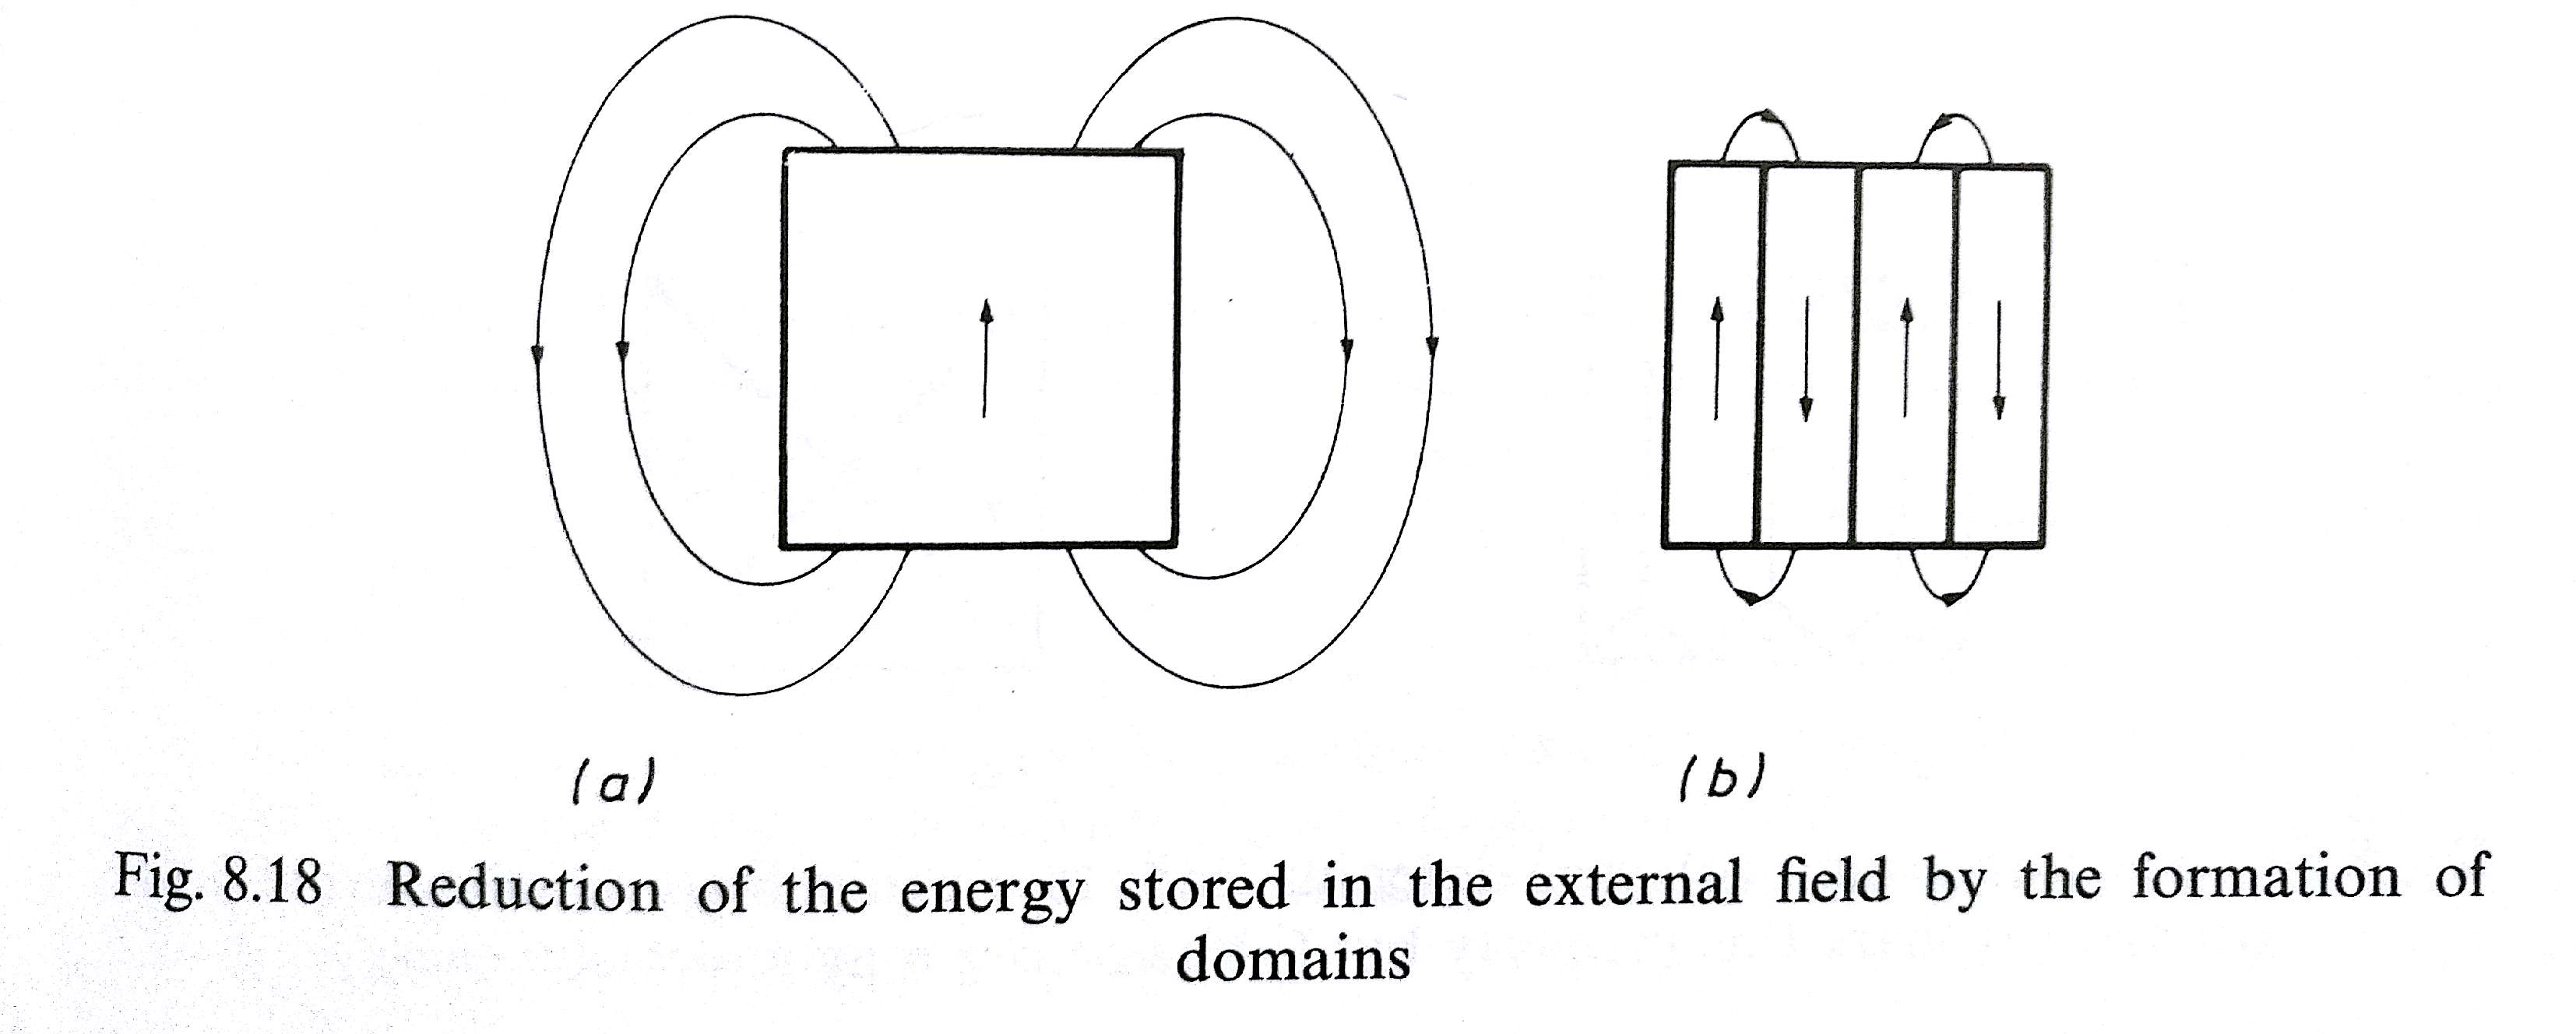
\includegraphics[width=\textwidth]{domains-occur}
	\caption{Copied from Solid State Physics by J.R. Hook and H.E. Hall}
	\label{fig:domains-occur}
\end{figure}

\begin{figure}[!ht]
	\centering
	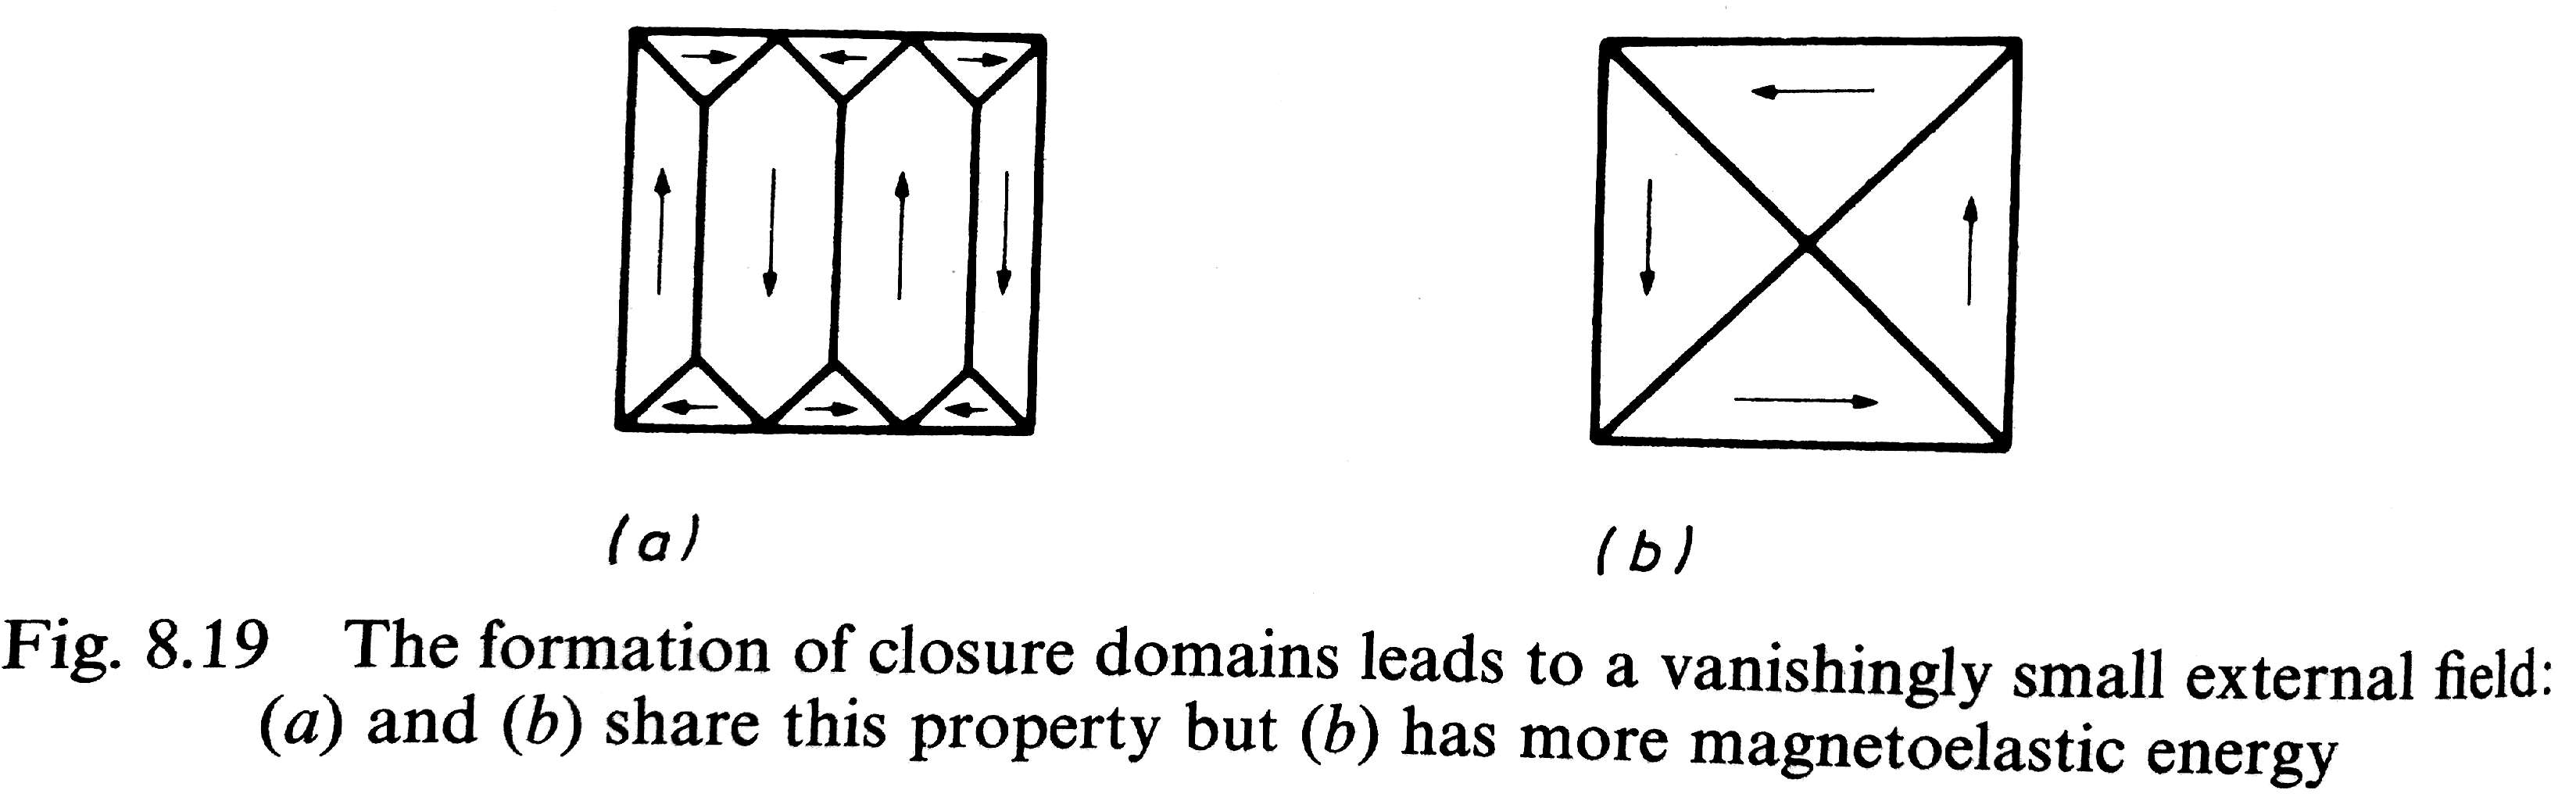
\includegraphics[width=\textwidth]{domain-structure}
	\caption{Copied from Solid State Physics by J.R. Hook and H.E. Hall}
	\label{fig:domain-structure}
\end{figure}

\subsubsection{Magnetization curves of ferromagnets}
Basically the domains can be broken by a large applied field and it taking to much energy to go back to lower energy state, thus creating permanent magnets. For more information I refer to pages 250-251 of the book.


\newpage
\subsection{New words}
\begin{itemize}
	\item \textbf{Magnetic order}
	\item \textbf{Ferromagnetism}
	\item \textbf{Bloch wall}
	\item \textbf{Mean field theory}
	\item \textbf{Spontaneous magnetization}
	\item \textbf{Ferromagnetic order}
	\item \textbf{Antiferromagnets}
	\item \textbf{Ferrimagnets}
	\item \textbf{Heisenberg Hamiltonian}
	\item \textbf{Molecular field}
	\item \textbf{Mean field theory}
	\item \textbf{Magnetostriction}
	\item \textbf{}
	\item \textbf{}
\end{itemize}
\newpage

\section{Crystal dynamics + some more Waves in Crystals}
\subsection{Introduction}
The idea that every atom has a fixed point in a lattice structure with a basis is not a complete picture of solids. It would be waay too easy if that where the case. No, atoms vibrate around their equilibrium position. In fact, we cannot know bot the position and momentum of a particle, due to the Heisenberg uncertainty principle. So even at absolute zero temperature, the atoms possesses a \emph{zero point energy} which causes their \emph{zero point motion}, or vibration around their equilibrium position. At higher temperature this vibration of course gets larger and these motions are often referred to as \emph{lattice vibrations}. 

We will start with calculating under the assumption that the lattice vibrations are of very small amplitudes. Thus the solid is close to a position of stable equilibrium and we can estimate the vibrations through the simple harmonic oscillator\footnote{To the rescue again!}.

We need to figure out the wavefunctions and energies of the electrons within a crystal in order to get a complete picture of the vibrations, luckily we get many important properties without these calculations.
\subsection{Sound waves}
In pages 34-35 of the book we get a derivation of sound waves through a solid. Important assumptions is that $\delta x$ (the displacement in the solid considered) caused by the sound wave, is both much larger then the atomic spacing $a$ and much smaller then the wavelength of the sound wave. The derivation ends up with equation
\begin{equation}
	\frac{C}{\rho} \frac{\partial^2 \xi}{\partial x^2} = \frac{\partial^2 \xi}{\partial t^2}.
\end{equation}
Thus giving the sound wave the speed
\begin{equation}
	v_L = \sqrt{\frac{C}{\rho}}
\end{equation}

\subsection{Lattice vibrations of one-dimensional crystal}
\subsubsection{Chain of identical atoms}
To solve for the displacement of the atoms in a 1d crystal as depicted in figure~\ref{fig:1d-crystal} we look at the Lennard-Jones potential and use the amazing Taylor expansion, thus the problem reduces, as many other problems, to solving for a spring connected line of atoms as depicted in figure~\ref{fig:springs}. We then get the equation 
\begin{equation}
	M \frac{d^2 u_n}{dt^2} = K(u_{n+1} - 2u_n + u_{n-1})
\end{equation}
Where $M$ is the mass of the atom and $K$ is the second derivate of the Lennard-Jones potential evaluated at equilibrium. We then substitute 
\begin{equation}
	u_n = A e^{i(kx^0_n - \omega t)}
\end{equation}
where $x^0_n = na$ is the undisplaced position of the nth atom. Doing this we end up with the equation 
\begin{equation}
	\omega^2 M = 4K \sin^2{(\frac{ka}{2})}
\end{equation}
We apply the periodic boundary condition $u_n =  u_{N+n}$ and note that there should be an integral number of wavelengths is the length of our ring of atoms. Thus we get
\begin{equation}
	Na = p\lambda
\end{equation}
where $p$ is an integer. $k$ then becomes 
\begin{equation}
	k = \frac{2 \pi}{\lambda} = \frac{2\pi p}{Na}
\end{equation}
Thus there is N possible k values in the range $2\pi/N$, the same as we have atoms in the ring of atoms. If one look at the long-wavelength limit $ka \ll 1$ the book shows on page 40 how this result becomes the same as the one previously derived in the previous subsection.
\begin{figure}[!ht]
	\centering
	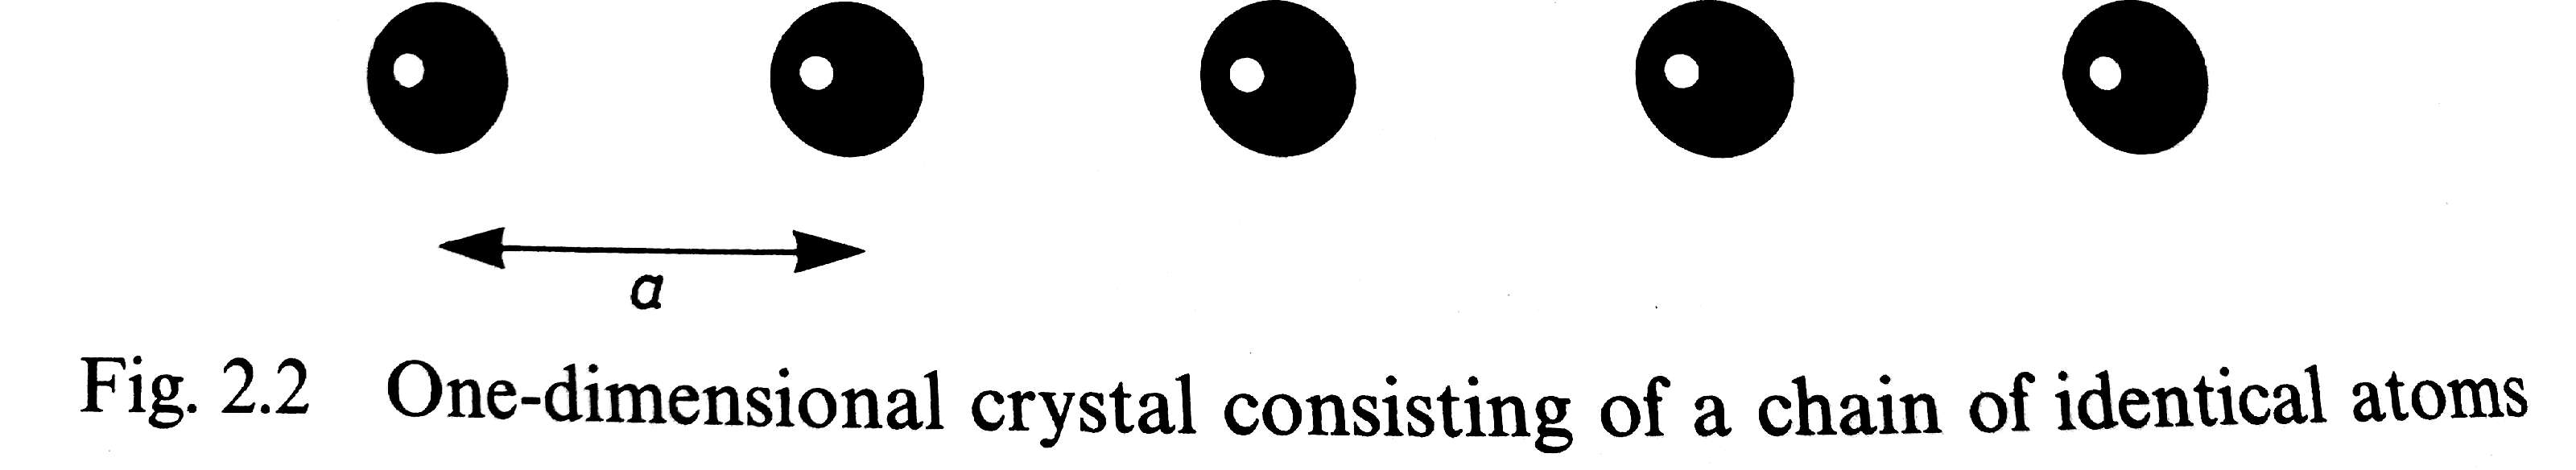
\includegraphics[width=\textwidth]{1d-crystal}
	\caption{Copied from Solid State Physics by J.R. Hook and H.E. Hall}
	\label{fig:1d-crystal}
\end{figure}
\begin{figure}[!ht]
	\centering
	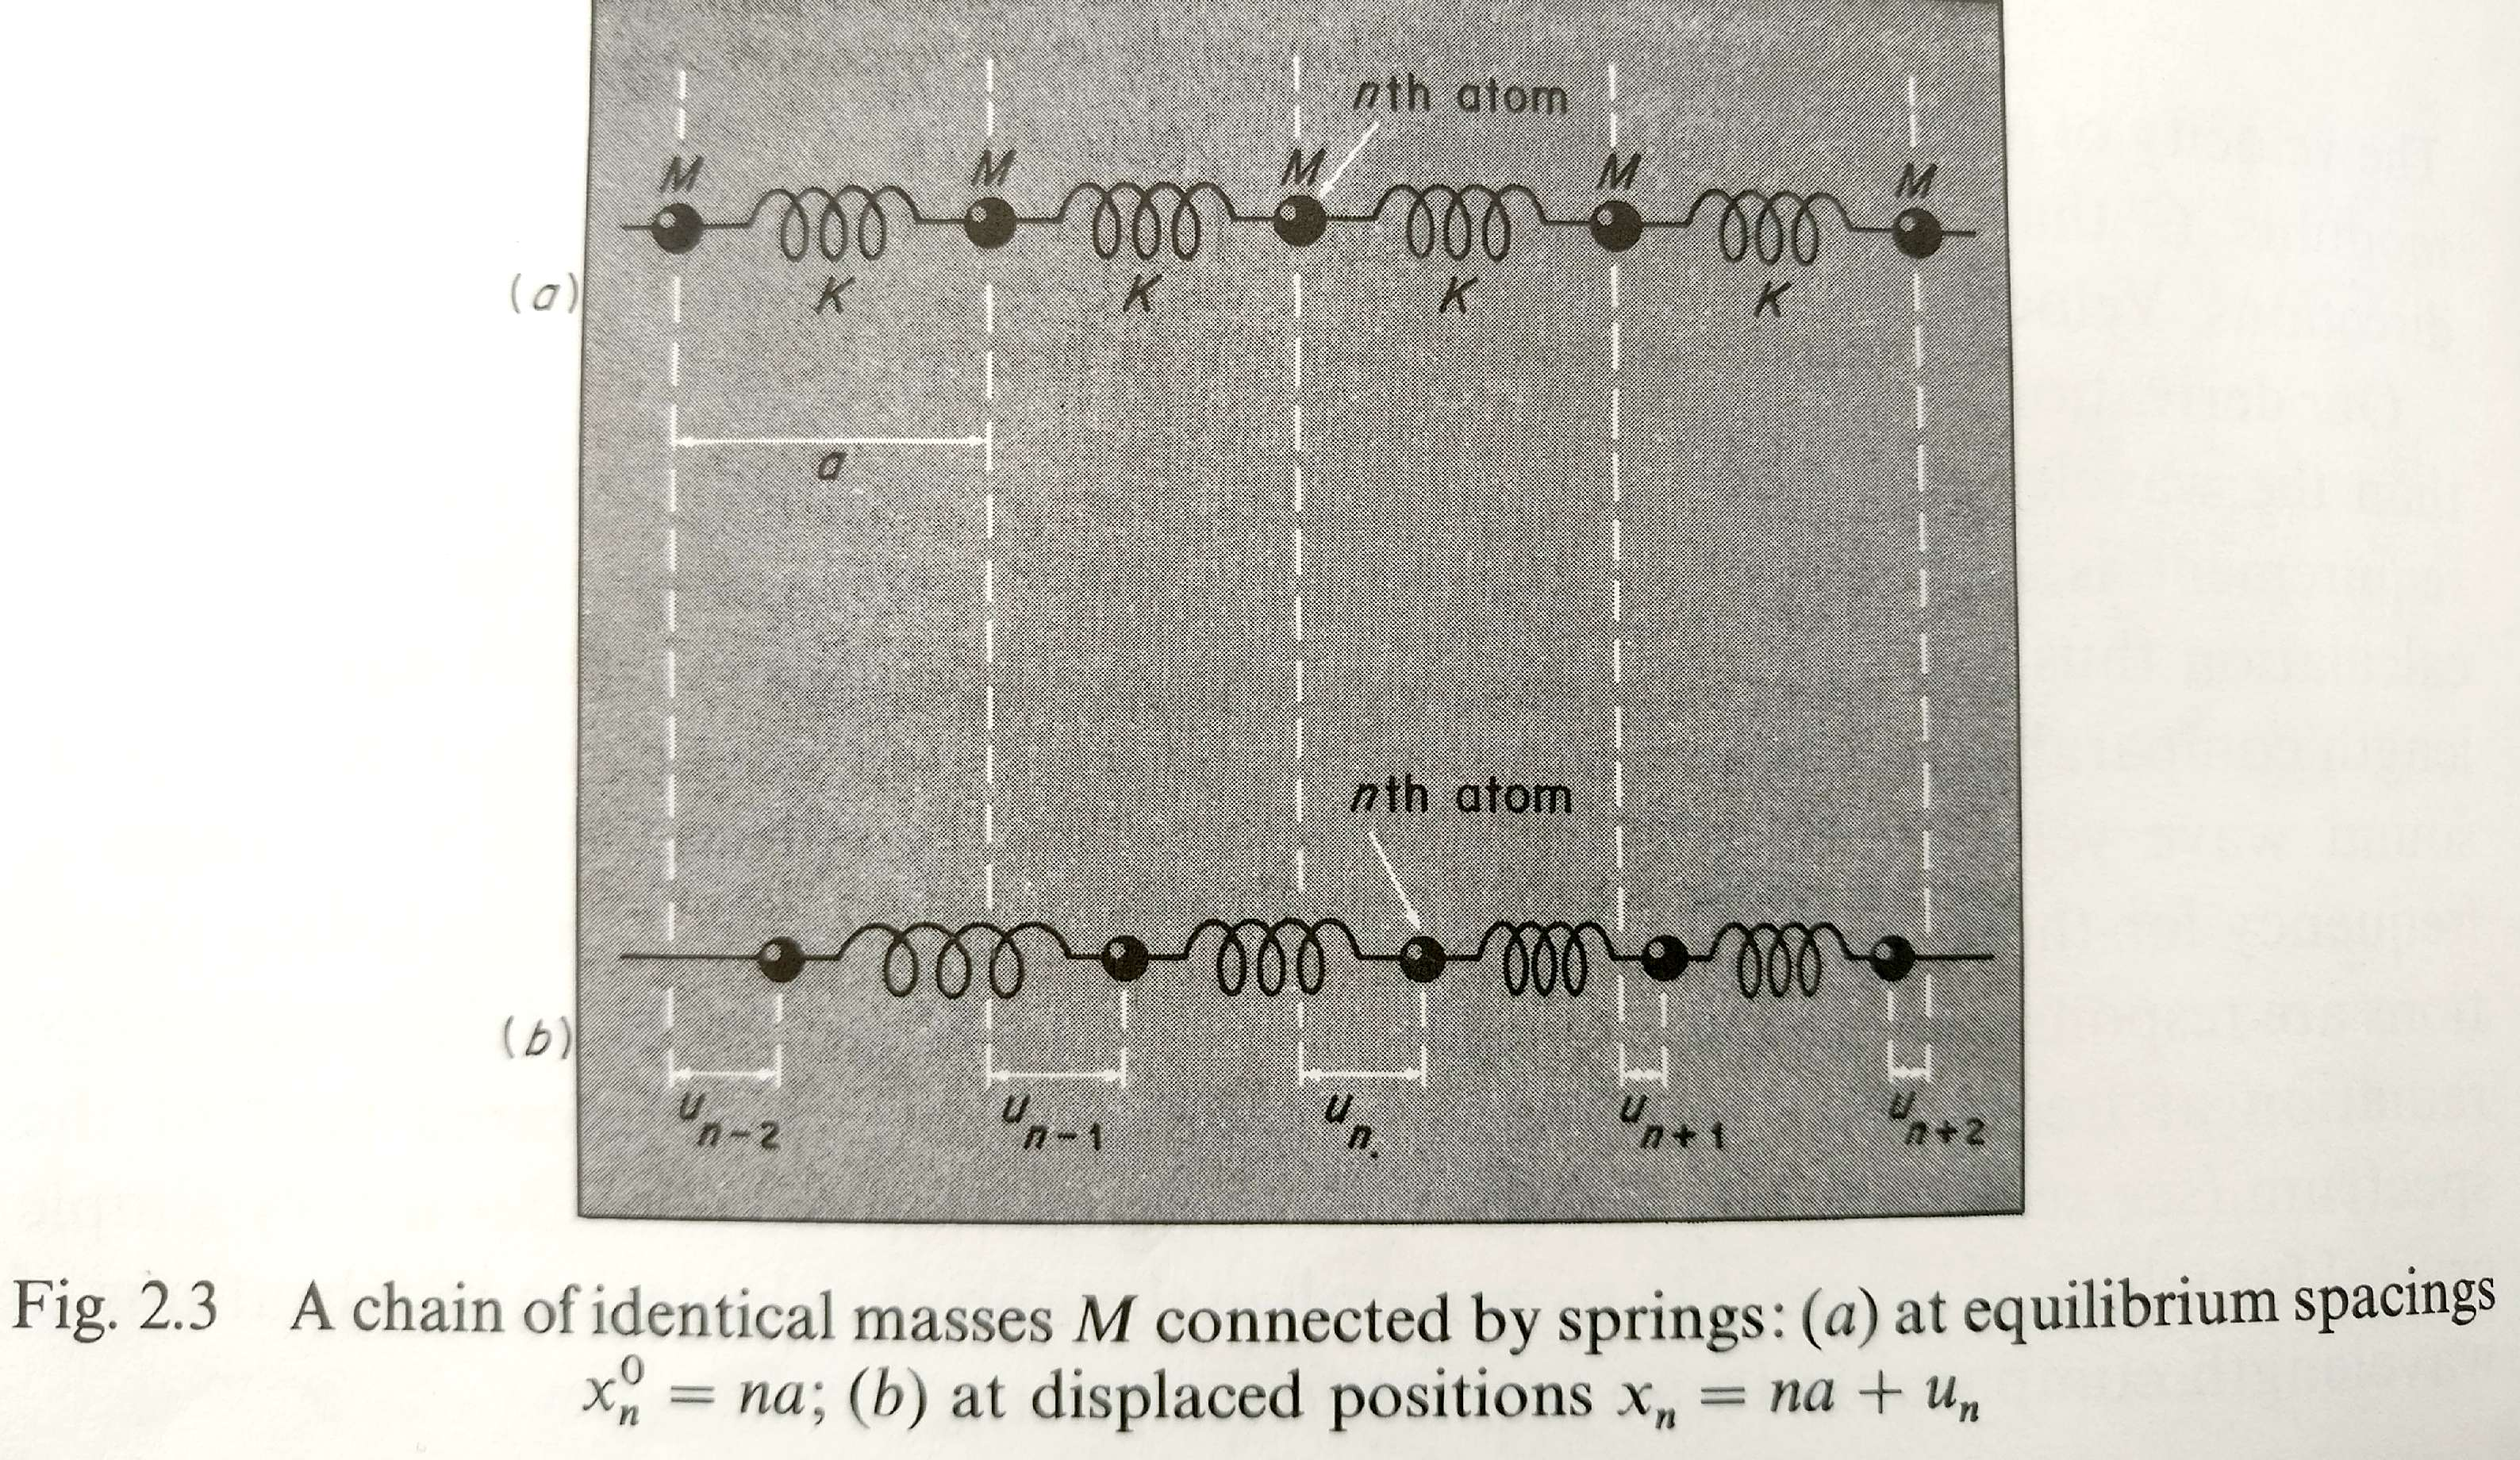
\includegraphics[width=\textwidth]{springs}
	\caption{Copied from Solid State Physics by J.R. Hook and H.E. Hall}
	\label{fig:springs}
\end{figure}

\subsection{Lattice vibrations of three-dimensional crystals}
Hand waviness about how the 1d case extends to 3d. For a unit cell containing only 1 atom three directions are possible for the wave to propagate through, so we have 3N modes. For a primitive unit cell with two atoms there are three acoustic branches and three optical branches (basically we're talking about transversal and longitudinal waves). The general result for a unit cell containing s atoms is three acoustic branches and 3(s-1) optical branches.

\subsection{Phonons}
Supposing that a lattice vibration mode of frequency $\omega$ will behave like a simple harmonic oscillator, it will thus be restricted to the energy levels
\begin{equation}
	\sigma_n = (n+\frac{1}{2}) \hslash \omega.
\end{equation}
From this we introduce the concept of a phonon, with the quanta $\hslash \omega$. We cannot determine a phonons exact position since we know the momentum $\hslash \pmb{k}$, due to the uncertainty principle. But as with photons or electrons we can create a wavepacket by combining modes of slightly different frequency and wavelength. This wavepacket represents a fairly localized phonon moving with group velocity $d\omega/d\pmb{k}$. Note now that we interpret the momentum and energy for the phonon as
\begin{align}
	E &= \hslash \omega \\
	\pmb{p} &= \hslash \pmb{k}
\end{align}
but the momentum is not the true kinematic momentum. This due to a lattice mode of wavenumber $k$ can just as well be represented by the wavenumber $k+2\pi n  /a$. Thus there is no unique value of $\pmb{k}$ ascribed to a phonon. Though we will see that this momentum we call \emph{crystal momentum} does possess many of the properties of momentum.

\subsection{Wavelike normal modes - Bloch's theorem}
In page 328-330 the book goes through how we derive the \textbf{Bloch wavefunction}. We start by assuming that the wavefunctions time dependence is $e^{i\omega t }$
\begin{equation}
	\Psi(\pmb{r},t) = \Psi(\pmb{r}) e^{i\omega t}.
\end{equation}
Then through a nice argument of incremental changes from lattice point to lattice point we end up with the expression
\begin{equation}
	\Psi(\pmb{r}_l,t) = e^{i(\pmb{k} \cdot \pmb{r}_l - \omega t)}.
\end{equation}
The derivation then does a subtle argument for going over from a more discrete space of lattices with a basis to a continuous one, this is the most difficult part to follow but we end up with
\begin{equation}
	\Psi(\pmb{r},t) = \frac{1}{\sqrt{V}} u_k(\pmb{r}) e^{i(\pmb{k} \cdot \pmb{r} - \omega t)}
	\label{eq:bloch-wavefunction}
\end{equation}
where $V$ is the volume of the crystal, and $u_k(\pmb{r})$ is a periodic function with period of the lattice, which describes the different normal modes $\pmb{k}$ which exists due to the basis associated with a lattice point. This function simply equals to unity in the case that the basis does not exists and we only have an atom on the lattice point. The term $frac{1}{\sqrt{V}}$ is just a convenient normalization factor tacked on to the expression after we normalized the function.

The very fact that that wavefunctions in a crystal can be expressed on this form is \textbf{Bloch's theorem}.
	
\subsection{Normal modes and the reciprocal lattice}
\subsubsection{periodicity of the dispersion relation}\label{sec:dispersion}
A normal mode of the crystal described by a function of the form of equation~\ref{eq:bloch-wavefunction} for some wavevector $\pmb{k}$ can also be described by function of the same form but with a different wavevector $\pmb{k}'$ related to $\pmb{k}$ by
\begin{equation}
	\pmb{k}' = \pmb{k} + \pmb{G}_0
\end{equation}
where $\pmb{G}_0$ is any vector of the reciprocal lattice of the crystal.

This is pretty cool and gives us three pretty cool effects.
\begin{enumerate}
	\item For any branch of the dispersion relation, the frequency is periodic in $\pmb{k}$-space with the same periodicity as the reciprocal lattice.
	\item Any mode can be represented by wavevector inside a single primitive unit cell of the reciprocal lattice.
	\item The number of normal modes associated with any branch of the dispersion relation is equal to the number $N_c$ of the primitive unit cells in the crystal.
\end{enumerate}
\newpage
\subsection{New words}
\begin{itemize}
	\item \textbf{Zero point motion}
	\item \textbf{Zero point energy}
	\item \textbf{Lattice vibrations}
	\item \textbf{Harmonic limit}
	\item \textbf{Crystal momentum}
	\item \textbf{Bloch wavefunction}
	\item \textbf{Bloch's theorem}
\end{itemize}
\newpage

\section{Free electrons in metals}
\subsection{Introduction}
The conductivity of electricity in solid is usually an indication that there are many electrons in the solid which is not bound to an atom, but are able to move through the whole crystal. Ignoring the fact of why this occurs we will in this section assume that all valence electrons behave in this manners for all the metals. Using the simple theory of the free electron model we will try and explain many of the properties of many metals.
\subsection{The free electron model}
We argue that the valence electrons can move freely in a metal, thus ignoring the crystal structure completely. We also ignore the repulsive interaction between conduction electrons. So we consider electrons moving independently in a square potential well of finite depth, with the edges of the well corresponding to the actual boundaries of the metal. Since the bulk properties of a piece of metal generally are independent of shape, we will consider a simple cube with sides $L$ too. What's left then is to solve the time-independent Schrödinger equation
\begin{equation}
	- \frac{\hslash^2}{2m} \nabla^2 \psi = \epsilon \psi.
\end{equation}
With periodic boundary conditions
\begin{equation}
	\psi (x+L, y+L, z+L) = \psi(x,y,z)
\end{equation}
The solution of this is
\begin{equation}
	\psi(x,y,z) = \frac{1}{\sqrt{V}} e^{i(\pmb{k}\cdot\pmb{r})}
\end{equation}
where $V = L^3$ is the volume of the metal cube, and the term involving $V$ is due to normalization. Using the boundary equation we also get
\begin{align}
	k_x = \frac{2\pi p}{L} \\
	k_y = \frac{2\pi q}{L} \\
	k_z = \frac{2\pi r}{L} 
\end{align}
and the momentum is
\begin{equation}
	\pmb{p} = \hslash\pmb{k} = \hslash(k_x, k_y,k_z)
	\label{eq:wavefunction-free-electron-gas}
\end{equation}
And the number of allowed electron states per unit energy range $g(\epsilon)$ is given by
\begin{equation}
	g(\epsilon) = \frac{V}{2\pi^2 \hslash^3} (2m)^{3/2 \sqrt{\epsilon}}
\end{equation}
where we taken into account that each electron can occupy the same energy state with a different spin.

\subsubsection{Ground state of the free electron gas}
Electrons are fermions with half-integral spin and obeys the Pauli exclusion prinicple. Thus to find the lowest energy state of $N$ free electrons we need to fill up all the lowest energies until we reach the Fermi energy $\epsilon_f$. We do this by integrating the density of states between $0$ and $\epsilon_f$.  
\begin{equation}
	N = \int_0^{\epsilon_f} g(\epsilon) d\epsilon = \frac{V}{3 \pi^2 \hslash^3} (2m\epsilon_f)^{3/2}
\end{equation}
thus we get an expression for the Fermi energy as
\begin{equation}
	\epsilon_f = \frac{\hslash^2}{2m} (\frac{3 \pi^2 N}{V})^{2/3}.
\end{equation}
We now move on to get he energy from the wavefunction for the free electron gas (equation~\ref{eq:wavefunction-free-electron-gas}) using the energy operator\footnote{$\hat{\epsilon} = i \hslash \frac{\partial}{\partial t}$}, we then get the expression
\begin{equation}
	\epsilon = \frac{\hslash^2 k^2}{2m}.
\end{equation}
From this we get the Fermi wavenumber ($k_f$) to be
\begin{equation}
	k_f = (2 \pi^2N/V)^{1/3}
\end{equation}
With this we can create the \textbf{Fermi sphere} in \textbf{k}-space as showed in figure~\ref{fig:fermi-sphere}. 
\begin{figure}[!ht]
	\centering
	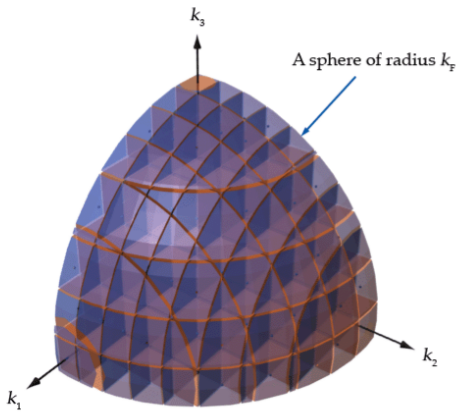
\includegraphics[width=0.5\textwidth]{fermi-sphere}
	\caption{A quarter of a Fermi sphere. The ``boxes'' represent an energy state that can be occupied. }
	\label{fig:fermi-sphere}
\end{figure}
This variables are of high importance in the following  section, together with the \textbf{Fermi momentum} ($p_f = \hslash k_f$) and the \textbf{Fermi veloctiy} ($v_f = p_f/m$). Its interesting to note that the Fermi energy would not be obtained by an electron gas due to the incredibly high temperature that is required for an electron to jump to this energy. This will however occur in a solid due to the Pauli exclusion principle, as has been showed. We also define a \textbf{Fermi temperature} through $\epsilon_f = k_b T_f$.

\subsubsection{The free electron gas at a finite temperature}
The probability that an electron will occupy a certain electron state of energy $\epsilon$ is given by the \textbf{Fermi distribution function}
\begin{equation}
	f(\epsilon,T) = \frac{1}{e^{(\epsilon - \mu)/k_B T} + 1}
\end{equation}
where $\mu$ is the chemical potential. This function is plotted in figure~\ref{fig:fermi-function}. In figure~\ref{fig:fermi-function} we also plot the number of electrons per unit energy range in thermal equilibrium, which is given through 
\begin{equation}
	n(\epsilon,T) = g(\epsilon)f(\epsilon,T).
\end{equation}
This equation becomes evident when you realize that the density of states multiplied by the probability of occupation must give this result.
\begin{figure}[!ht]
	\centering
	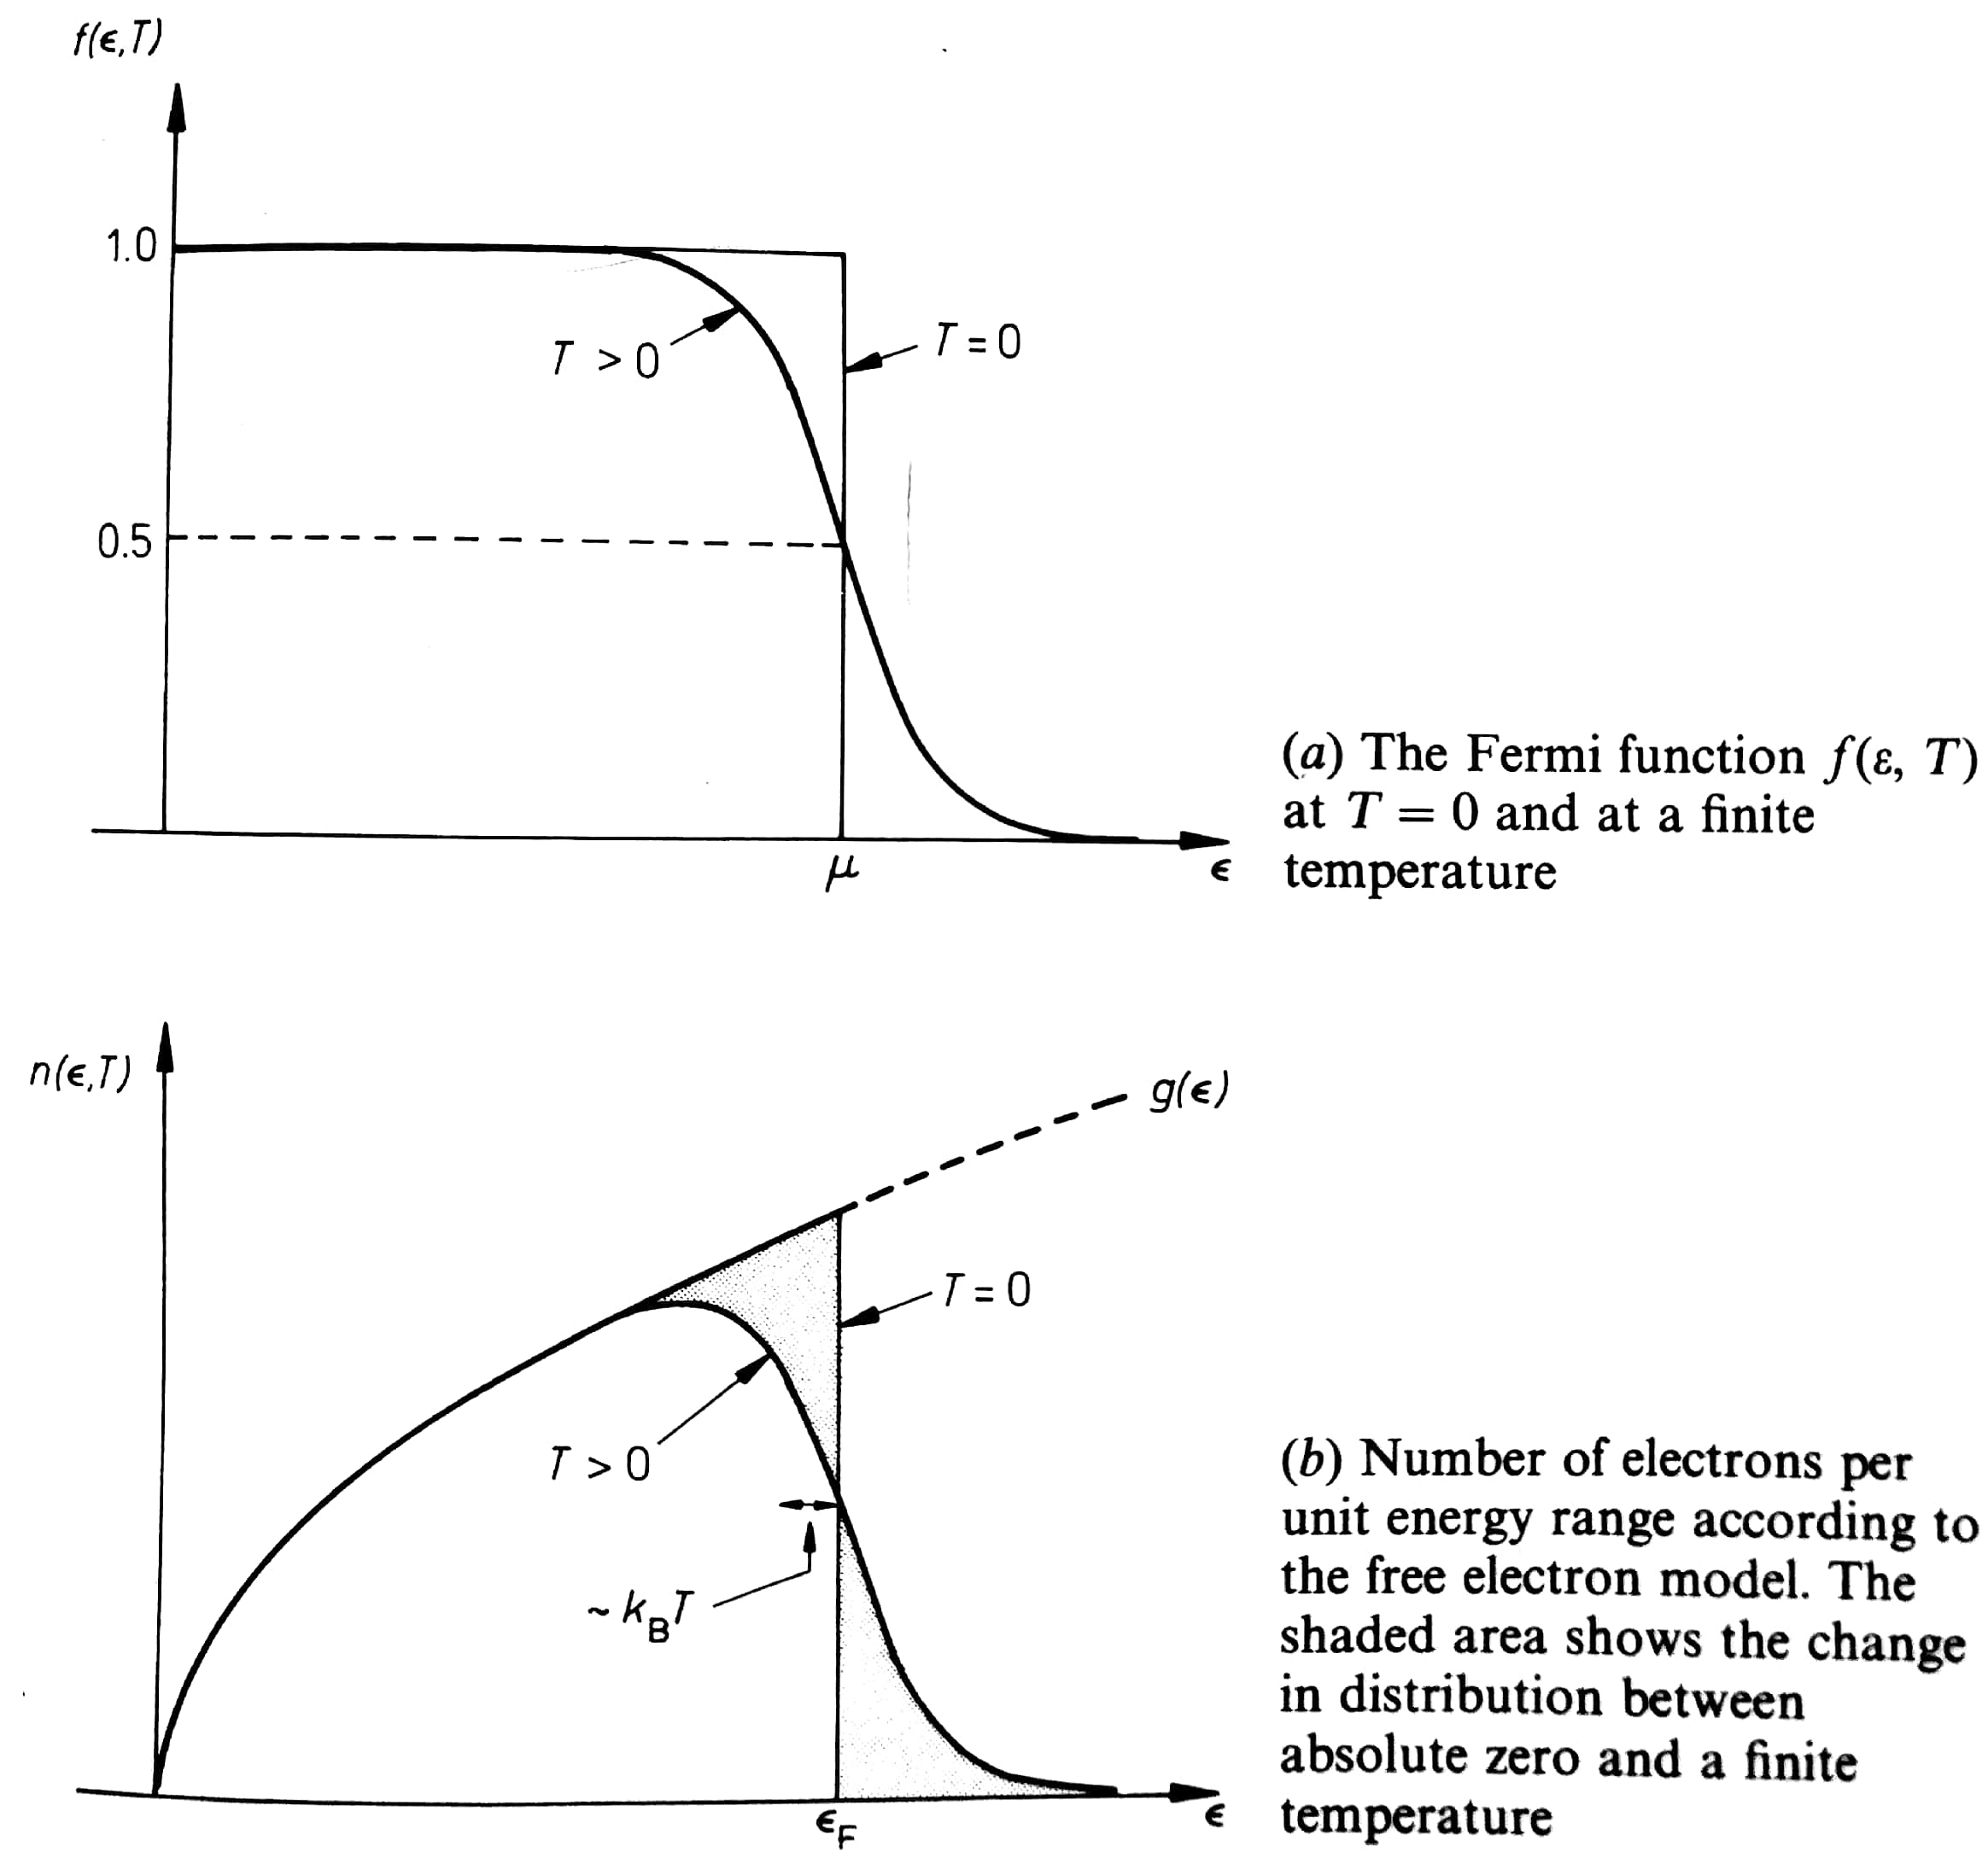
\includegraphics[width=\textwidth]{fermi-function}
	\caption{Copied from Solid State Physics by J.R. Hook and H.E. Hall}
	\label{fig:fermi-function}
\end{figure}
One can note how clear the boundaries are at $T=0$ and how it gets smoothed out around this line when the temperature is increased. It's almost like we have two triangles on each side of the clear limit when $T=0$. Given these equations we can now move on to calculate the heat capacity of the free electron gas.
\subsubsection{Heat capacity of the free electron gas}
One can start with looking at figure~\ref{fig:fermi-function} and assume the shaded areas are triangles of height $g(\epsilon)/2$ and width $2k_B T$, through this approximation we can see that the increase of energy is is equivalent to $g(\epsilon)/(2 k_B T)$ electrons having their energy increased by $k_B T$, compared to when $T=0$. We then get
\begin{equation}
	E(T) - E(0) \approx \frac{1}{2}g(\epsilon_f)(k_B T)^2.
\end{equation}
And by differentiating with respect to $T$ we get the heat capacity to be
\begin{equation}
	C_v = \frac{3}{2} N k_B (T/T_f)
\end{equation}
If we do this through exact means through carrying out the integration 
\begin{equation}
	E(T) = \int_0^\infty \epsilon n(\epsilon, T) d\epsilon
\end{equation}
and then differentiate with respect to $T$. We then get the result
\begin{equation}
	C_v = \frac{\pi^2}{2} N k_B (\frac{T}{T_f})
\end{equation}
which is pretty close, with exception to the numerical coefficient.

If we later apply this theory on the real world, we know that heat capacity in very low temperatures are described through(just given here)
\begin{equation}
	C_v = \gamma T + \beta T^3
\end{equation}
and the linear part is the one we have derived here. In potassium the difference is about 25\%, a very good result for such a simplistic view of how electrons act in metals. This discrepancy is often interpret as arising due to a difference in electrons bare mass and effective mass. But to calculate this effective mass one has to take into account the positive charge density within the crystal, i.e.\ the positively charged ions in the crystal structure. Also phonons effect the effective mass of electrons. 
\subsection{Transport properties of the conduction electrons}



\subsubsection{The equation of motion of the electrons}
Using the Lorenz force we can see that in the absence of collision we have
\begin{equation}
	m_e \frac{d\pmb{v}}{dt} = - e\pmb{E} - e\pmb{v} \times \pmb{B}
	\label{eq:force-electron}
\end{equation}
as the equation of motion for electrons. $m_e$ in this case is the effective mass, something that enables us to compensate later.

In order for this equation to hold for a wavepacket-electron\footnote{Lorentz force is a force that should act on a classical particle, not a wavefunction} we must create a somewhat localized wavepacket, with reasonably well defined position and momentum. In order to get a wavepacket localized in position to about 10 atomic spacings require use of a wavenumber range in the order of $\frac{k_f}{10}$\footnote{$k_f$ is the of the order of an inverse atomic spacing}. We also need need the packet to be smaller then then length scale associated with variation of $\pmb{E}$ and $\pmb{B}$ as well as the mean free path between collisions of electrons. But the wavepacket also have to be that the packet must be much larger then the atomic spacing in order to be able to ignore the electron-ion interaction. For such a wavepacket we have
\begin{equation}
	\pmb{v} = \frac{d\omega}{d \pmb{k}} = \frac{1}{\hslash} \frac{d \epsilon}{d \pmb{k}} = \frac{\hslash \pmb{k}}{m_e} = \frac{\pmb{p}}{m_e}
\end{equation}
which produces the expected result for a classical particle.

In equation~\ref{eq:force-electron} we have not taken inte account the effect of electron collisions in the crystal structure due to thermal vibrations in the ion cores, or due to impurities in the crystal. If this was not the case the electrons with accelerate infinitely with an applied electrical field. Thus we modify equation~\ref{eq:force-electron} in order to take into account for this
\begin{equation}
	m_e (\frac{d\pmb{v}}{dt} + \frac{\pmb{v}}{\tau} )= - e\pmb{E} - e\pmb{v} \times \pmb{B}
	\label{eq:force-electron-decay}
\end{equation}
this additional term basically creates a exponential decay to zero with a time constant $\tau$ as one remove the field upon the electrons.

\subsubsection{The electrical conductivity}
Imagine we only a DC-field, then equtaion~\ref{eq:force-electron-decay} has the steady state solution
\begin{equation}
	\pmb{v} = -\frac{e\tau}{m_e}\pmb{E}
\end{equation}
Hence the electric current density is 
\begin{equation}
	\pmb{j} = n(-e)\pmb{v} = \frac{ne^2\tau}{m_e} \pmb{E} = \sigma \pmb{E}
\end{equation}
where $\sigma$ is the electrical current, and where
\begin{equation}
	\sigma = \frac{n^2\tau}{m_e} = ne\mu_e
	\label{eq:sigma}
\end{equation}
where $\mu_e$ is the mobility of the electrons, defined as
\begin{equation}
	\mu_e = \frac{e\tau}{m_e}
\end{equation}

Through experiments one have found that there is two effects that effects the collision time of electrons. The first one is temperature, with an increased temperature the crystal structure vibrates and tend to collide more with moving electrons. The other is impurities. Impurities seem to create a constant decrease of collision time, no matter the temperature. Thus we rewrite $\frac{1}{\tau}$ as
\begin{equation}
	\frac{1}{\tau} = \frac{1}{\tau_{pu}(T)} + \frac{1}{\tau_0}
\end{equation}
where $\tau_ph$ is due to thermal vibration in the crystal structure, and $\tau_0$ is due to impurities. Using this equation one can rewrite the resistivity of metals $\rho = \frac{1}{\sigma}$ as
\begin{equation}
	\rho = \rho_l(T) + \rho_0
\end{equation}
where $rho_l$ is due to lattice vibrations, and $\rho_0$ is due to impurities. An exercise of plugging numbers will show that the length scale of collisions are much longer then interatomic spacing, which means that the electrons don't collide with the atoms themself, but actually the phonons created by the lattice vibrations\footnote{This is showed in page 89 of the book}.

\subsubsection{The thermal conductivity}
Basically thermal conductivity in metals are dominated by electrons, one can even induce currents in metals by creating a heat gradient in a metal. Using the elementary kinetic theory for thermal conductivity one gets the expression for the the thermal conductivity to be
\begin{equation}
K = \frac{\pi^2 nk_B^2 T \tau}{3m_e}{3m_e}
\label{eq:thermal-conductivity}
\end{equation}

\subsubsection{The Wiedmann-Franz law and the temperature dependence of the electrical and thermal conductivities}
If we look at equation~\ref{eq:thermal-conductivity} for the thermal conductivity and~\ref{eq:sigma} for the electrical resistance, we notice they both contain the same electron gas parameters. Dividing this should give a constant, something known as \textbf{Wiedemann-Franz law}. But it doesn't, why? The answer lies in the fact that we assumed that the collisions times that occurs due to thermal effects are the same as electrical effects. This does not hold, and a nice argument is made for this in the book on pages 90-91. As a reminder we can look at figure~\ref{fig:fermi-change}, the first image is equilibrium, while the second shows typical effects due to current relaxation, while the last image shows how heat relaxes differently, mostly due to the more average effect of the electron states, heat mostly effects states close to the Fermi sphere boundary. This displacement of k states on the x-axis corresponds to an electron velocity in the x-direction. Why the difference exists between thermal and electrical collisions time is due to how phonons and electrons interact, which is described in pages 95-96 in the book, in a kind of hand waviness manner. 
\begin{figure}[!ht]
	\centering
	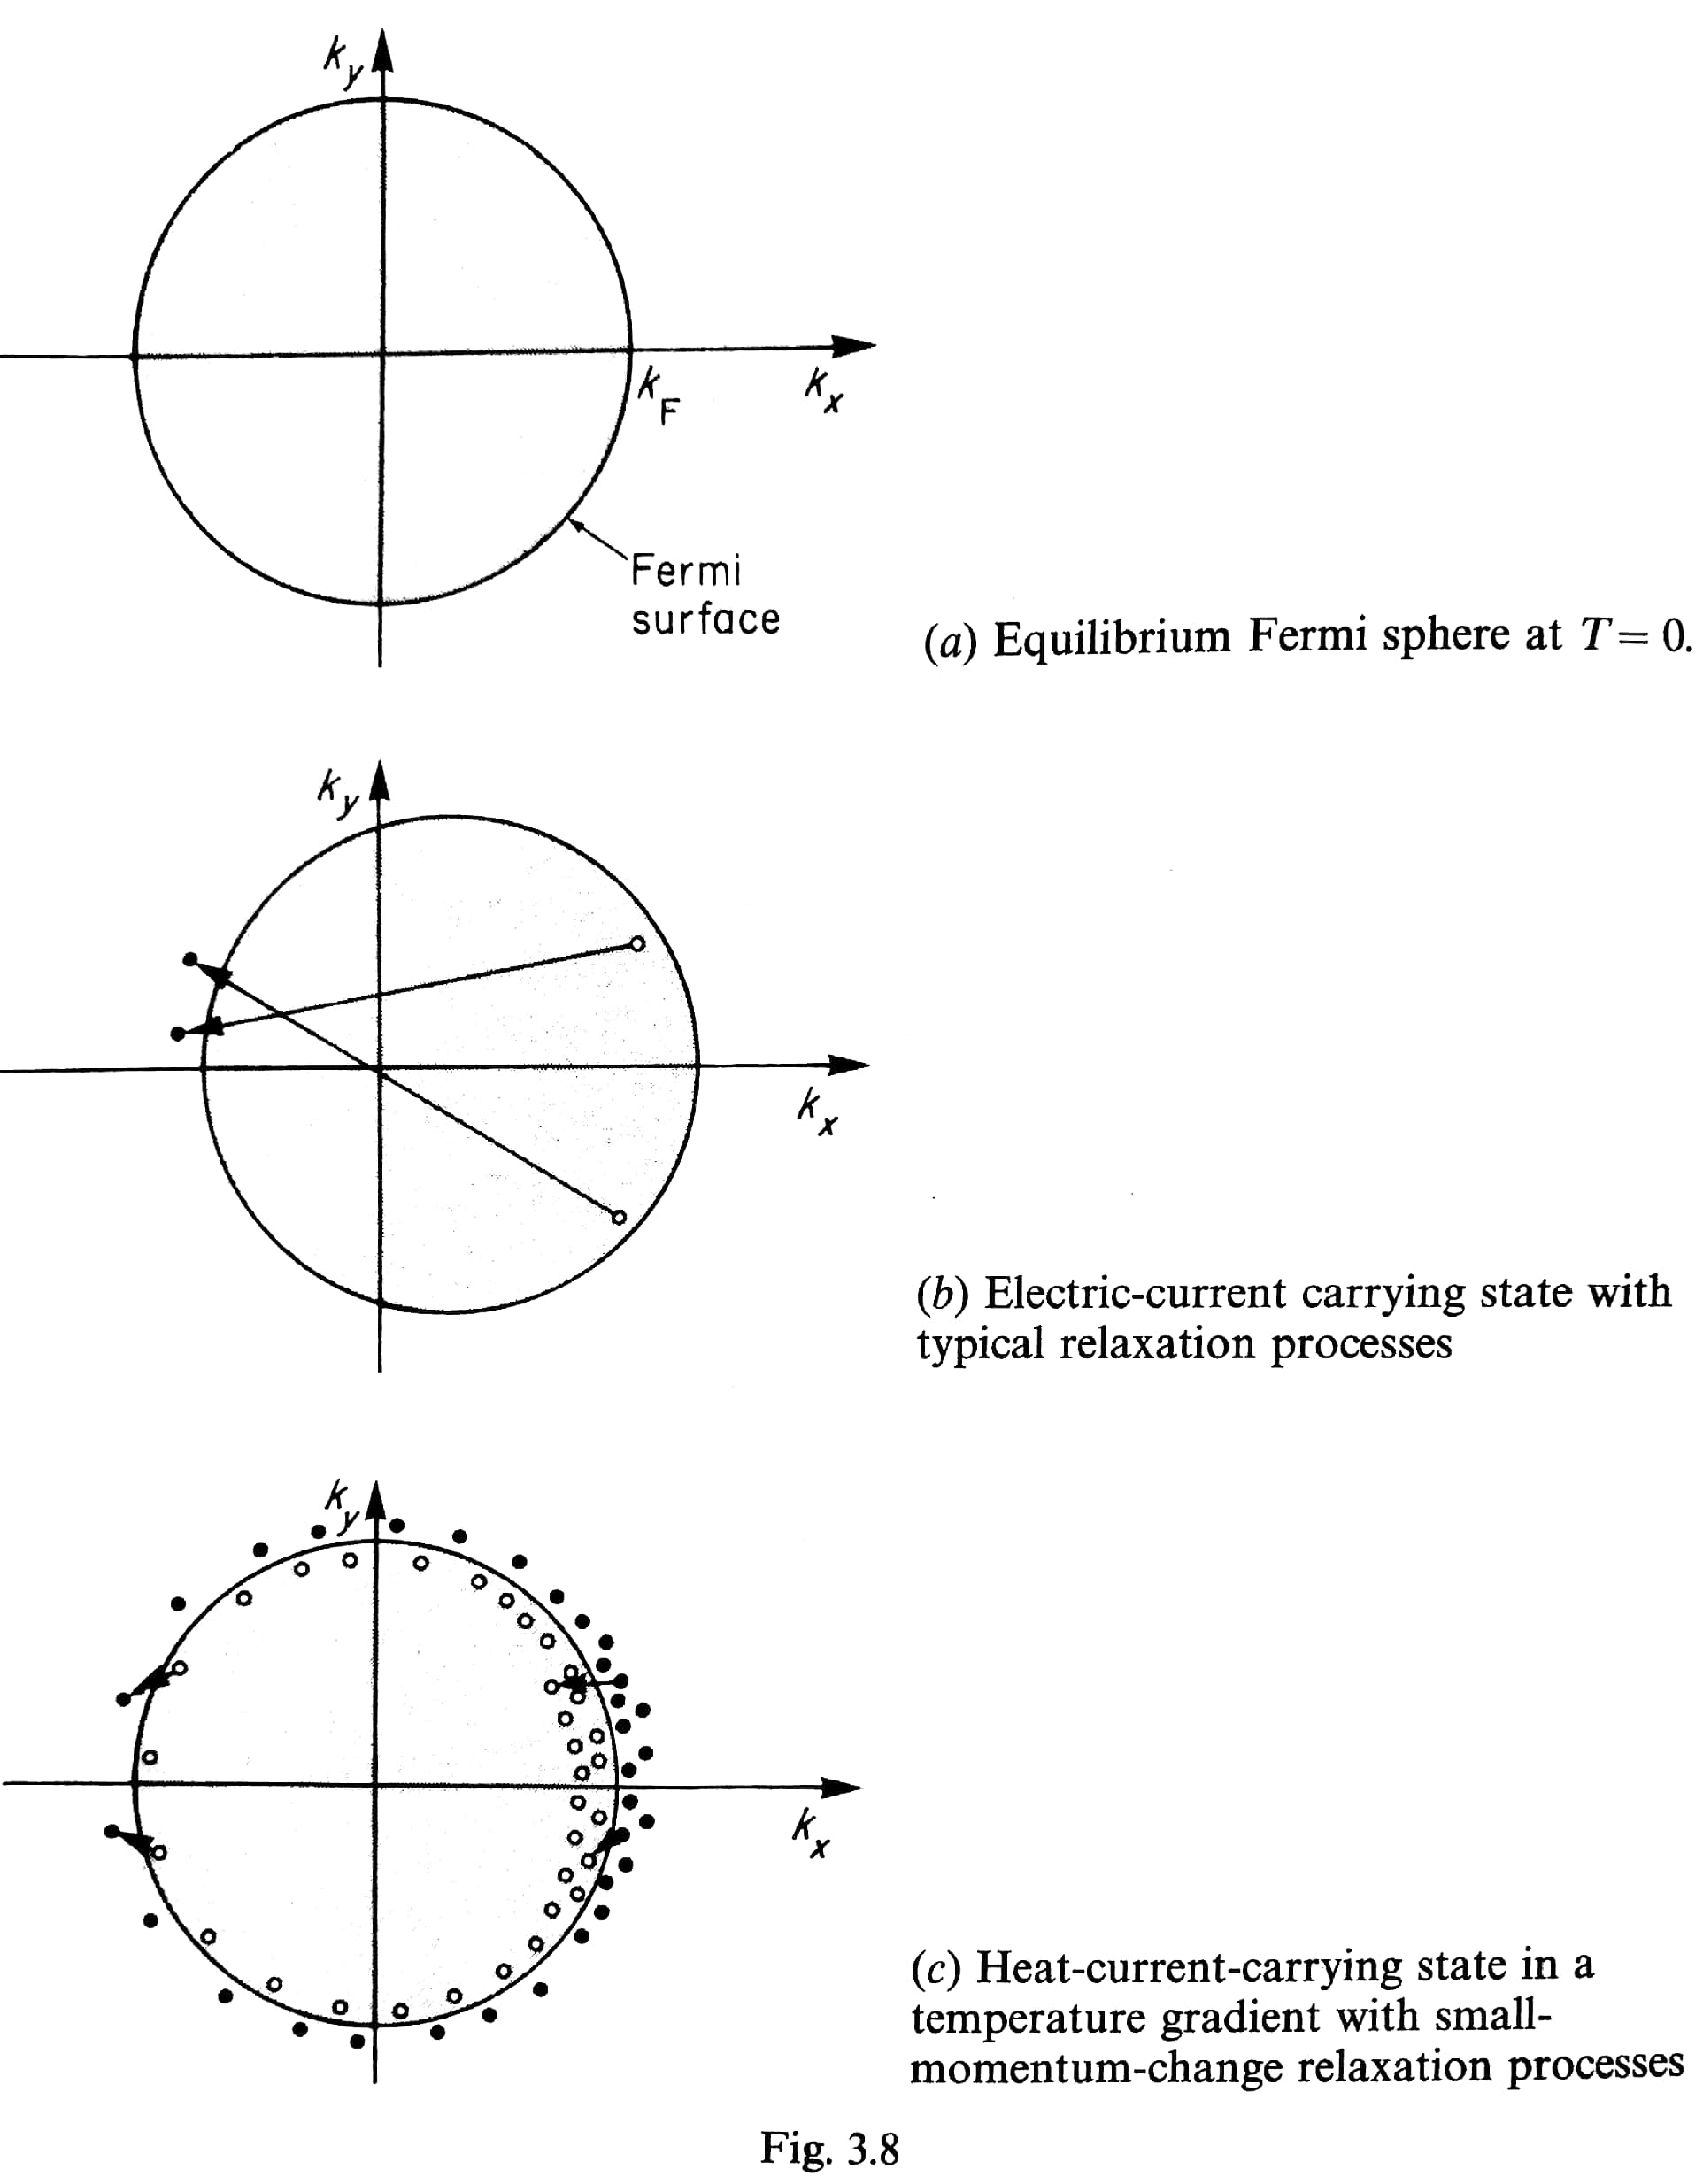
\includegraphics[width=0.7\textwidth]{fermi-change}
	\caption{Copied from Solid State Physics by J.R. Hook and H.E. Hall}
	\label{fig:fermi-change}
\end{figure}

\subsubsection{The Hall effect}
The free electron model is not very good for explaining the hall effect, for fucks sake\ldots We don't even get the same sign for some metals. 
\section{The effect of the periodic lattice potential - energy bands}
\subsection{Nearly free electron theory}

The free electron model is shit, let us use a periodic potential instead! We do it by estimating a correction to the free electron energy by using the standard formula of first-order perturbation theory
\begin{equation}
\Delta \epsilon = \frac{\int \psi^* V \psi dx}{\int \psi^* \psi dx}
\end{equation}
Where $V$ is the difference between the true potential and the constant potential assumed in the calculations for the free electron model, and $\psi$ is the unperturbed wavefunction. We also assume that the potential from the lattice is quite weak.

If we take the free electron potential to be the mean value of the true potential, then the perturbation $V$ for our one-dimensional example can be written as Fourier series in the form 
\begin{equation}
	V = - \sum^\infty_{n=1} V_n \cos{(\frac{2\pi n x}{a})}
\end{equation}
	where $V_n$ is expected to be positive for a potential with strong negative peaks at the lattice sites. Putting things together we end up with an expression that only evaluates to a value if $k=n\pi/a$. So
\begin{equation}
	\Delta \epsilon = \frac{\int dx V_n \cos^2(2\pi n x/a)}{\int dx} = \frac{1}{2} V_n
\end{equation}
if $\psi = sin(kx)$, for $\psi = cos(kx)$\footnote{Author need to brush up on quantum mechanics} we get
\begin{equation}
	\Delta \epsilon = - \frac{1}{2} V_n
\end{equation}
If one does some more proper evaluation, one finds that the energy is as depicted versus the free electron energy $\epsilon(k)$ as in figure~\ref{fig:energy-band}. Here we see \textbf{Energy bands} and \textbf{Energy gaps}.
\begin{figure}[!ht]
	\centering
	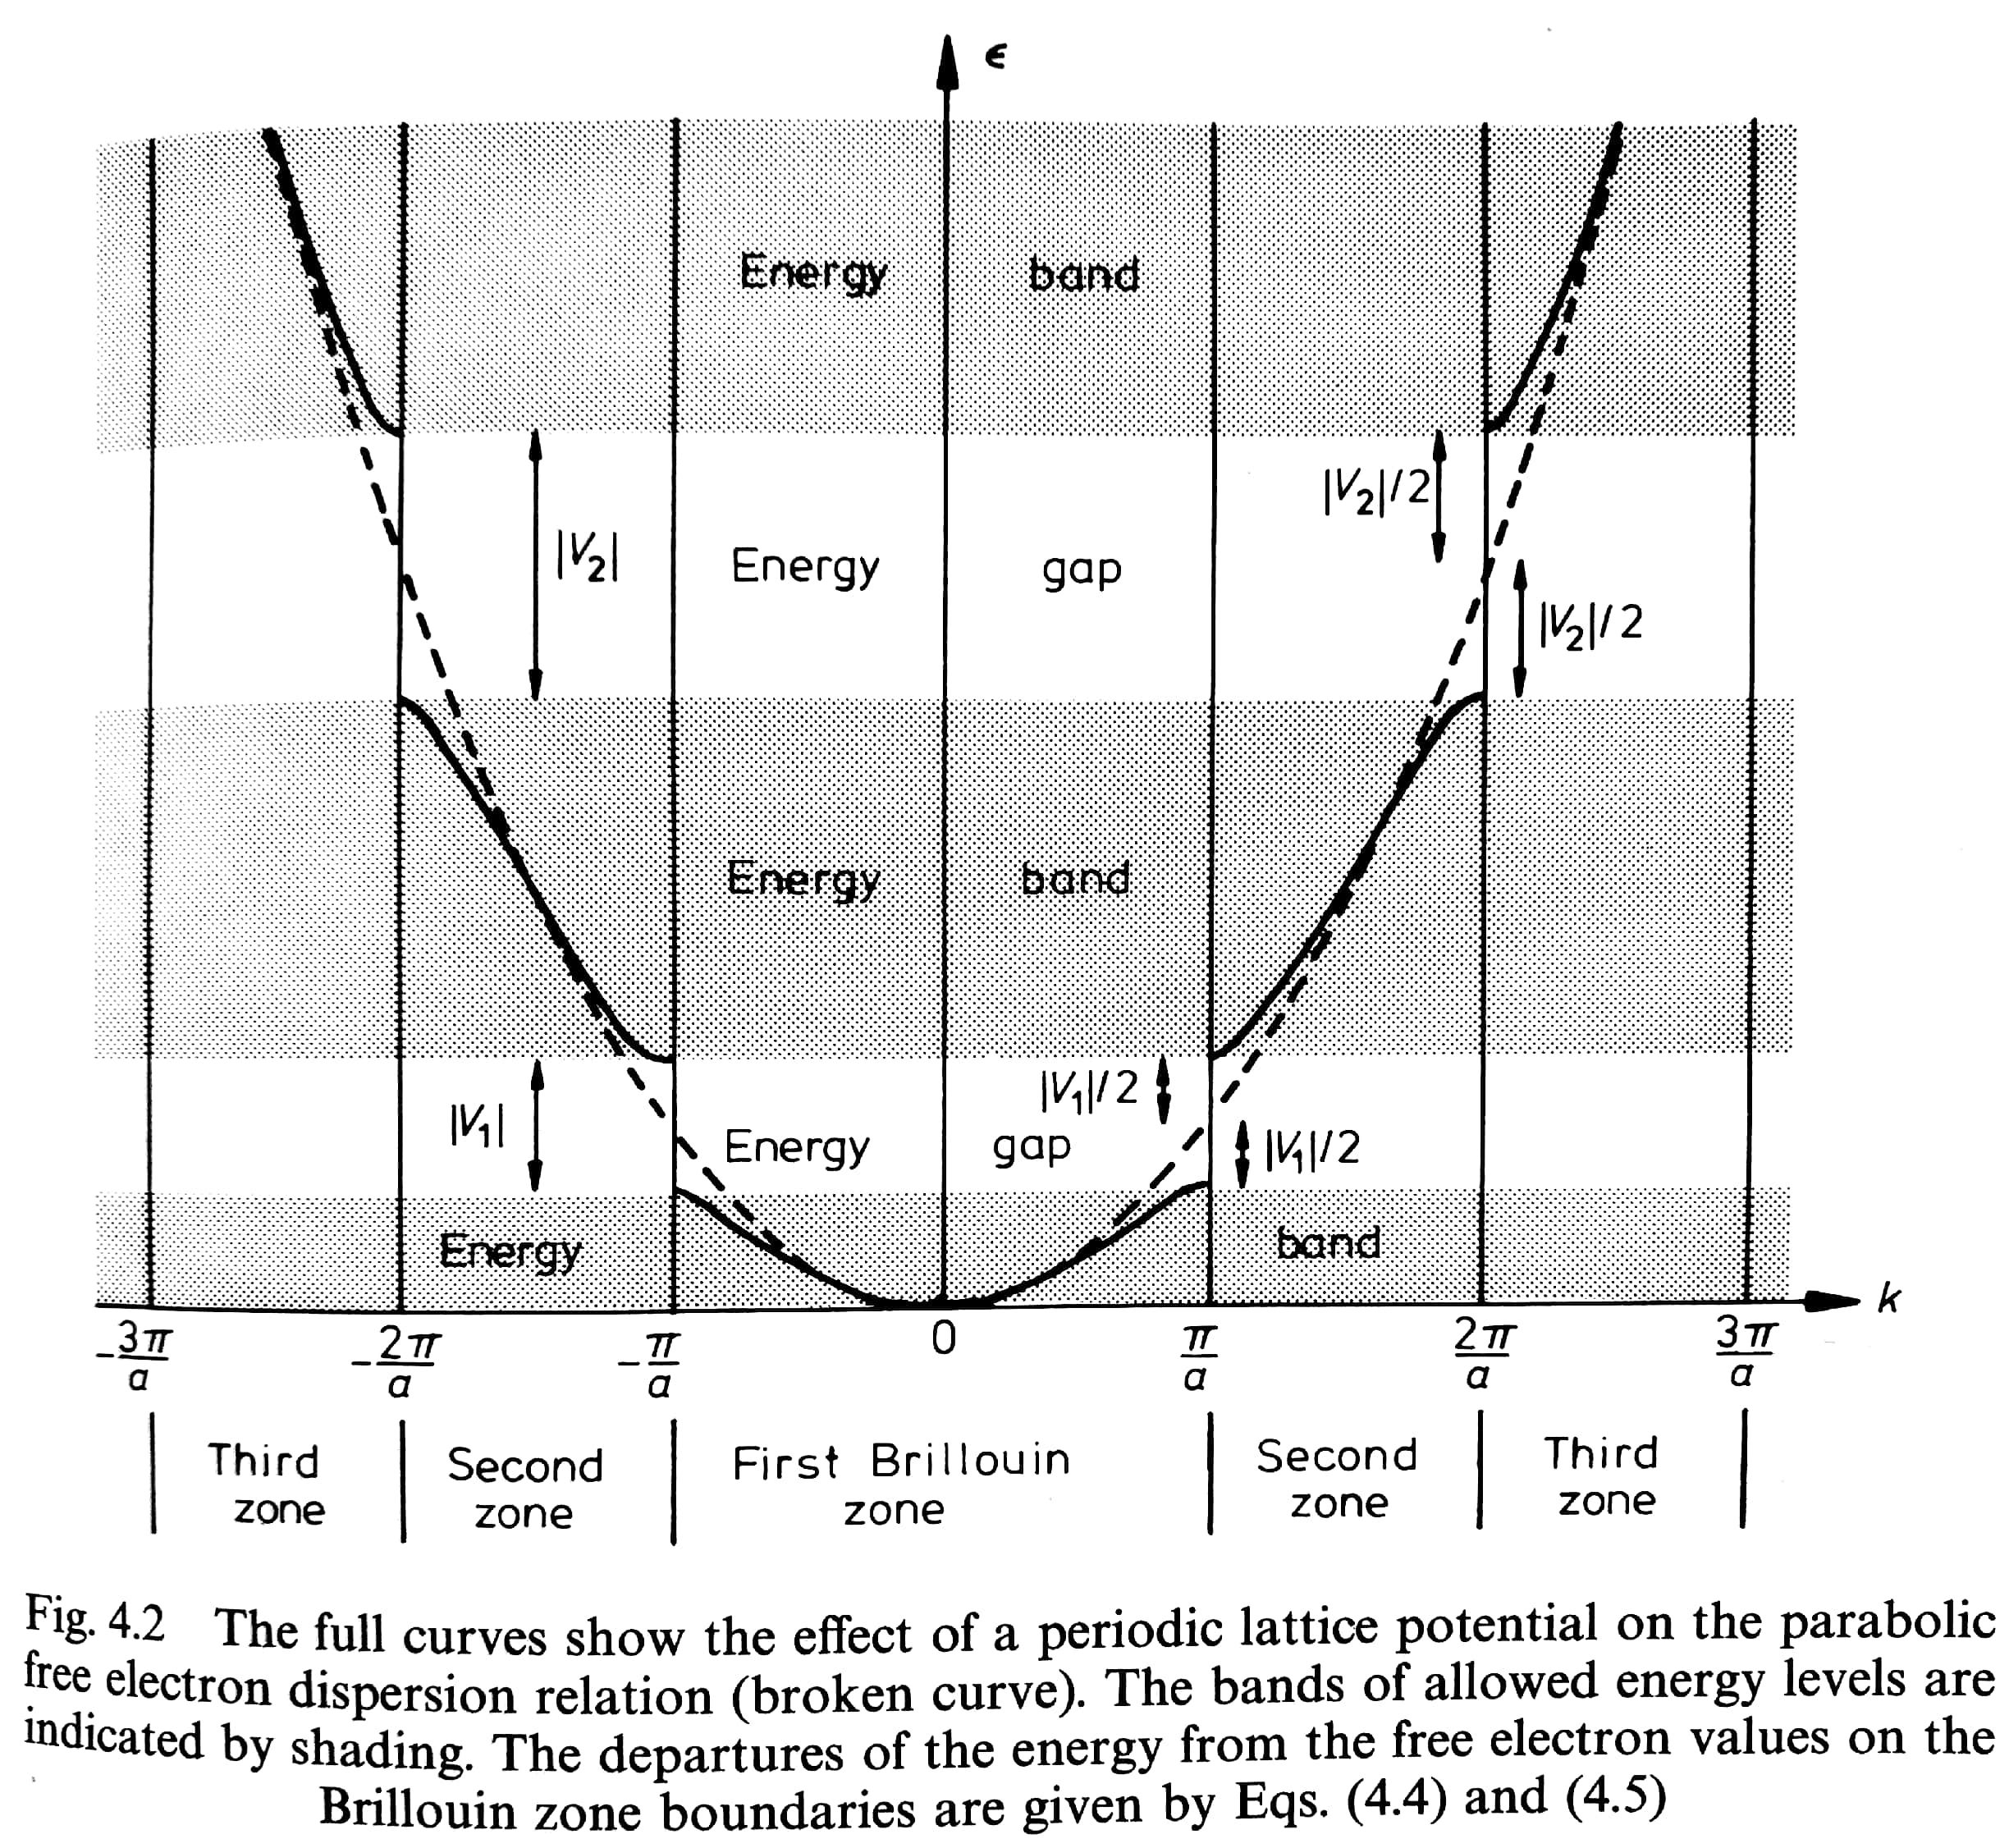
\includegraphics[width=0.7\textwidth]{energy-band}
	\caption{Copied from Solid State Physics by J.R. Hook and H.E. Hall}
	\label{fig:energy-band}
\end{figure}
We can see that the $k$ axis in figure~\ref{fig:energy-band} also are divided into region, called \textbf{Brillouin zones}, where the first Brillouin zone correspond to the lowest energy and so on.

\subsection{Classification of crystalline solids into metals, insulators and semiconductors}
We have so far only looked at the one dimensional case. We will continue to do so here but try and explain why some materials are metals, and conduct electricity, while some are insulators. If we look at the $\epsilon(k)$ relation in figure~\ref{fig:energy-band} we can see that in the first band we have every state contained in the $k$ range $(-\frac{\pi}{a},\frac{\pi}{a})$. This is further zoomed in to in figure~\ref{fig:energy-jump}. We know that $k = 2 \pi p /L$, $L = Na$, and that electrons are fermions with half spin, thus two electrons are able to share the same energy state. Thus we have in the first band space for $2N$ electrons. So if we have monovalent\footnote{One valence electron} atom structure, then we have the situation as depicted in picture $(a)$ of figure~\ref{fig:energy-jump}. So if we add current to the solid, the Fermi space will be moved in the direction, and there is a almost continuous amount of states in each direction of the k-space. This make it very easy to conduct electricity through, we have a metal! On the other hand\ldots if we have 2 valence electrons in the atom then we have the situation depicted in picture $(b)$ of figure~\ref{fig:energy-jump}. Here all 2N states of the first band is taken in an unperturbed state, i.e.\ when we have no current through it. So in order to move a current through it we need so much energy so the electrons can be excited to the next energy band. Thus we have an insulator!
\begin{figure}[!ht]
	\centering
	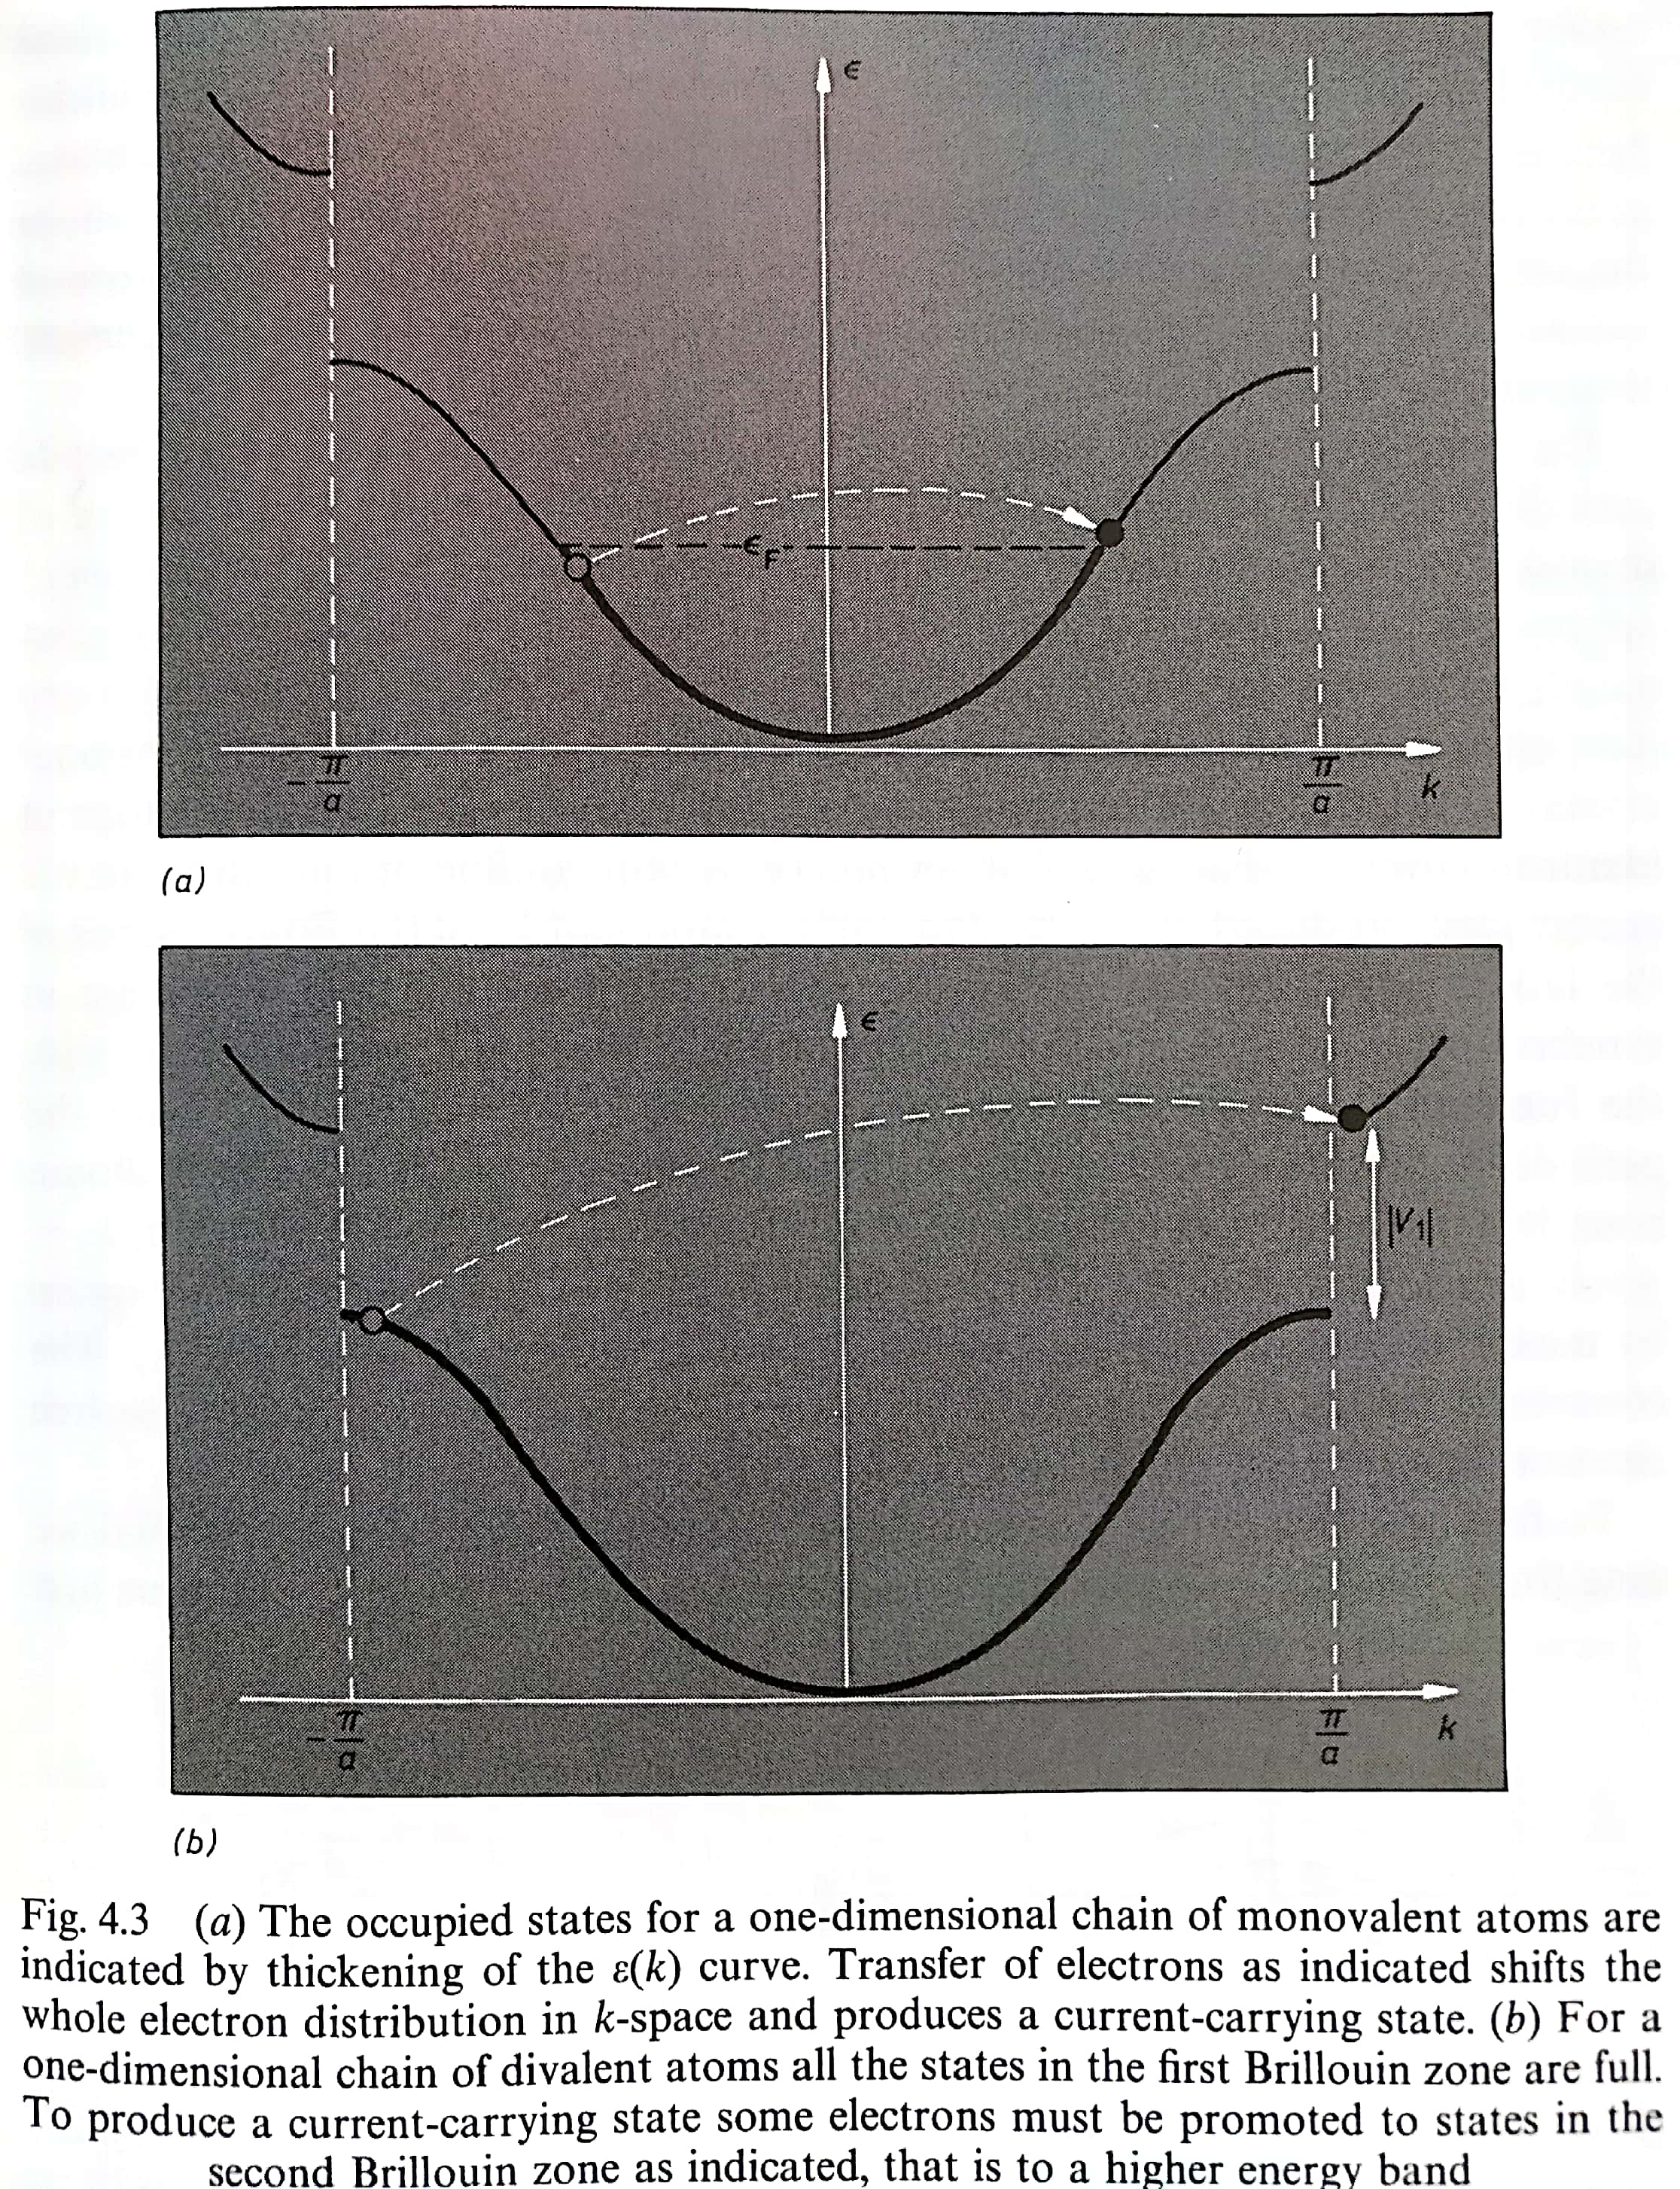
\includegraphics[width=0.7\textwidth]{energy-jump}
	\caption{Copied from Solid State Physics by J.R. Hook and H.E. Hall}
	\label{fig:energy-jump}
\end{figure}

Problem with this picture in one dimension is that we actually have metals with two valence electrons. But this is solved if we look into a two dimensional structures, cause then we can get overlapping bands in some situations. First we should mention that the energy gap size is directly correlated to the potential strength, so we have larger energy gaps with a higher periodic potential, and smaller with a smaller potential. A smaller potential then is the requirement in order to get overlapping band. That said no matter how low this potential is we still get gaps in the one dimensional case. If we look at figure~\ref{fig:2d-fermi} we can see how we could construct the free electron gas in a simple two dimensional square crystal. In the book we only make a hand waviness argument for saying that with a potential the first energy band should look like figure~\ref{fig:2d-fermi-perturbated}. This argument is made around how the difference looked like in the one dimensional case and then graphically translate it to  two dimension. 
\begin{figure}[!ht]
	\centering
	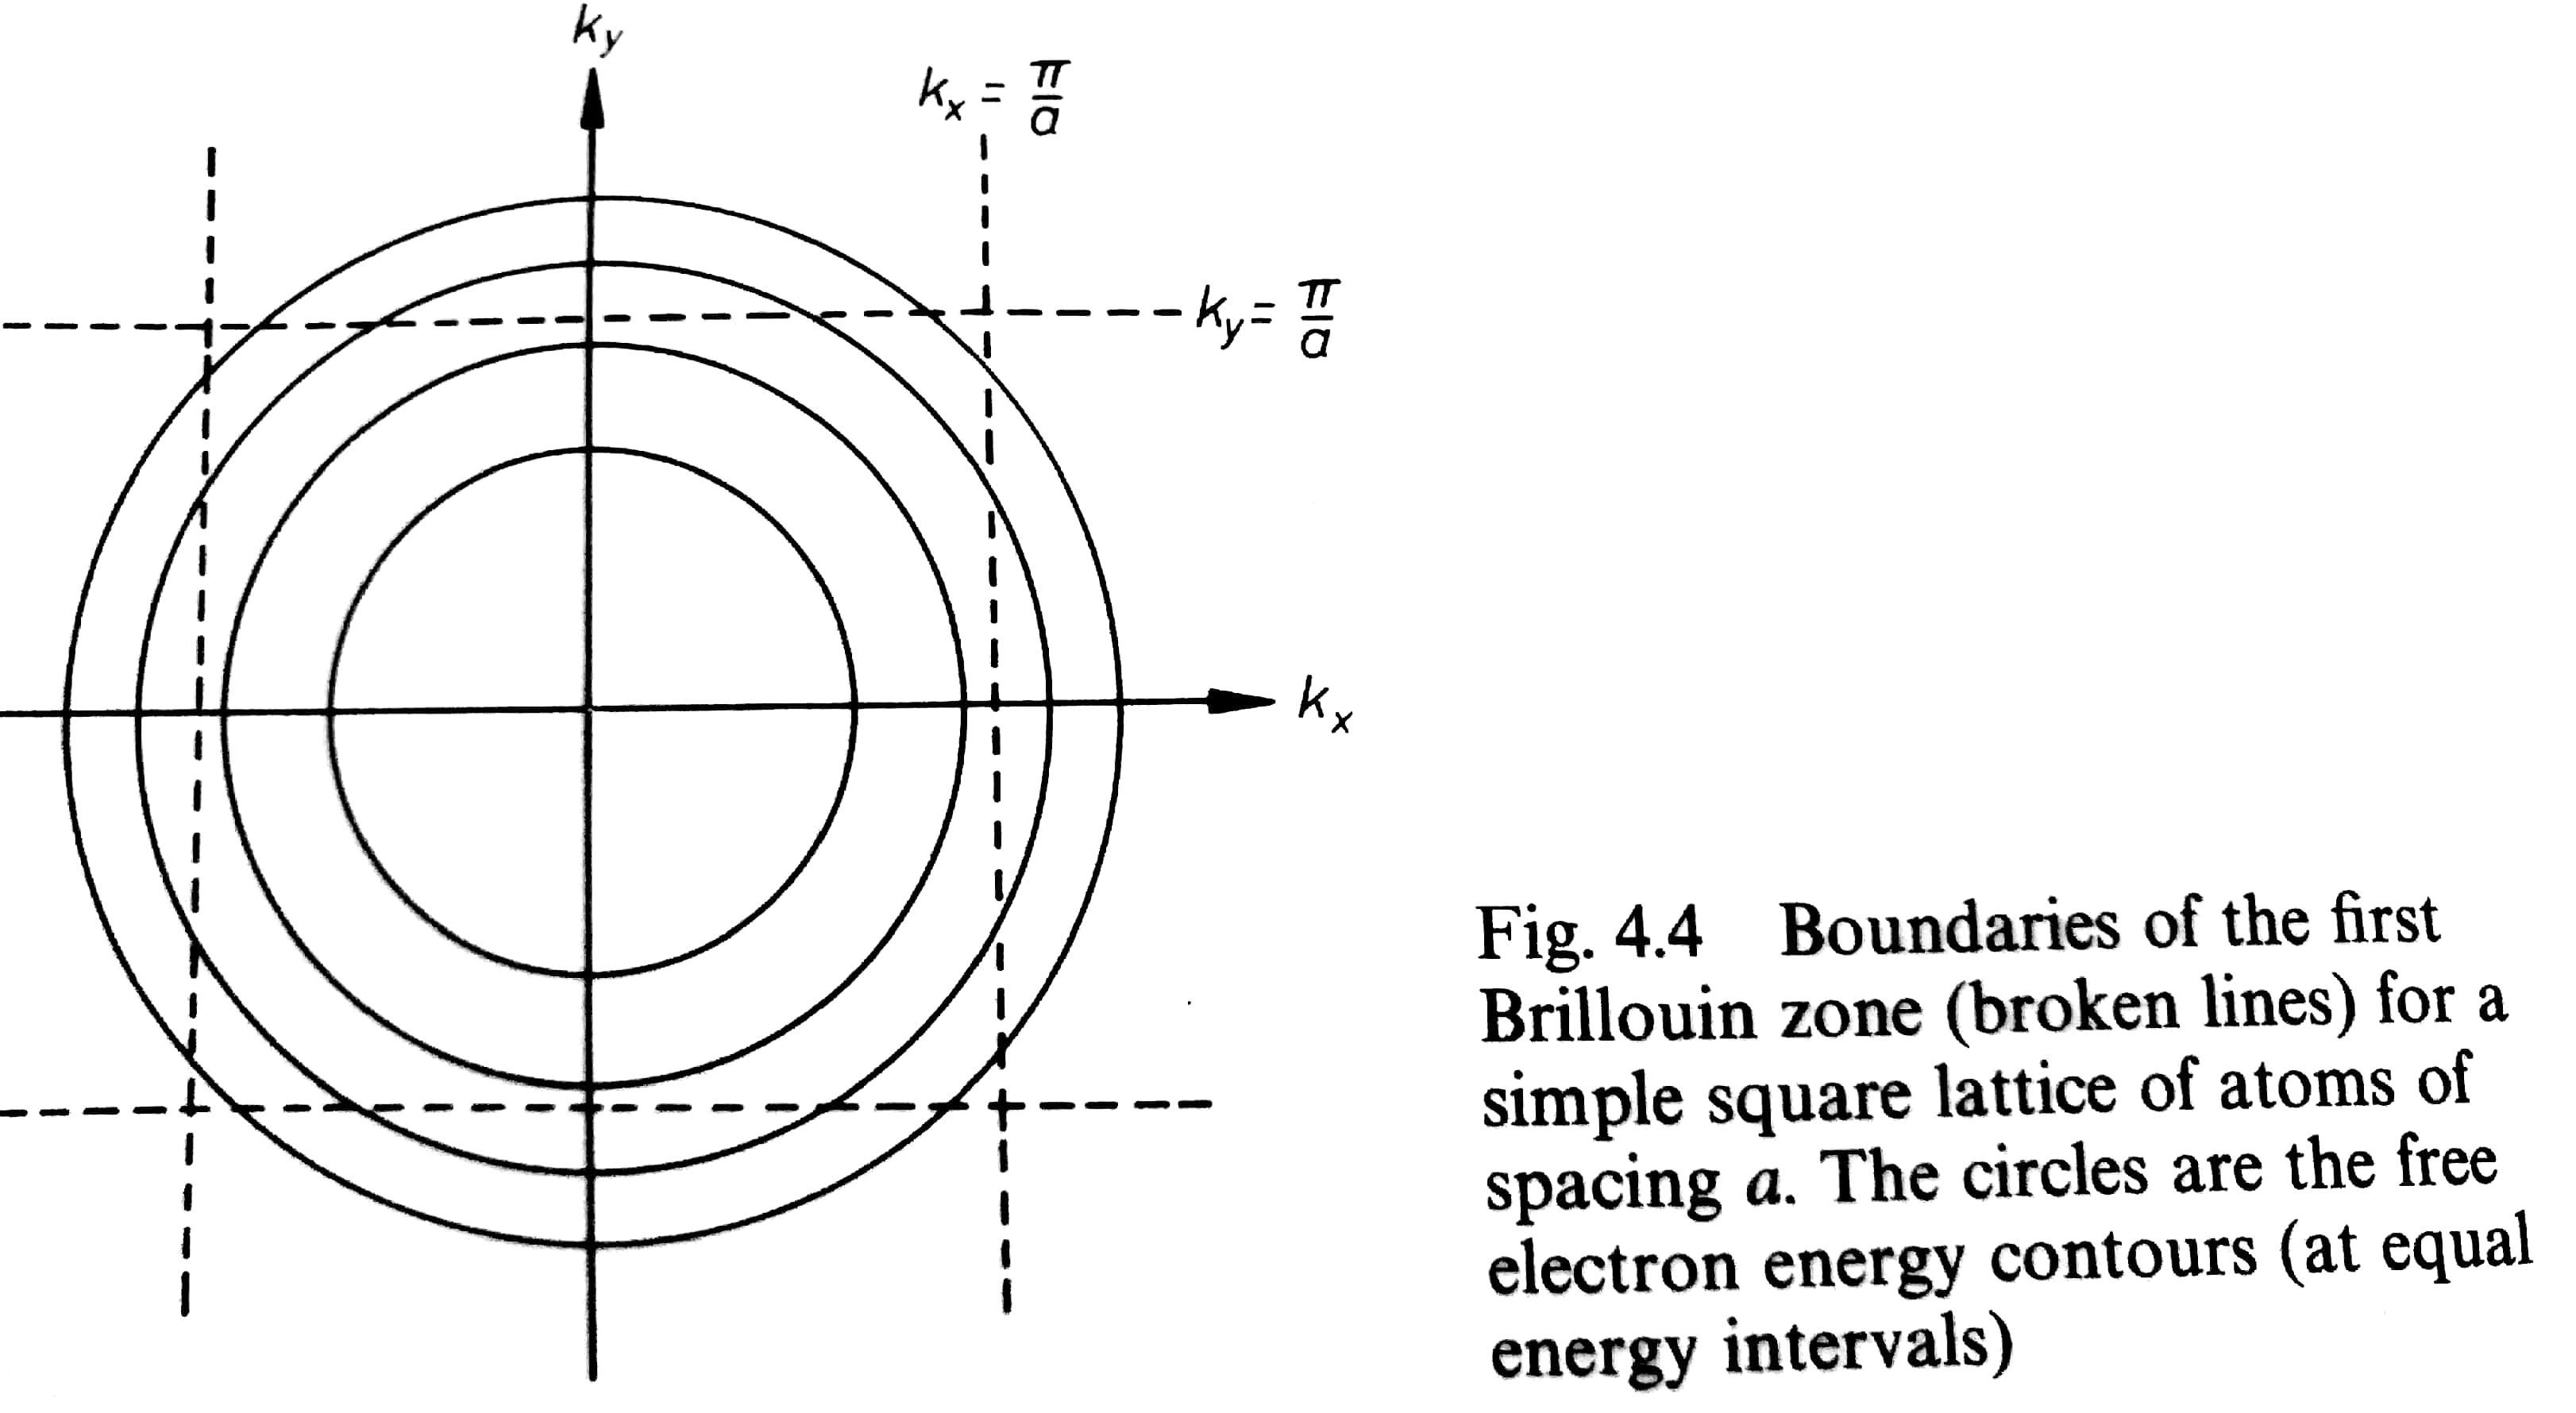
\includegraphics[width=0.7\textwidth]{2d-fermi}
	\caption{Copied from Solid State Physics by J.R. Hook and H.E. Hall}
	\label{fig:2d-fermi}
\end{figure}
\begin{figure}[!ht]
	\centering
	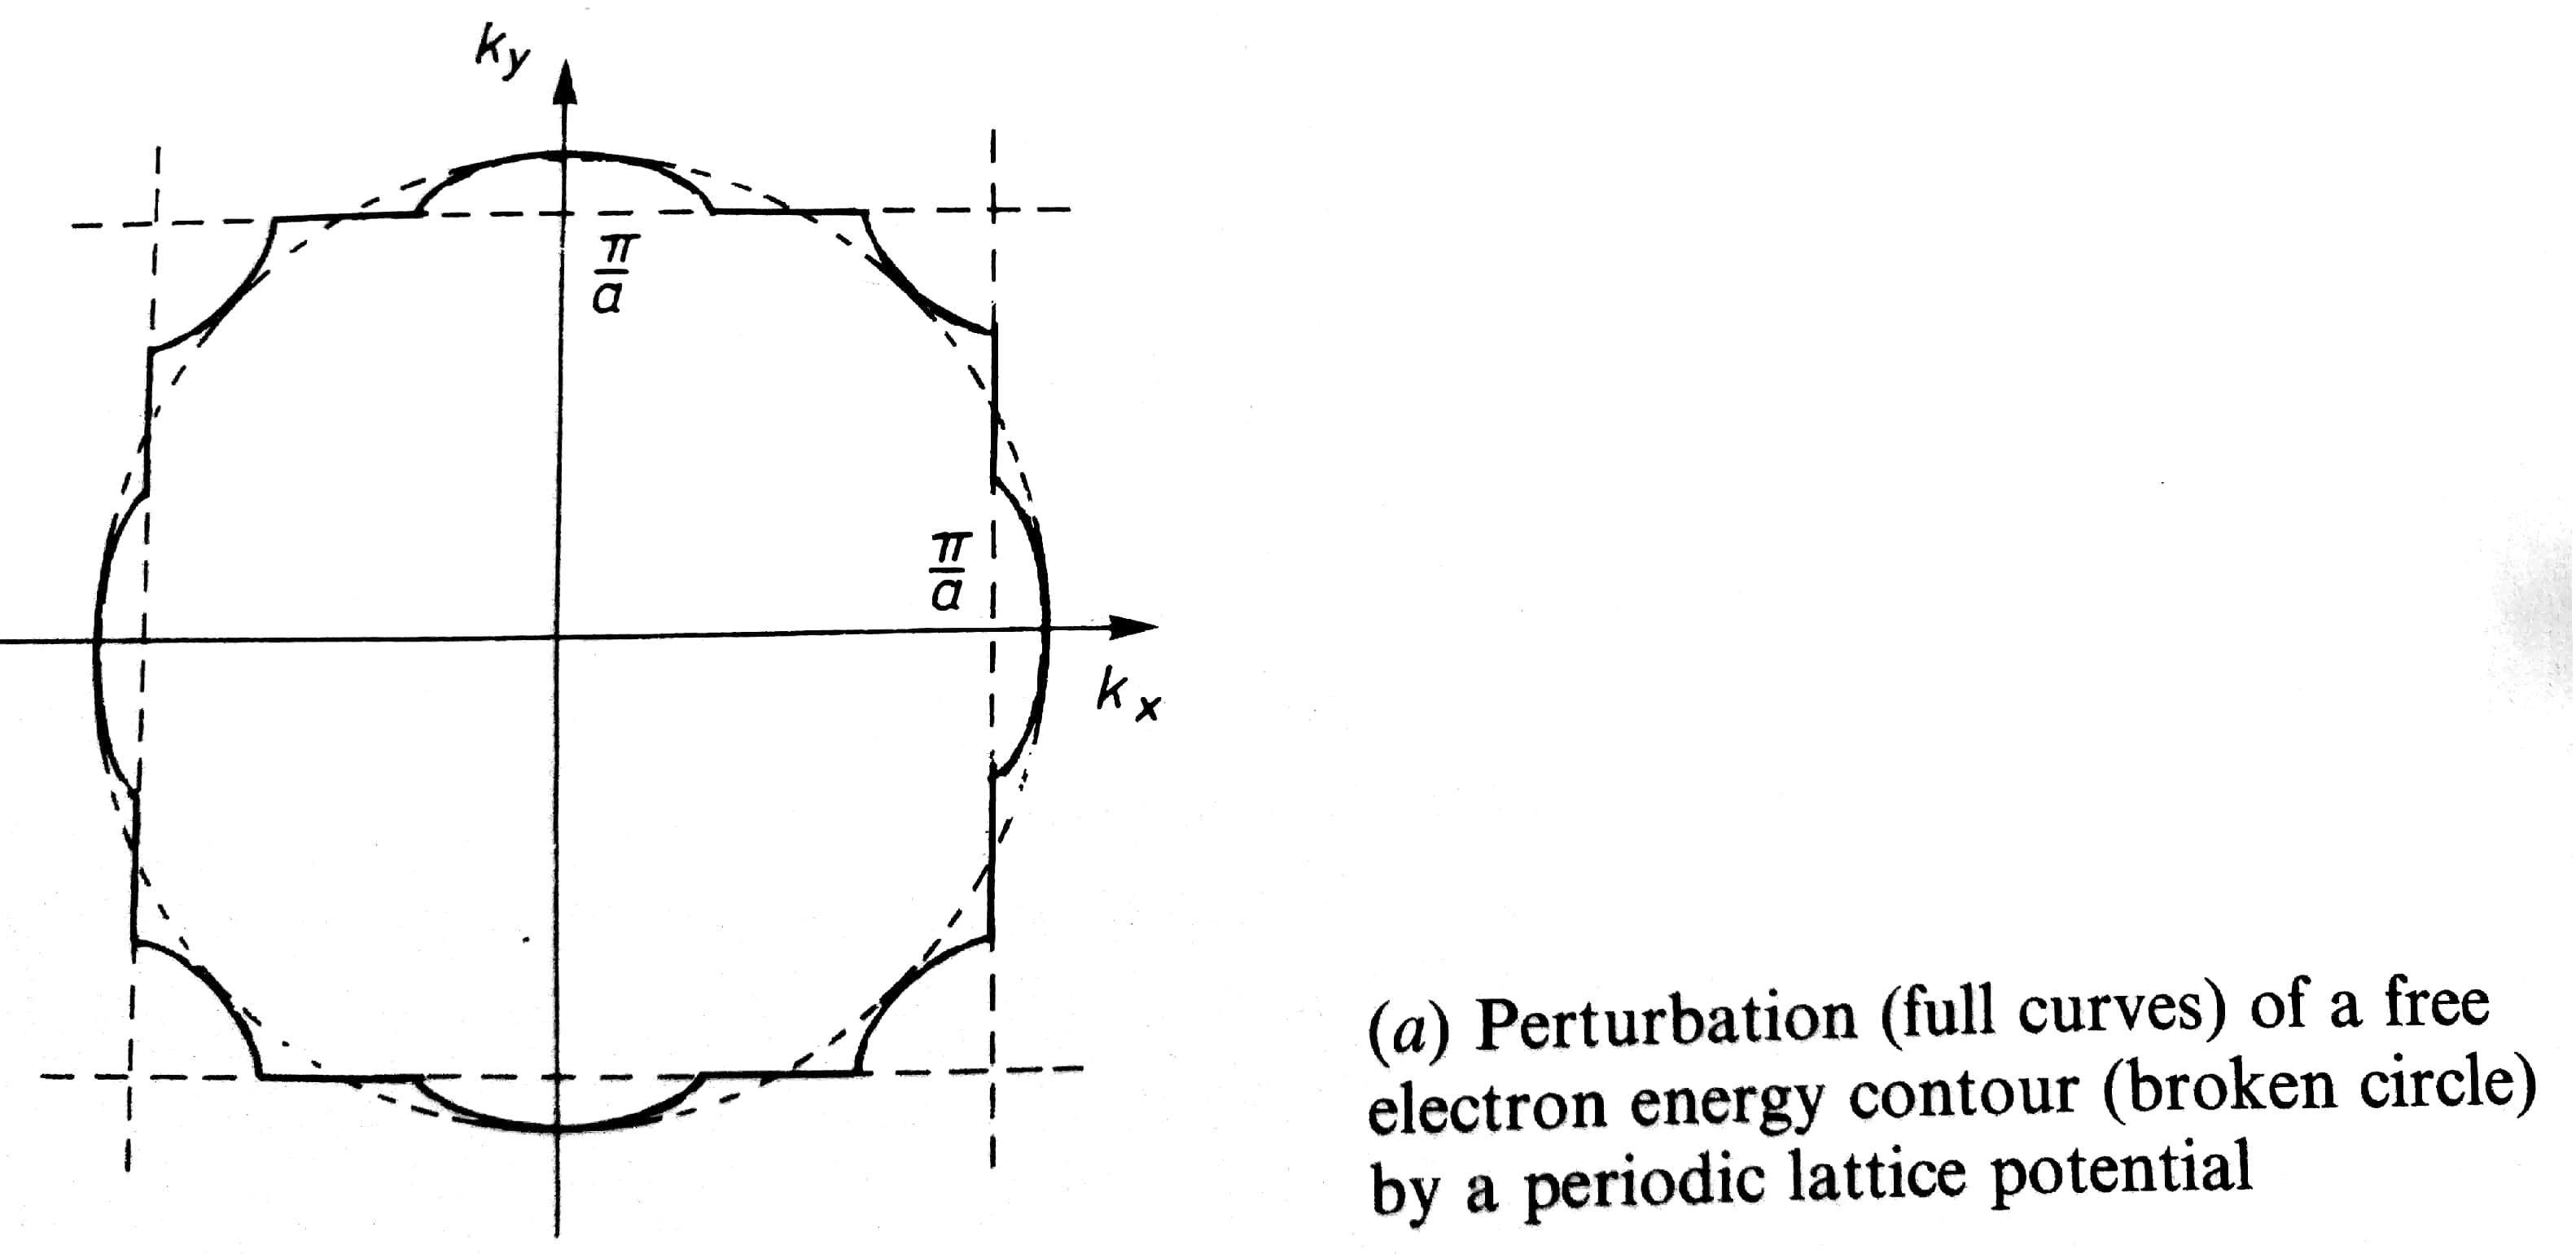
\includegraphics[width=0.7\textwidth]{2d-fermi-perturbated}
	\caption{Copied from Solid State Physics by J.R. Hook and H.E. Hall}
	\label{fig:2d-fermi-perturbated}
\end{figure}
\newpage
So how does this result in overlapping bands? Well look at the corners! The $|\pmb{k}|$ value there is about $\sqrt{2}$ times larger there! Thus for smaller potential we get and overlap of bands. Then electrons can smoothly start occupying states in the second energy band.

To surmise certain features extends to all crystal, no matter the dimensions.
\begin{enumerate}
	\item An odd number of valence electrons in a primitive unit cell leads to metallic behaviour
	\item An even number of valence electrons per primitive unit cell leads to metallic behaviour \emph{if} there is a band overlap, a semiconductor if there is a small band gap, and an insulator if there is a large band gap.
\end{enumerate}

\subsection{The tight binding approach}
The nearly free electron theory has provided even more answer, such as why certain materials are metals and others insulators. It has not, however, been able to give us much insight to the nature of the electron wavefunctions. It also is not suited to describe the covalent bonding by valence electrons in important semiconductor crystals. To further explore the nature of the solid state of matter we look at the tight binding approach!

\subsubsection{Coupled probability amplitudes}
We start, yet again, with the simplest one dimensional crystal we can use, the one dimensional chain of atoms separated by a distance $a$. When atoms are widely separated, the wavefunctions of the valence electrons will be those of isolated atoms. But as the atoms get closer we expect that the electrons will begin to move from one atom to another. We can see this as a transfer of the electron from state $\phi_n$ to the same state for a neighbouring atom $\phi_{n-1}$ or $\phi_{n+1}$. Thus we should be able to write the wavefunction of the electron as a linear combinations of the states $\phi_n$ on the $N$ atoms in the chain
\begin{equation}
	\Psi = \sum^N_{n=1} a_n(t) \phi_n
\end{equation}
The time dependent Shrödinger is cumbersome to calculate. We can use the alternative formulation for quantum mechanics which gives the probability $|c_n(t)|^2$ for finding the electron in state $\phi_n$ at time $t$. $c_n(t)$ is \emph{not} equal to the coefficient $a_n(t)$; however, we wish to find the stationary of the system, and for these the time-dependence of $a_n(t)$ and $c_n(t)$ is the same
\begin{equation}
	a_n \propto c_n \propto e^{-Et/\hslash}
\end{equation}	
where $E$ is the energy of the state. And this alternative formulation(just given here) gives a set of N equations
\begin{equation}
	i\hslash \frac{dc_n}{dt} = Bc_n - Ac_{n-1} - Ac_{n+1}
	\label{eq:alternative-shrodinger}
\end{equation}
And the physical interpretation is of course that the two latter terms represent the changes in $c_n$ due to the proximity or transfer with the neighbouring atom. If these terms are removed we get an expression for an electron at an atom $m$
\[ c_n(0) =
  \begin{cases}
    1 & \quad \text{if } m=n \text{ is even}\\
    0 & \quad \text{otherwise} \\
  \end{cases}
\]
basically the electron sticks to its atom.
\subsubsection{Electron states on a one-dimensional chain}
Solving $c_n$ using equation~\ref{eq:alternative-shrodinger} requires us to assume a solution to solve.Looking at the similarity with the one dimensional chain lattice vibration we know to assume
\begin{equation}
	c_n = C e^{i(kx_n^0 - \omega t)}
\end{equation}
where $x_n^0 = na$ is the equilibrium position of the $n$th atom in the chain. Putting this into equation~\ref{eq:alternative-shrodinger} we get
\begin{equation}
	\hslash \omega e^{i(kna - \omega t)} = Be^{i(kna-\omega t)} - Ae^{i[k(n-1) - \omega t]} - Ae^{i[k(n+1) - \omega t]}
\end{equation}
Knowing that the energy $\epsilon = \hslash \omega$, we cancel some exponential parts and get
\begin{equation}
	\epsilon = B - 2A\cos{(ka)}.
	\label{eq:alternative-shrodinger-energy}
\end{equation}
looking at figure~\ref{fig:tight-bonding} we can see $\epsilon(k)$ plotted. It's worth noting that with more neighbours we would only add harmonics, so it wouldn't change the periodicity of $\epsilon(k)$. With changing values $A$ and $B$ in equation~\ref{eq:alternative-shrodinger-energy} we can obtain other energy bands\footnote{How we solve for these values is not given}, and how these are represented in different ways are showed in figure~\ref{fig:zone-schemes}. Note that each band goes through the solid itself. Thus to obtain the energy levels of electrons corresponding to one atom one just looks at the reduced scheme.
\begin{figure}[!ht] 
	\centering
	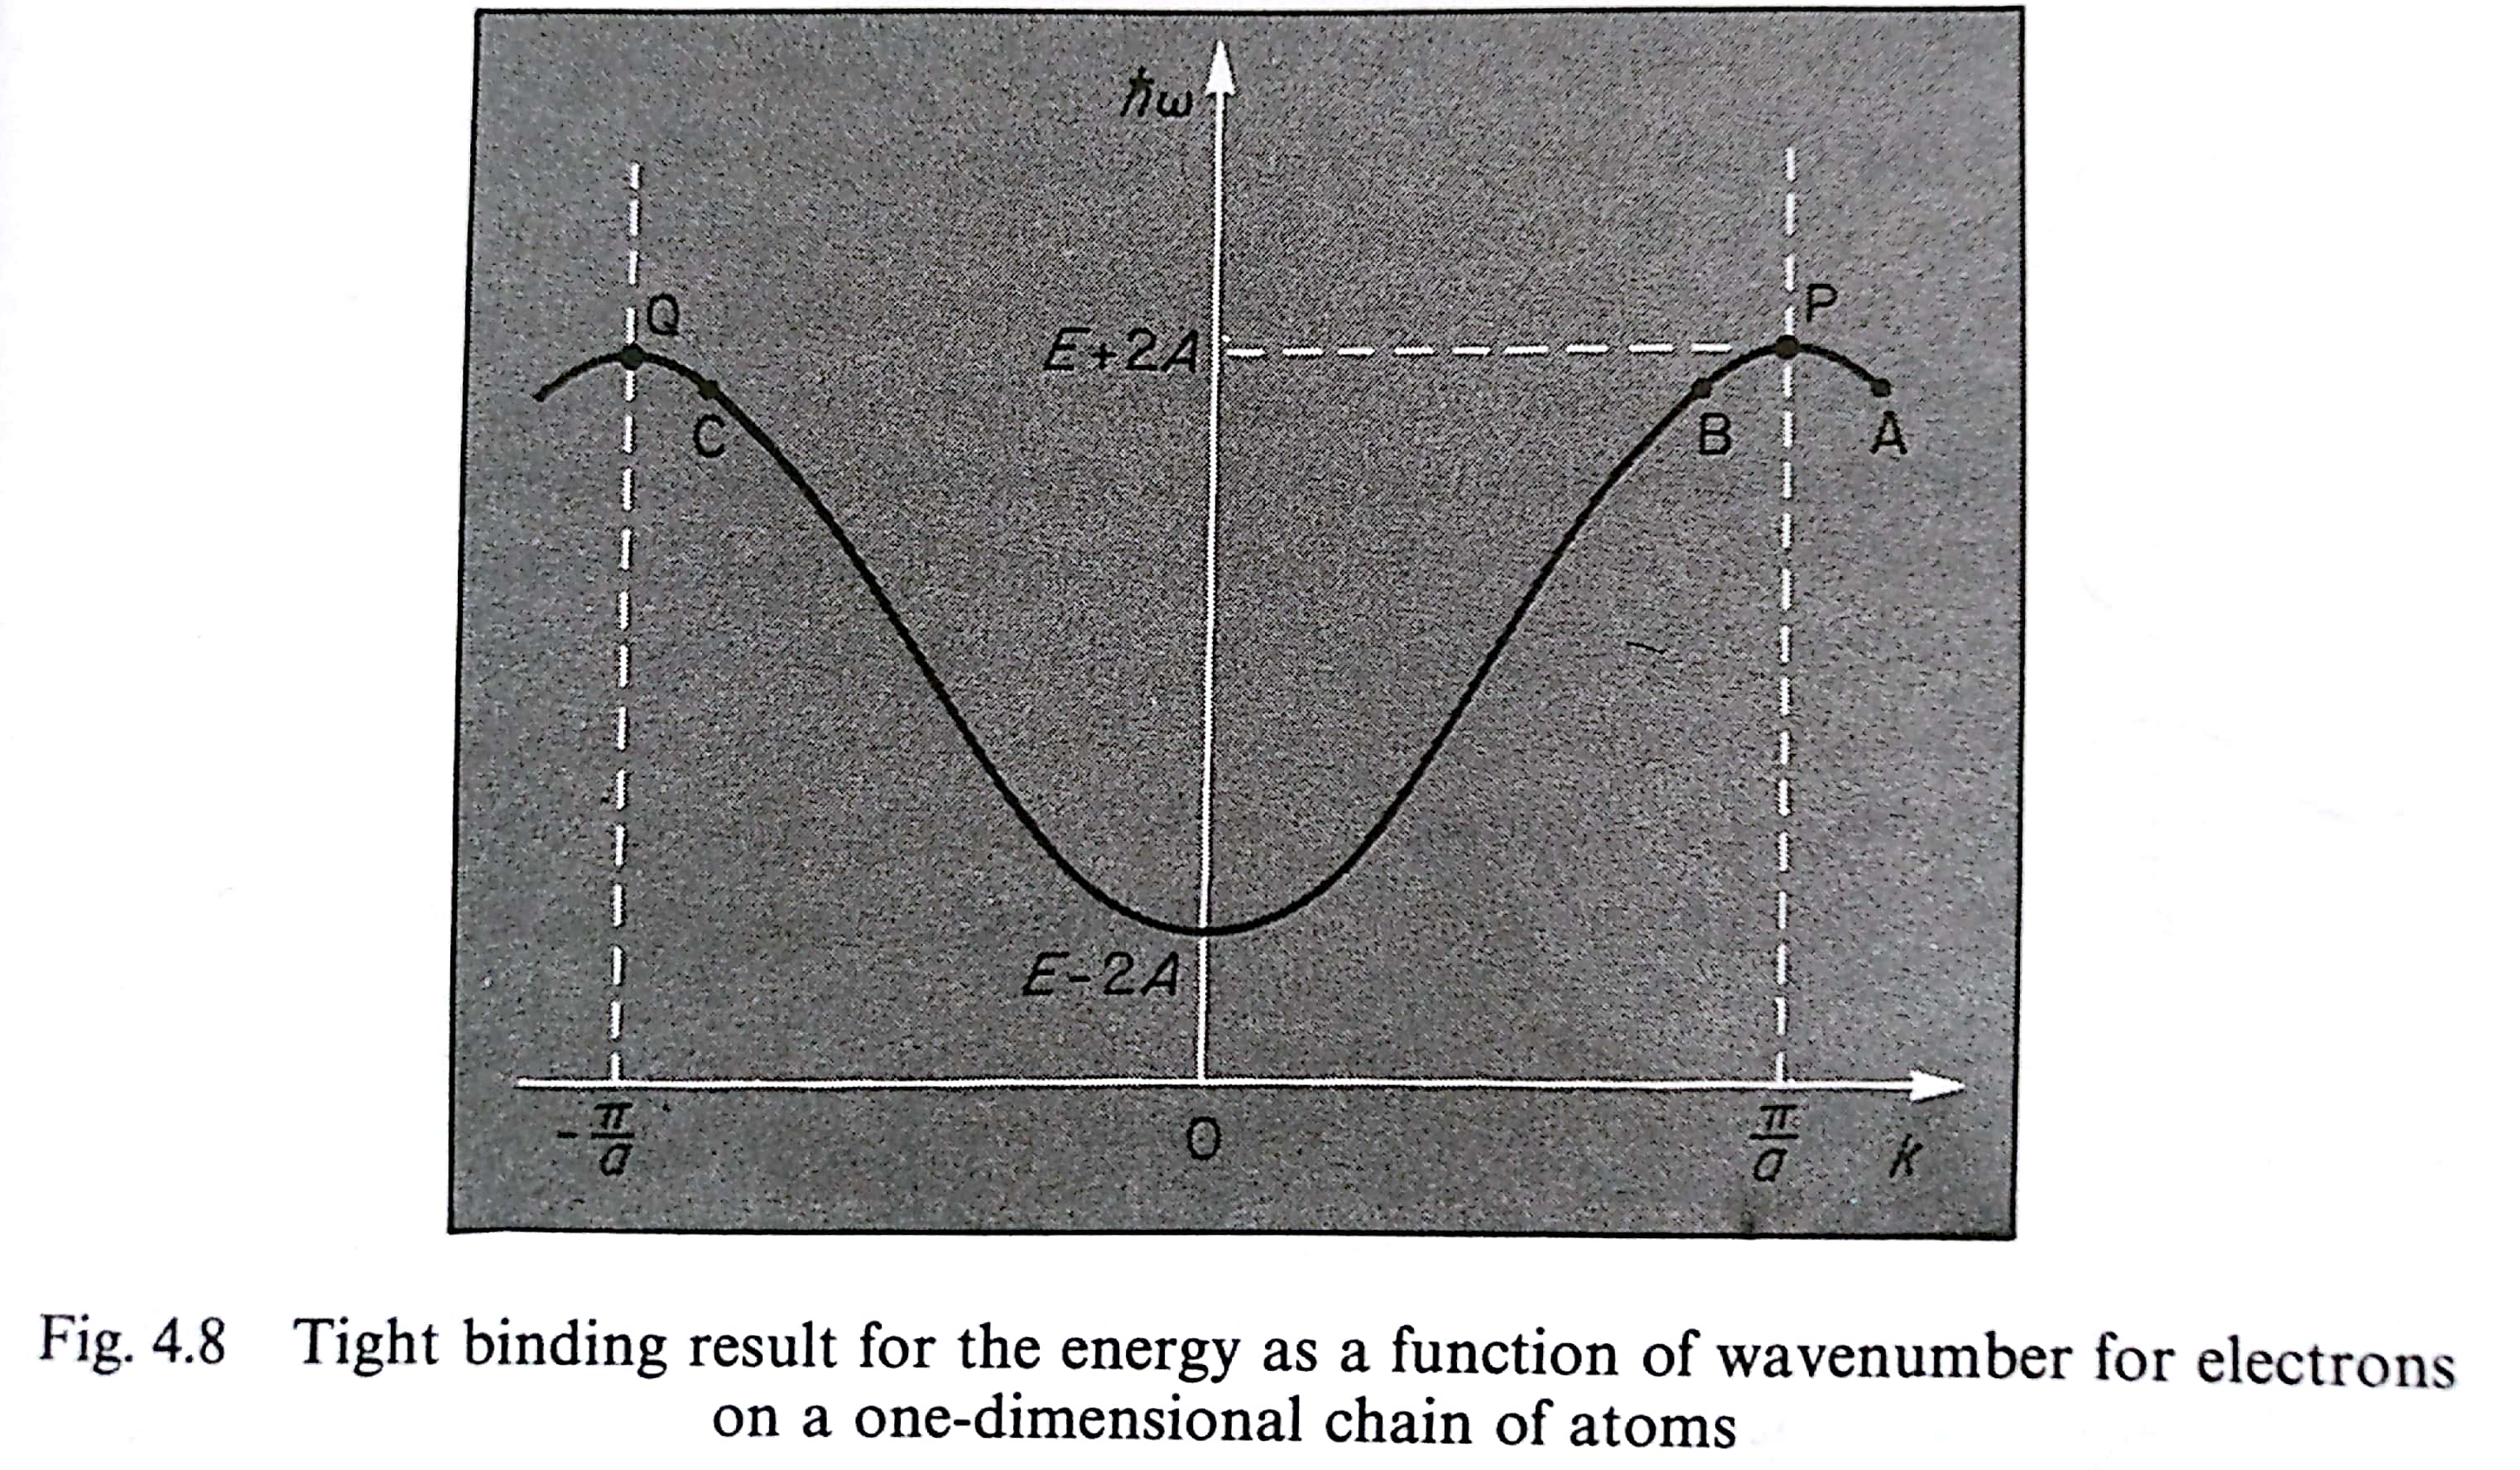
\includegraphics[width=0.7\textwidth]{tight-bonding}
	\caption{Copied from Solid State Physics by J.R. Hook and H.E. Hall}
	\label{fig:tight-bonding}
\end{figure}
\begin{figure}[!ht]
	\centering
	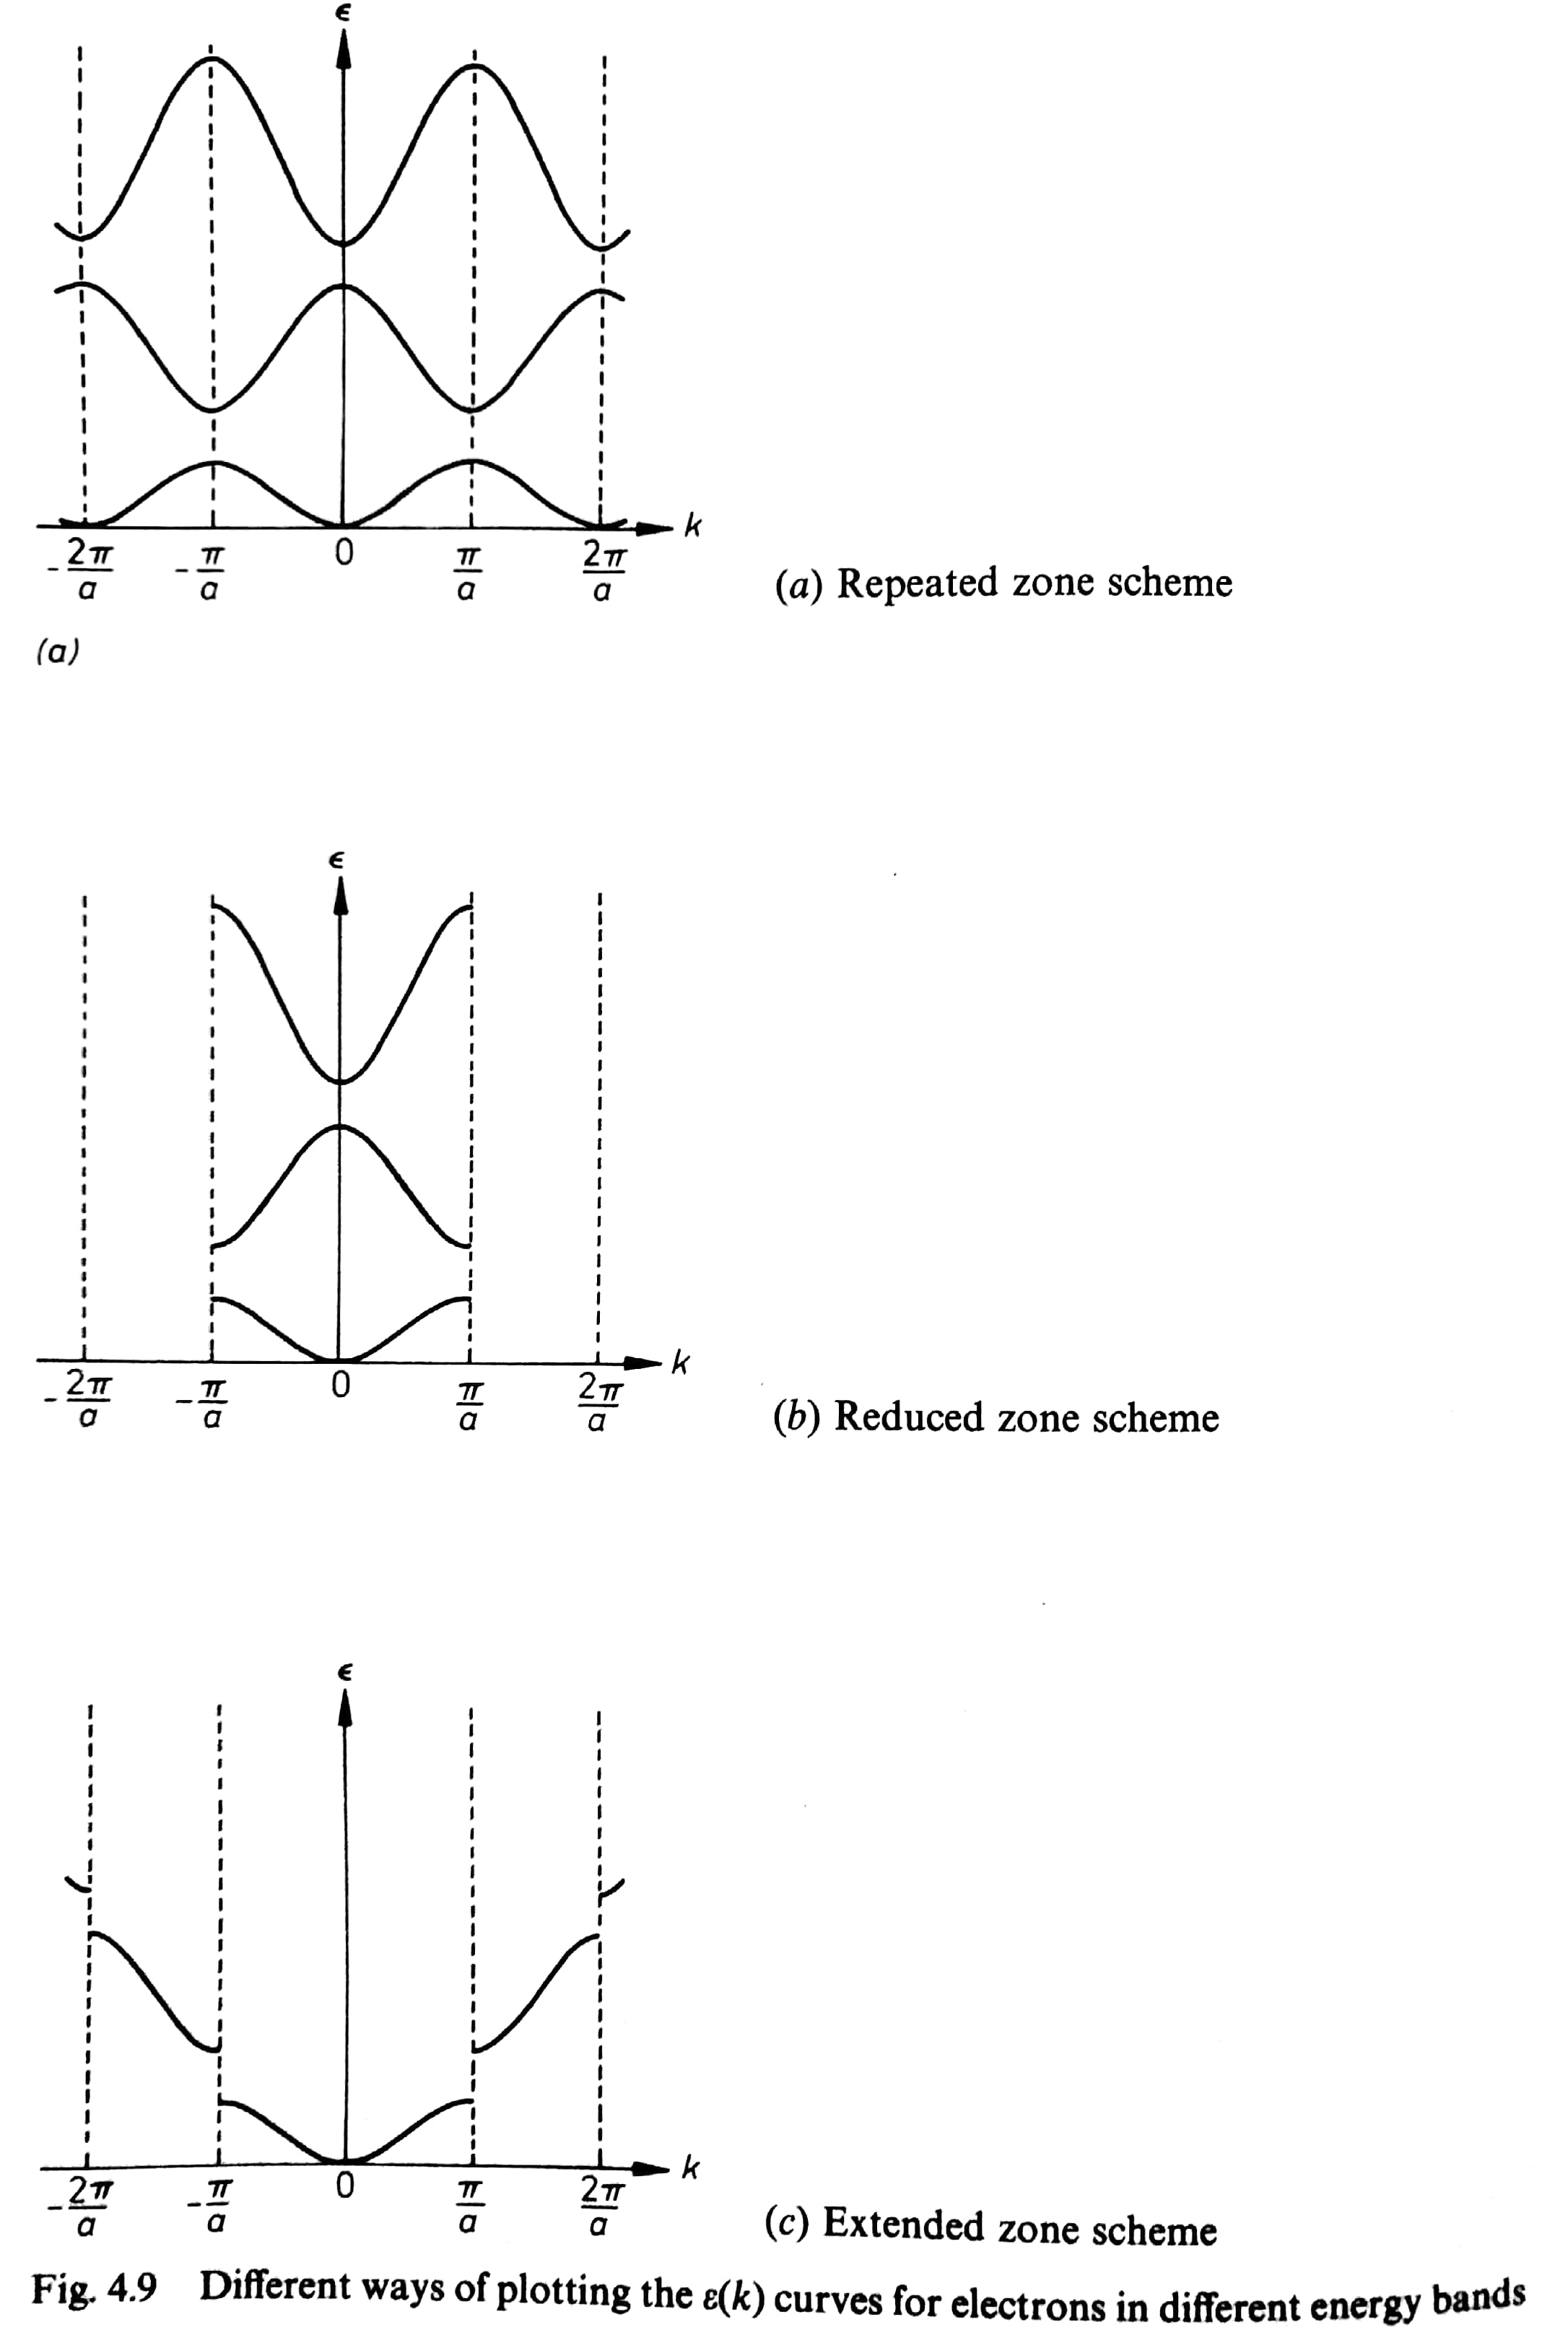
\includegraphics[width=0.7\textwidth]{zone-schemes}
	\caption{Copied from Solid State Physics by J.R. Hook and H.E. Hall}
	\label{fig:zone-schemes}
\end{figure}
On pages 119-121 in the book we have some more real world examples of potentials which could be interesting to look through if interested.

\newpage
\subsubsection{Electron states in diamond, silicon and germanium}
Using the same calculations for more complex structures in three dimensions, for example diamonds, we need to modify our wavefunction as 
\begin{equation}
	\Psi = \sum_n C e^{i(\pmb{k} \cdot \pmb{r}_n - \omega t)} \phi_n
\end{equation}
where the sum is over the lattice points at position $\pmb{r}_n$, thus the standing waves at a given value $\pmb{k}$ is standing waves determined by the periodicity of the lattice. The wave function $\phi_n$ must thus be an orbital appropriate to the basis of the atoms associated with each lattice point, rather then with an isolated atom. Further application of this is showed in the book on pages 122-124.

\subsubsection{Band structure effective masses}
Time to consider the effective mass again! If we look at the electrons wavepacket now instead of an electron, we could find out the effective mass of an electron instead of an electron itself. We will construct a wavepacket from one energy band, centred on energy $\epsilon$ and the wavenumber $k$. We then want to calculate the motion of the wavepacket in the time interval $\partial t$. To  do this we assume
\begin{enumerate}
	\item The velocity of the wavepacket is the group velocity
		\begin{equation}
			v = \frac{d \omega}{dk} = \frac{1}{\hslash} \frac{d \epsilon}{d k}
		\end{equation}
	\item The motion of the wavepacket resembles that of a classical particle in that its \emph{total} energy remains constant. Thus
	\begin{equation}
		\partial \epsilon = - eE \partial x
	\end{equation}
\end{enumerate}
Using these equations we can derive the equation of motion in two forms.
\begin{equation}
	\partial k = \partial k = \frac{dk}{d\epsilon} \partial e = \frac{1}{\hslash v} \partial \epsilon
\end{equation}
and 
\begin{equation}
	\frac{dk}{dt} = \frac{1}{\hslash v} \frac{d \epsilon}{dt} = -\frac{eE}{\hslash}
\end{equation}
or more concisely
\begin{equation}
	\hslash \frac{dk}{dt} = -eE
\end{equation}
By massaging these equations together\footnote{Only algebra, is described in the book on page 126} we get the equation
\begin{equation}
	m_e \frac{dv}{dt} = -eE
\end{equation}
where
\begin{equation}
	m_e = \hslash^2 / \frac{d^2\epsilon}{dk^2}
\end{equation}
And we have our effective mass! This can be used to obtain more exact values when used in conjuction with the equation previously derived in the section about the free electron gas. 

If one want to use this for calculating the heat capacity, one must remember to only use values that exists on the Fermi surface.

\newpage
\section{Semiconductors}
\subsection{Introduction}
For certain materials the highest occupied energy is completely full at zero temperature, this band is called the \textbf{valence band}, and the lowest unoccupied band is called the \textbf{conduction band}. For semiconductor the behavior is mostly related to the electron states close to the top of the valence band and t he bottom of the conduction band. We have these bands depicted in figure~\ref{fig:semiconductor-band}. Since we're dealing with states close to a maximum or minimum of energy we can take t he dispersion curve $\epsilon(k)$ to be parabolic to a good approximation, we get
\begin{align}
	\text{Conduction band} \quad &\epsilon = E_g + \frac{\hslash^2 k^2}{2m_e} \\
	\text{Valence band} \quad &\epsilon = - \frac{\hslash^2 k^2}{2m_h} \\
\end{align}
To calculate all the valance band electrons in order to figure out the properties of a nearly full valence band can be cumbersome. But there exists an alternative! We can look at the holes left behind. This hole can be looked at as a particle with positive charge $|e|$, positve mass $m_h$ and energy $\hslash^2 k^2/2m_h$, positve mass $m_h$ and energy $\hslash^2 k^2/2m_h$.
\begin{figure}[!ht]
	\centering
	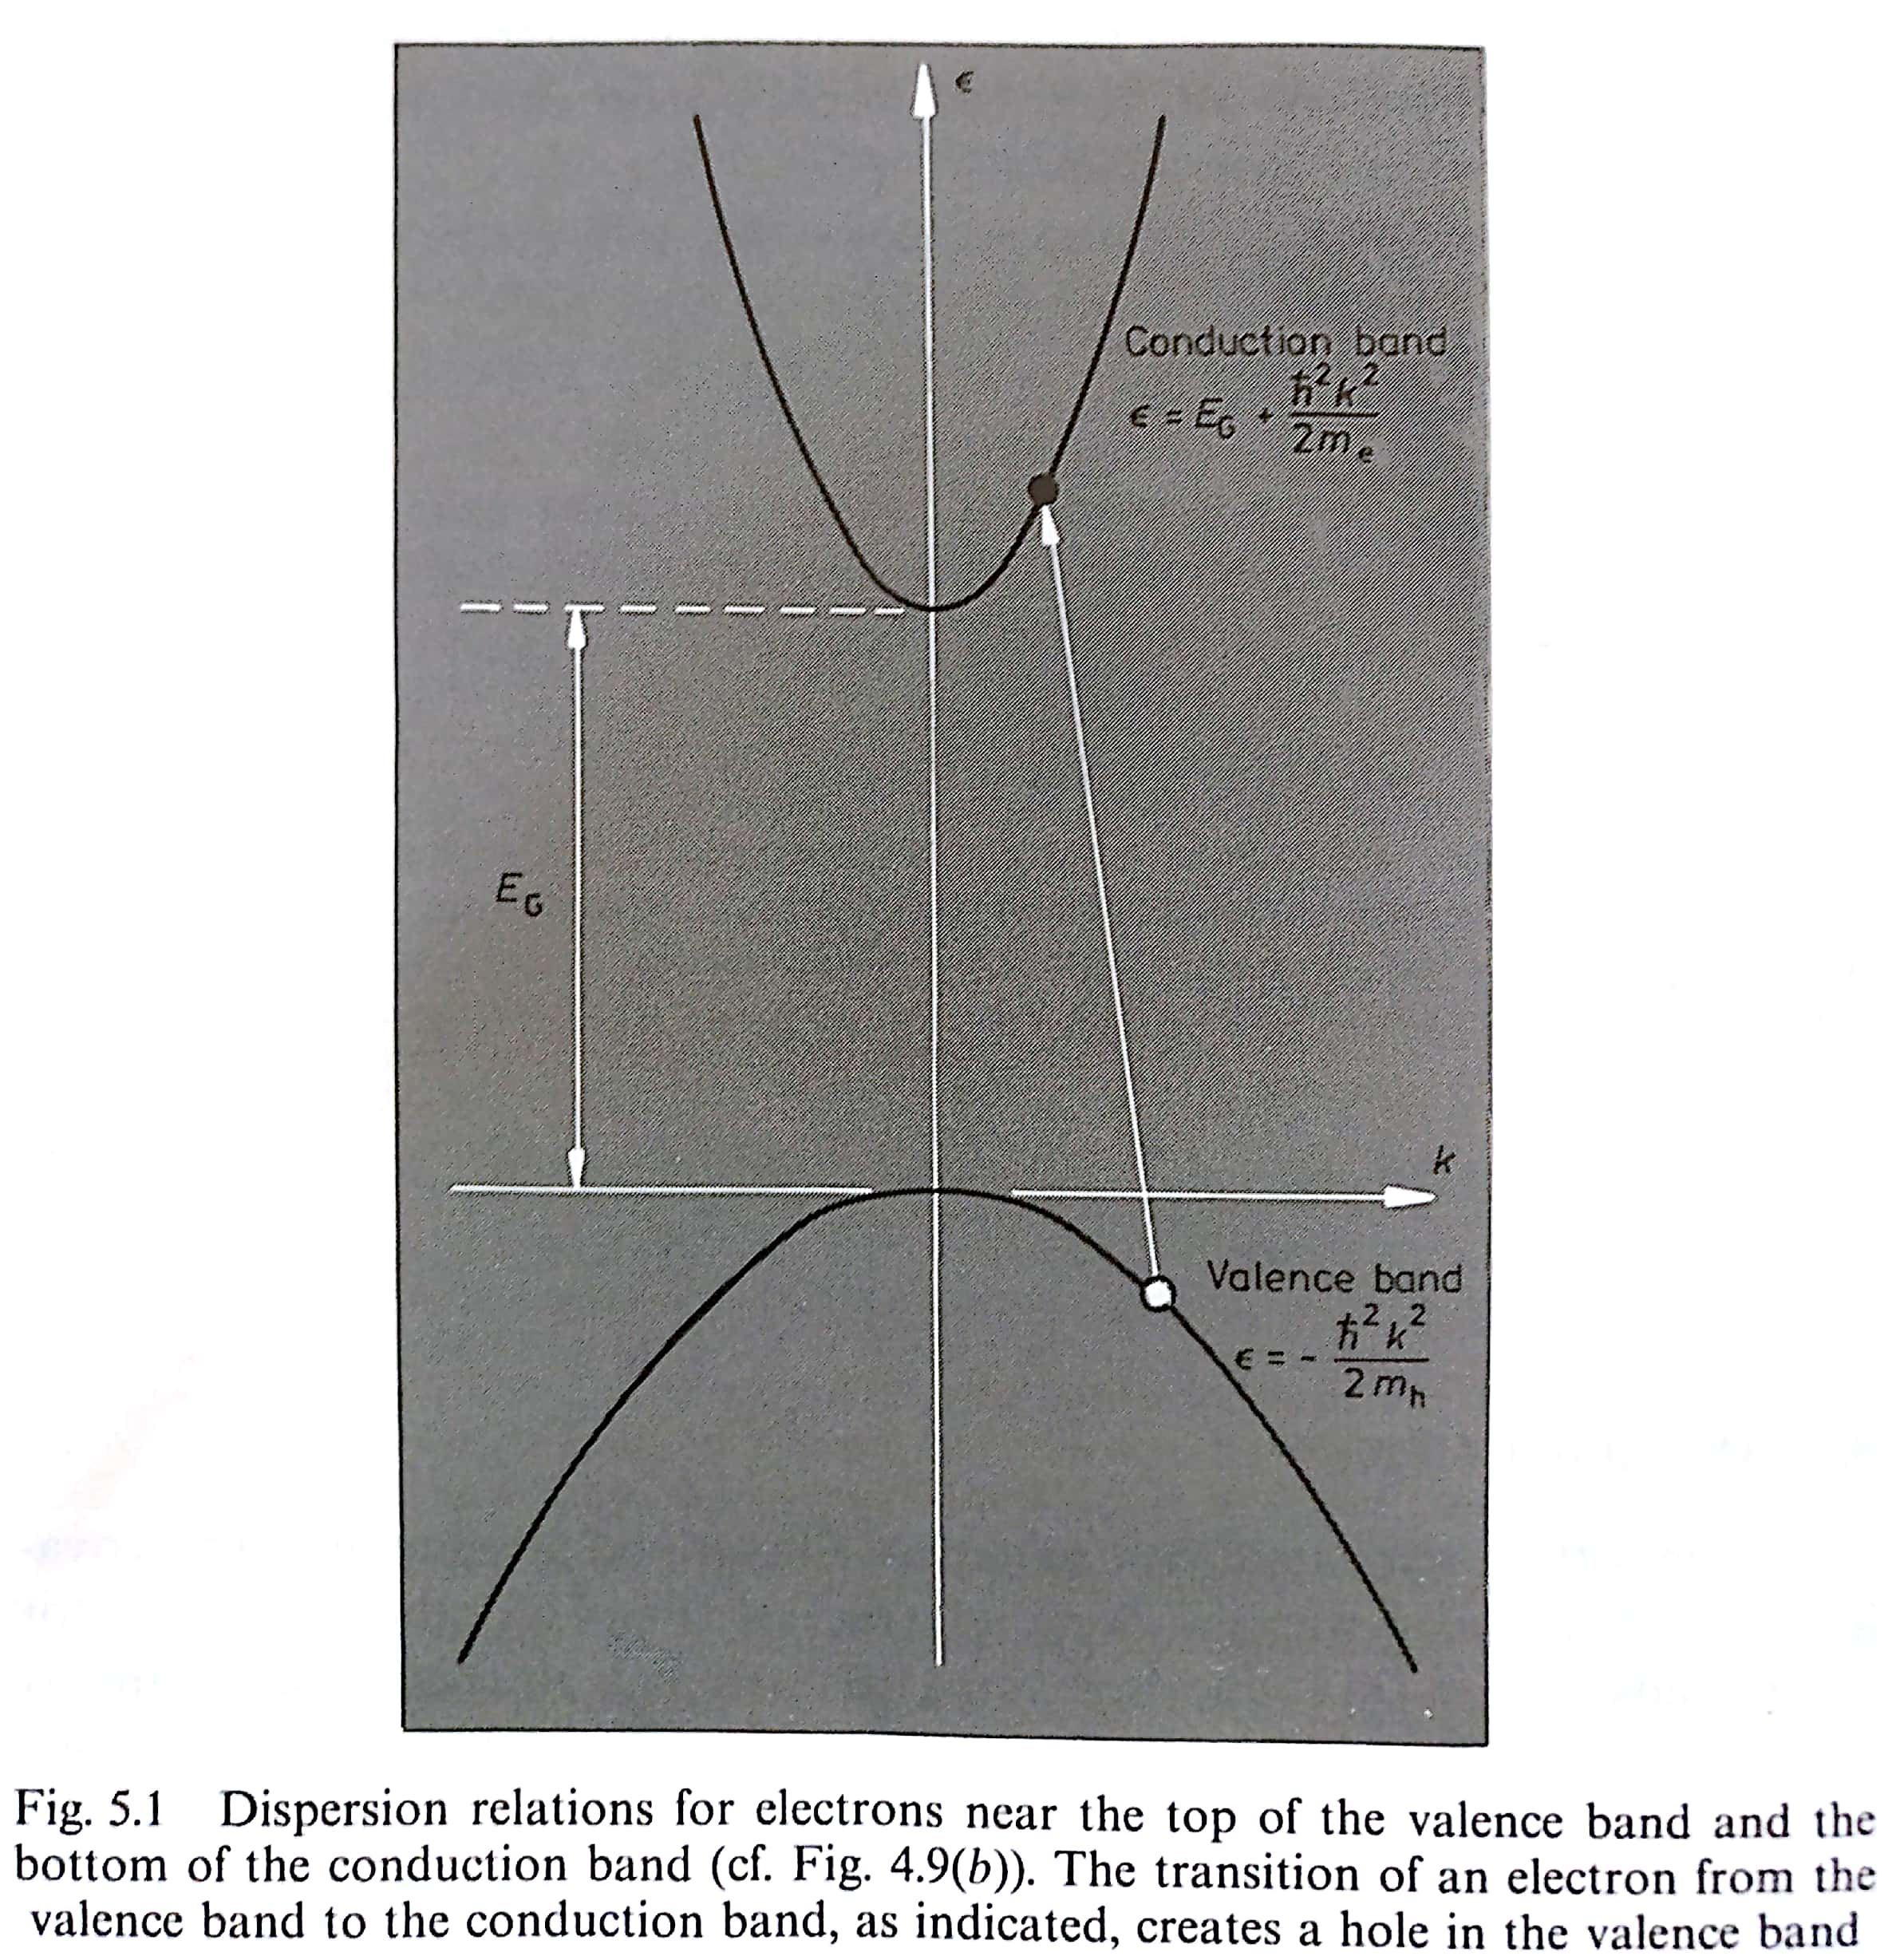
\includegraphics[width=0.7\textwidth]{semiconductor-band}
	\caption{Copied from Solid State Physics by J.R. Hook and H.E. Hall}
	\label{fig:semiconductor-band}
\end{figure}
\subsection{Holes}
The energy of a hole in state $\pmb{k}$ must be the opposite of the energy for an electron.
\begin{equation}
	\epsilon_h q \frac{\hslash^2 k^2}{2m_h}
\end{equation}
Similarly the electron momentum $\hslash \pmb{k}$ must also be reversed
\begin{equation}
	\pmb{p}_h = -\hslash \pmb{k}
\end{equation}

In the book there is a bit more development on all arguments here but for holes we have a similar equation of motion as for electrons, namely
\begin{equation}
	m_h(\frac{d\pmb{v}_h}{dt} + \frac{\pmb{v}_h}{\tau_h}) = e(\pmb{E} + \pmb{v}_h \times \pmb{B}).
\end{equation}
and to tie the sack together we note that a current going through a full band, is in reality nothing\ldots nothing changes! So we look at the reverse current created by the positive charge from the hole instead. So the current $\pmb{j} = - (-e) \pmb{v}$, where $pmb{v}$ is the group velocity of the electron, same as that of a hole in the same state. The current thus ends up being $e\pmb{v}_h$. Since the total current can be written as the sum of the contributions from the electrons in t he conduction band and holes in the valence band, these are referred to as the \textbf{charge carriers} in the semiconductor.
\subsection{Methods of providing electrons and holes}

\subsubsection{Donor and acceptor impurities}
If we have a crystal with a full valence band but empty conduction band, we have an insulator. We can however add impuruties to change the properties of the material. If we create a substitutional impurity\footnote{one atom takes the place of where another would have been} with an atom with an extra valence electron, we all of a sudden have one more electron that needs somewhere to be. What we then do is to treat this electron as an electron orbiting a hydrogen atom. This approximation is good if the impurities are so spread out in the crystal that they don't interact with each other. This creates a new Donor impurity level, which represents a new energy level which is much closer to the conduction band then the valence band is. This effect is depicted in figure~\ref{fig:impurities}, where we have the donor level indicating the much lower energy to get some electrons into the conduction band.
\begin{figure}[!ht]
	\centering
	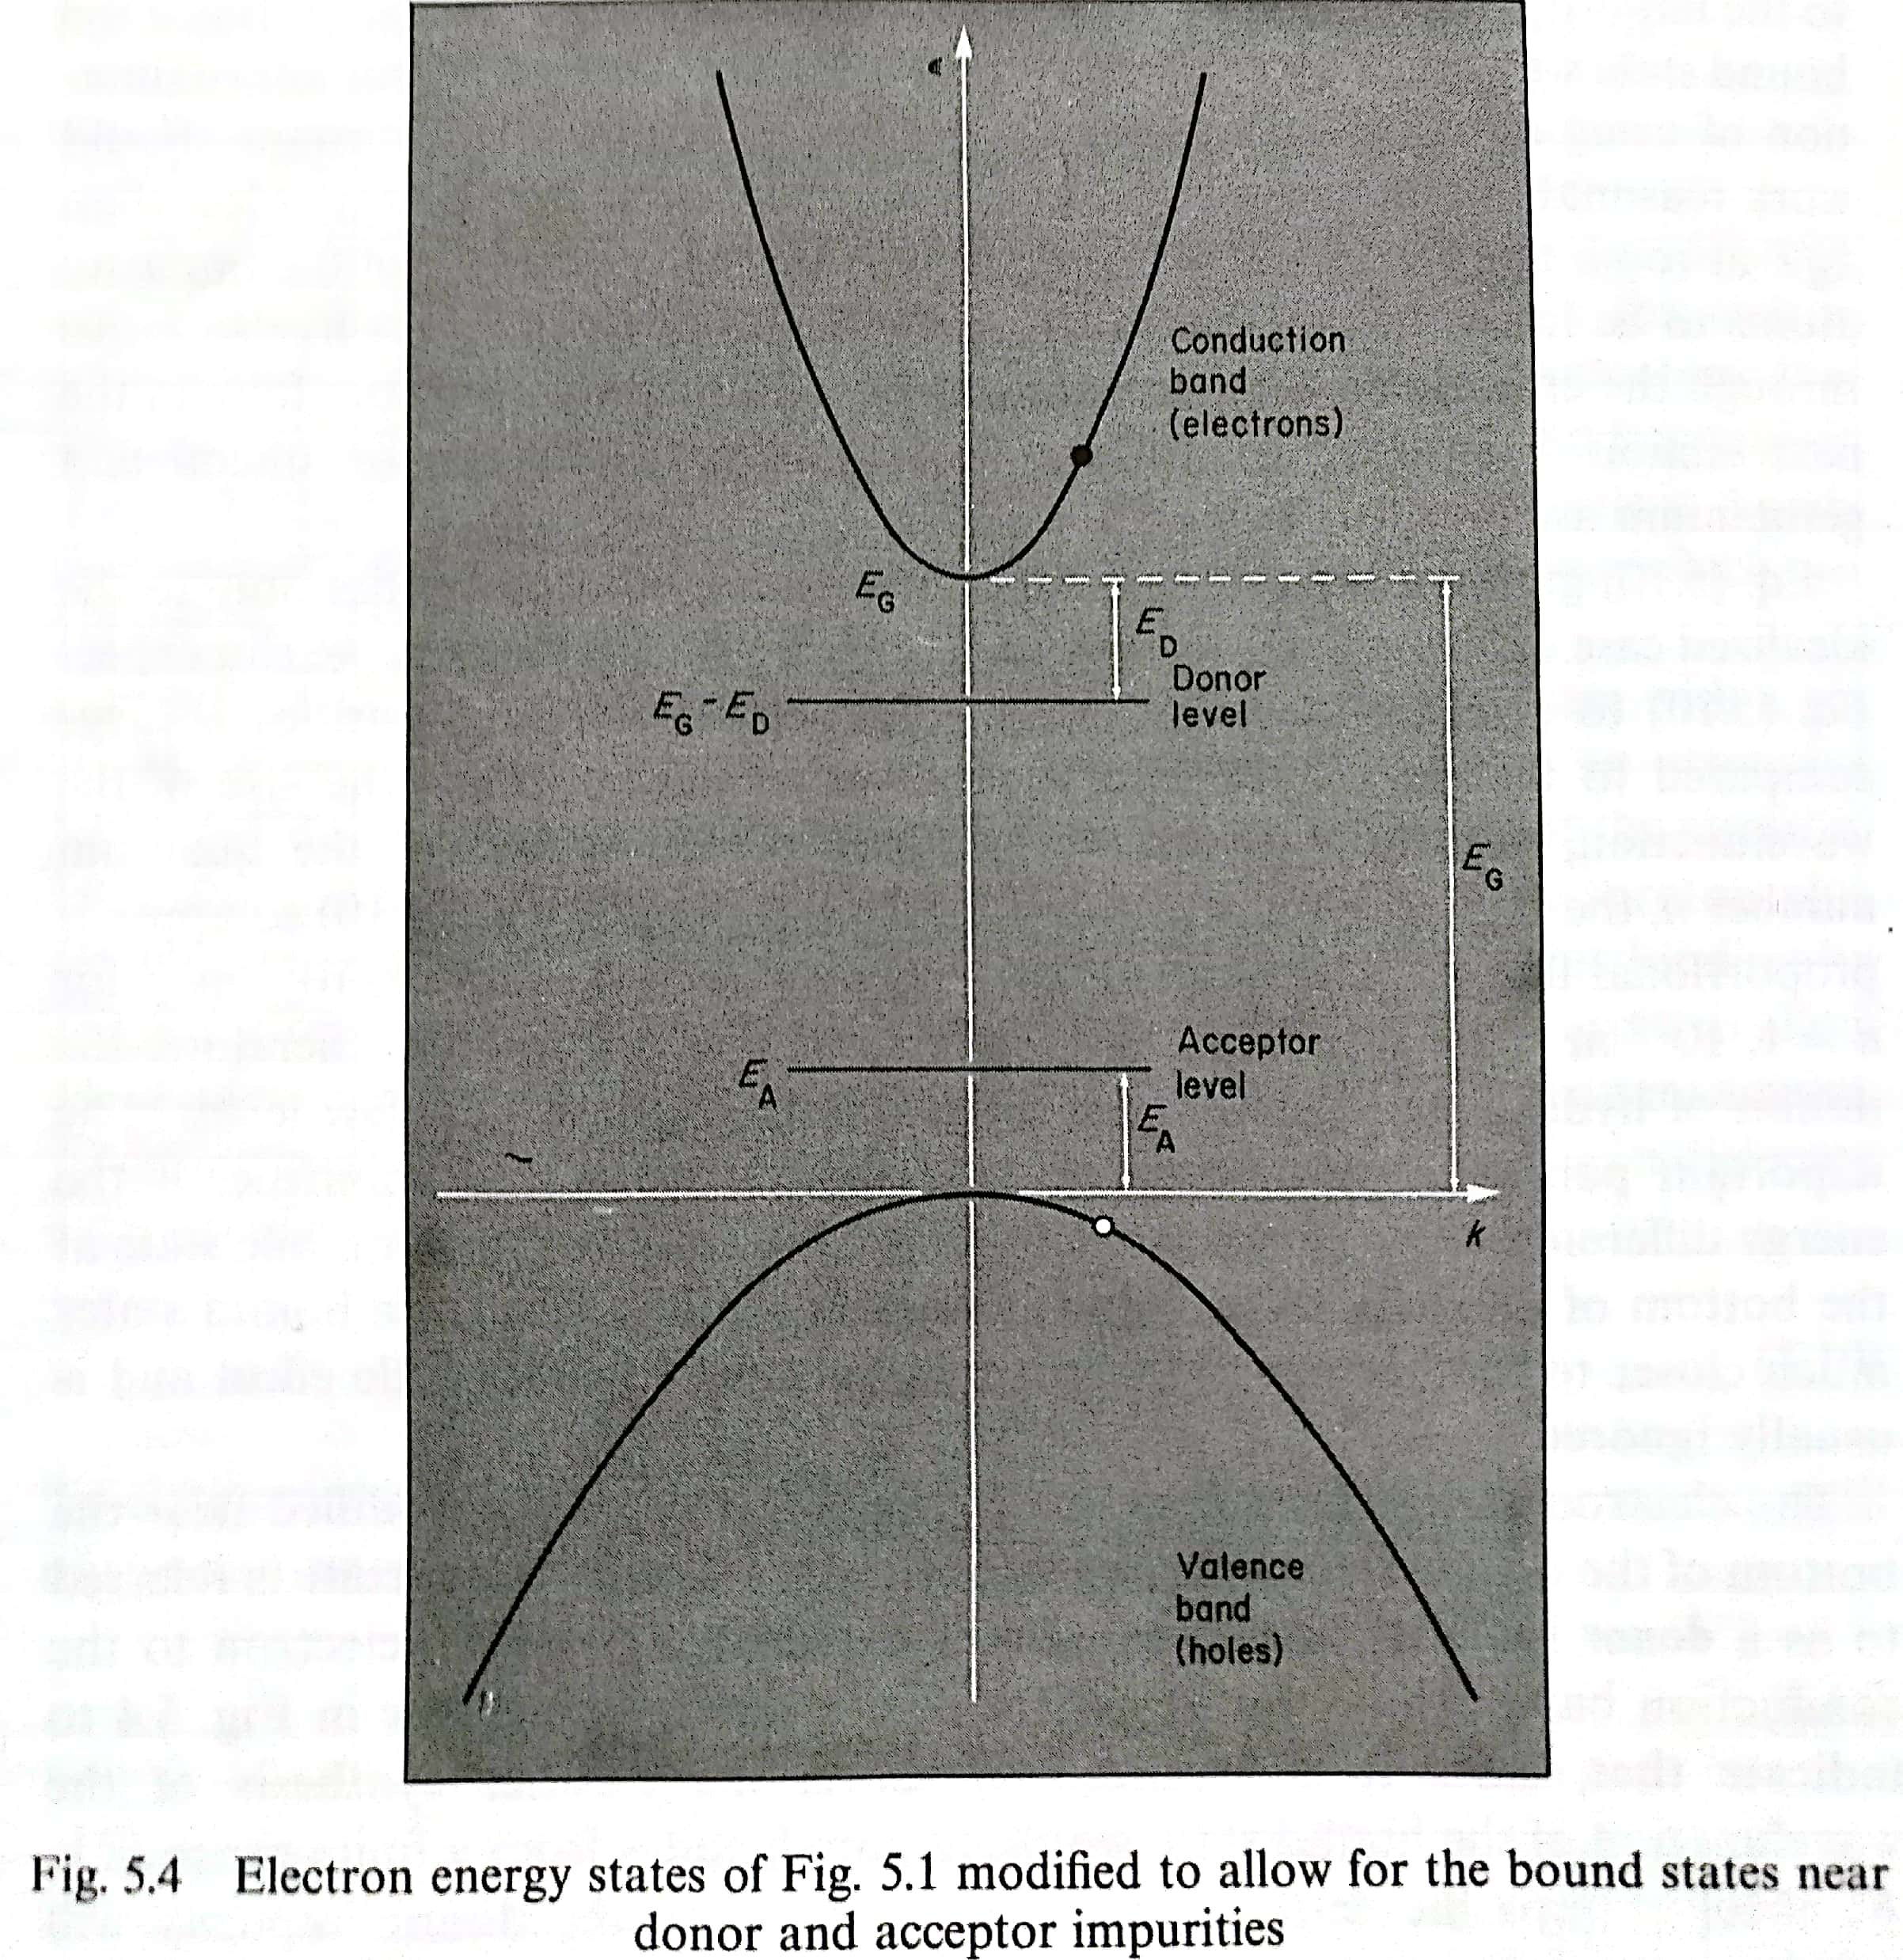
\includegraphics[width=0.7\textwidth]{impurities}
	\caption{Copied from Solid State Physics by J.R. Hook and H.E. Hall}
	\label{fig:impurities}
\end{figure}
Something that can be seen in figure~\ref{fig:impurities} is the acceptor level. Basically this is the reverse effect when you add an impurity with one less electron. This create a state in which an electron can live, thus creating a hole in the valence band. This is another way to make material conductive. Note that all this is derived in pages 136-138 in the book under the assumption that the impurities are very far away from each other.
\newpage
\subsubsection{Thermal excitation of carriers}
We want to calculate the number of charge carries at any temperature $T$. So a good place to start is the Fermi distribution function which tells us the probability of occupation of a state of energy $\epsilon$
\begin{equation}
f(\epsilon, T) = \frac{1}{e^{(\epsilon - \mu)/k_B T} + 1}.
\end{equation}
With that we also need the density of states!
\begin{align}
	\text{Conduction band} \quad & g(\epsilon) = \frac{V}{2\pi^2 \hslash^3} (2m_e)^{3/2}(\epsilon - E_G)^{1/2} \\
	\text{Valence band} \quad &g(\epsilon) = \frac{V}{2\pi^2 \hslash^3} (2m_h)^{3/2}(-\epsilon)^{1/2} \\
\end{align}
We have plotted these functions in figure~\ref{fig:fermi-level}. As we can see the Fermi distribution has a steep fall of at what's called the Fermi level. This drop off depends highly on the value of the chemical potential $\mu$. We refer to the Fermi level when the distribution depends on $\mu(T)$ and call it the Fermi energy when $\mu(0)$. We use this property to estimate the Fermi distribution in the conduction band to be
\begin{equation}
	f(\epsilon) \approx \frac{1}{e^{(\epsilon-\mu)/k_B T}} = e^{(\mu - \epsilon)/k_B T}
\end{equation}
So to find the number of electrons per unit volume in the conduction band we integrate!
\begin{equation}
	n = \frac{1}{V} \int^\infty_{E_G} f(\epsilon)g(\epsilon) d \epsilon = N_C e^{(\mu - E_G)/k_B T}
	\label{eq:concentration-electrons}
\end{equation}
where 
\begin{equation}
	N_C = 2(\frac{2\pi m_e k_B T}{h^2})^{3/2}.
\end{equation}
\begin{figure}[!ht]
	\centering
	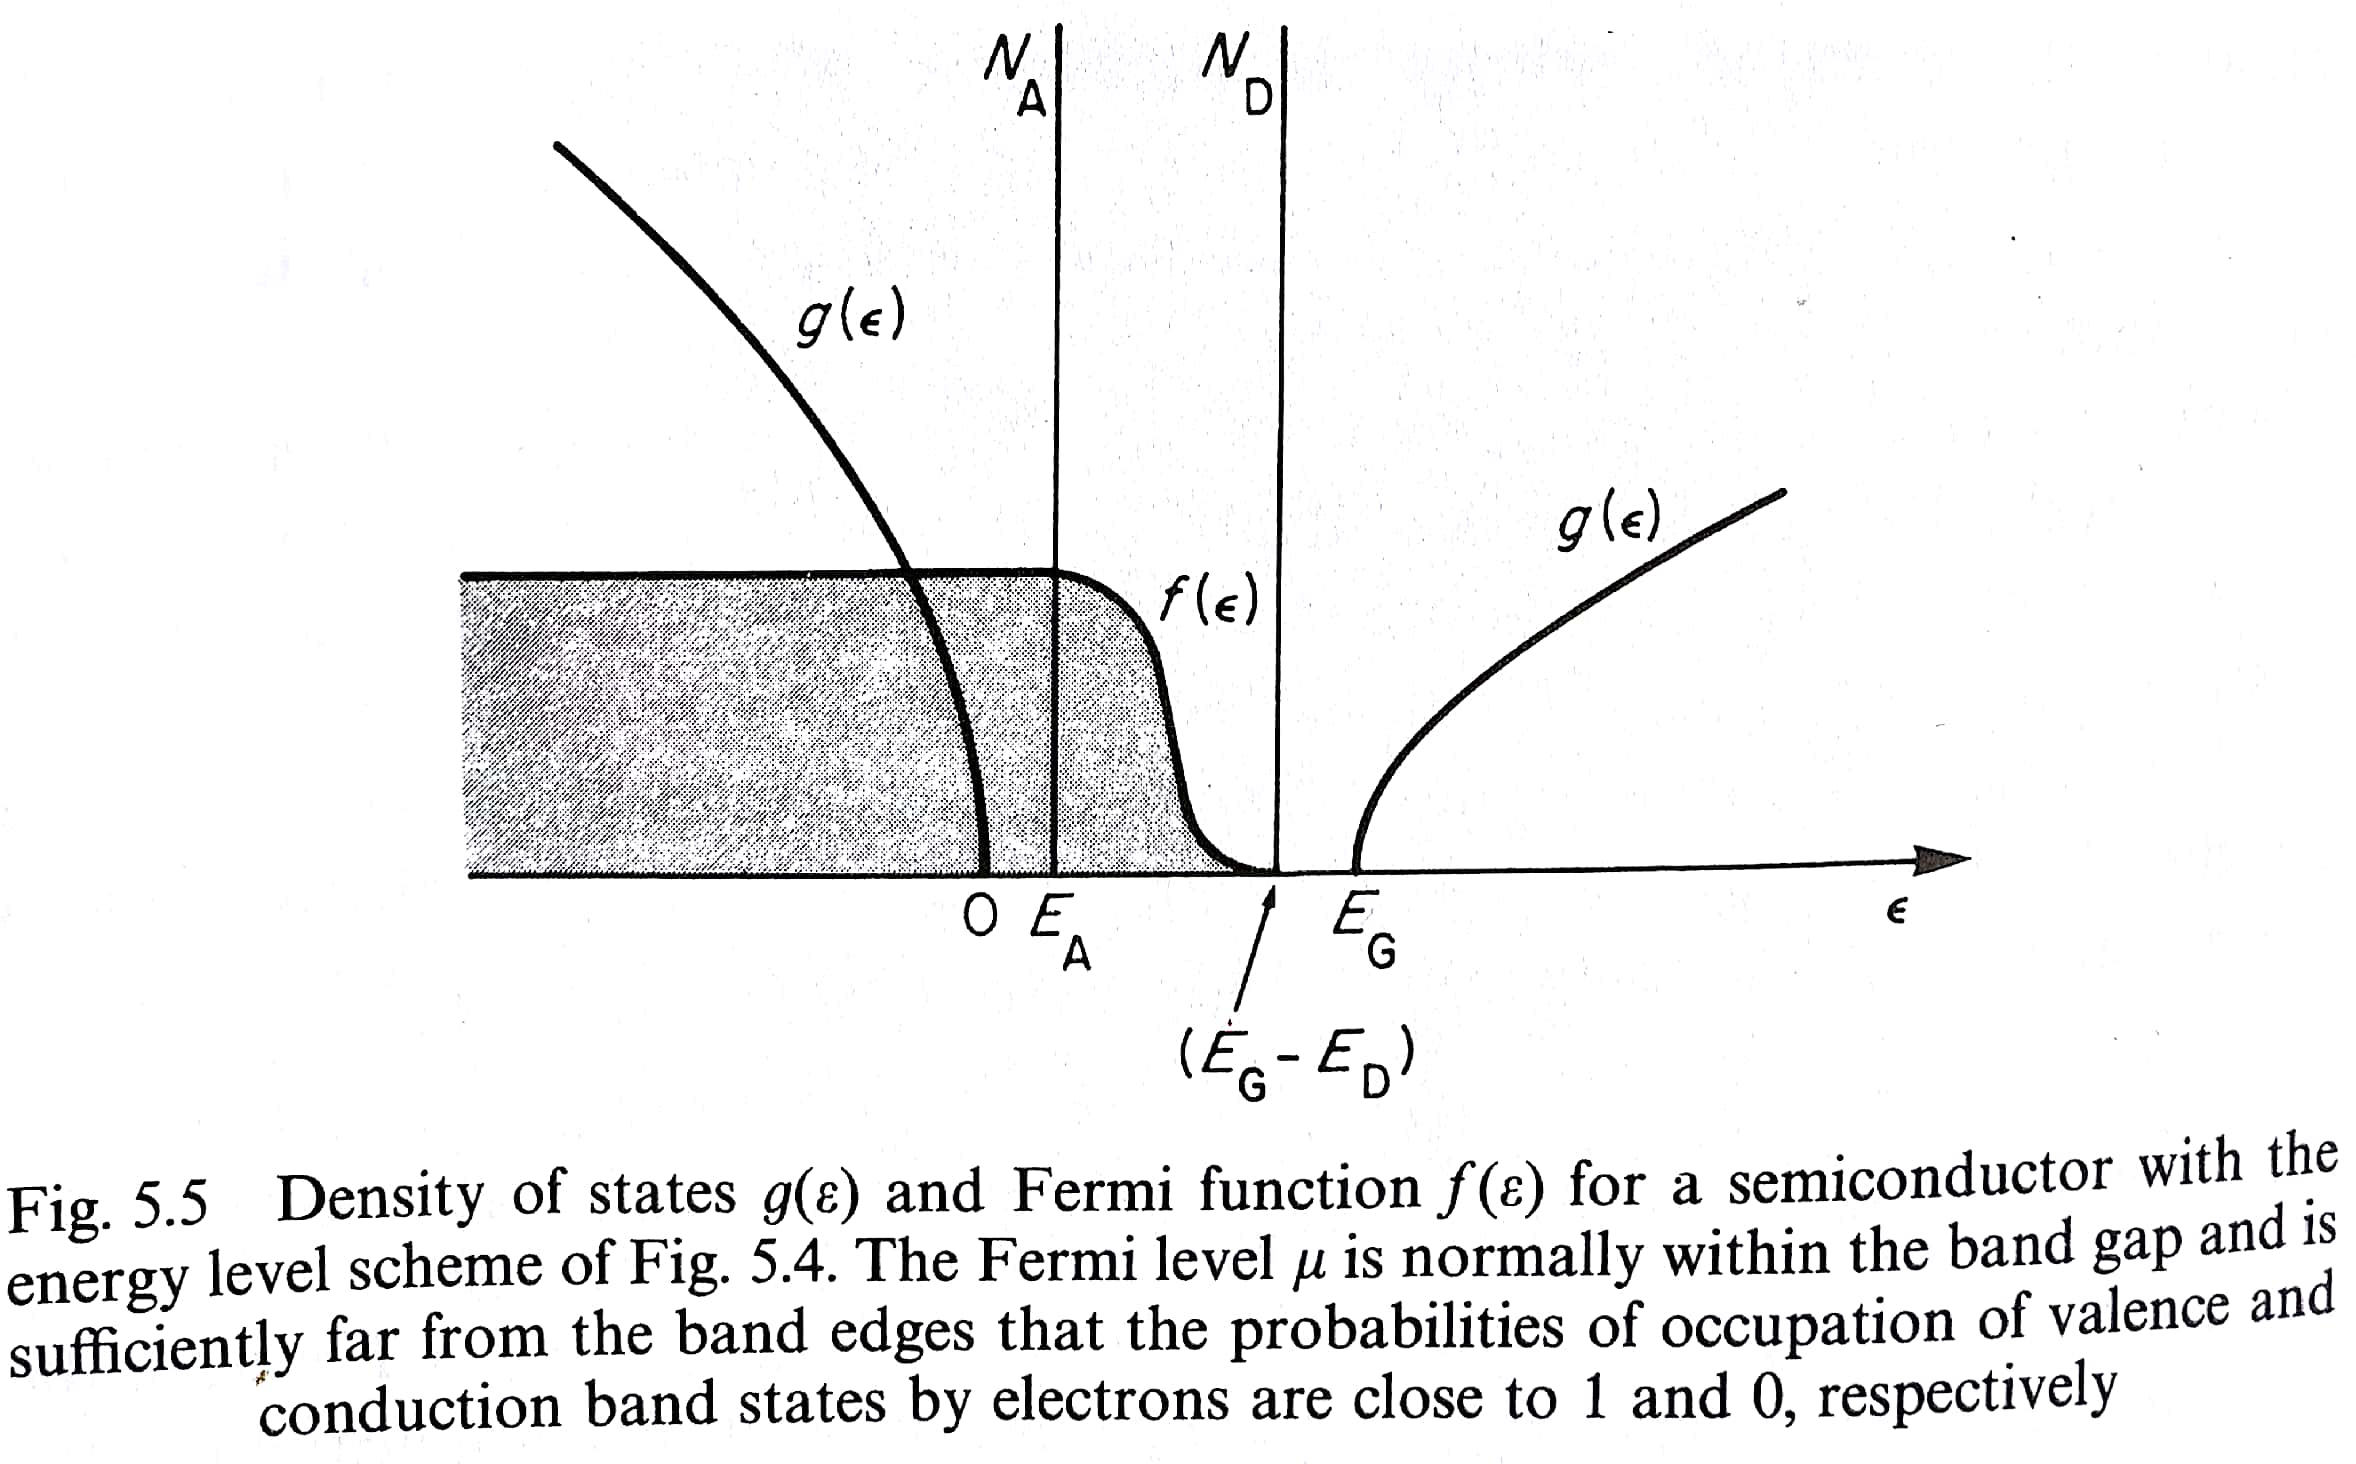
\includegraphics[width=0.7\textwidth]{fermi-level}
	\caption{Copied from Solid State Physics by J.R. Hook and H.E. Hall}
	\label{fig:fermi-level}
\end{figure}

To calculate the probability that a state in the valence band is occupied by a hole is $1-f(\epsilon)$, and doing a similar treatment as for the conduction electrons, keeping in mind the different limits, we get the number of holes per unit volume to be
\begin{equation}
	p = N_v e^{-\mu/k_B T}
	\label{eq:concentration-holes}
\end{equation}
where
\begin{equation}
	N_V = 2(\frac{2\pi m_h k_B T}{h^2})^{3/2}
\end{equation}

It's also worth nothing that the product of the hole concentration and the conduction electron concentration is independent of the chemical potential, i.e.
\begin{equation}
	np = N_c N_v e^{-E_g/k_B T}
	\label{eq:mass-action}
\end{equation}
\subsubsection{Intrinsic behaviour}
In a pure semiconductor, the only holes that can exist is the hole left behind by electrons excited into the conduction band. In other words
\begin{equation}
	n_i = p_i = (N_c N_v)^{1/2} e^{-E_G/2k_BT}
\end{equation}
We have the same concentration of holes as we do of conduction electrons. The subscript $i$ identifies these concentrations as the \textbf{intrinsic carrier concentrations}. Using equations~\ref{eq:concentration-electrons}~\ref{eq:concentration-holes} we can get the chemical potential to be
\begin{equation}
	\mu = \frac{1}{2} E_G + \frac{3}{4} k_B T ln(m_h/m_e)
\end{equation}
and since usually $k_B T \ll E_g$ the Fermi level is normally in the middle of the band gap.
\subsubsection{Extrinsic behaviour}
To find the chemical potential in a semiconductor with acceptor and donors, we require that every negative charge must have a positive charge, thus making the metal electrically neutral. This is something that is obvious when you think of the fact that the material must be electrically neutral when formed, we thus have
\begin{equation}
	n + N^-_A = p + N^+_D
	\label{eq:neutral}
\end{equation}
where $N^-_A$ is the concentration of acceptors and $N^+_D$ is the concentration of donors, given in term of the Fermi function by
\begin{equation}
	N^+_D = N_D [1-f(E_G - E_D)]
\end{equation}
and
\begin{equation}
	N^-_A = N_A f(E_A)
\end{equation}
By inserting the equations~\ref{eq:concentration-electrons}~\ref{eq:concentration-holes} for n and p in equation~\ref{eq:neutral} we can determine $\mu$. This is not possible to do analytically for but a few special limiting cases though.

A common situation is to have impurities of both forms. Lets now assume that we have much more donors then acceptors. Acceptor levels have lower energy, thus they will be filled by electrons from donors at $T=0$. Thus we have $N_D-N_A$ donor levels un-ionized. Due to the Fermi level only being partly occupied at T=0, we have $\mu = E_G - E_D$\footnote{For some reason}. At very low temperatures ($k_B T \ll E_D$), where the number of ionized donors has not changed much, we then have the from equation~\ref{eq:concentration-electrons} that the conduction electron concentration is
\begin{equation}
	n \approx N_C e^{-E_D/k_B T}
\end{equation}
if $k_B T \ll e_D$. Due to the fact that $E_D \ll E_G$ the electron concentration is much greater then for the intrinsic concentration given earlier. But given the law of mass action (eq~\ref{eq:mass-action}), the hole concentration is very much less then its intrinsic value. These kind of materials with lots more electrons in the conduction band then holes in the valence band, are called \textbf{n-type material}, where electrons are called the \textbf{majority carrier} and the holes are the \textbf{minority carrier}. The opposite situation where holes are the majority carrier, are called \textbf{p-type material}. The p-type material at absolute zero has a Fermi level $\mu = E_A$, thus given us the hole concentration
\begin{equation}
	p \approx N_V e^{-E_A/k_B T}
\end{equation}
when $k_B T \ll E_A$. 

But this was at $T=0$! Who da fuck operates on this level anyway? Even in space we have like 2 kelvin at least due to background radiation. So if we look the n-type material, at a temperature where all the donors and acceptors are ionized equation~\ref{eq:neutral} must give us
\begin{equation}
	n = N_D - N_A 
\end{equation}
Thus using equation~\ref{eq:concentration-electrons} with this we get
\begin{equation}
	\mu = E_G - k_B T \ln{(\frac{N_C}{N_D-N_A})}
\end{equation}
And must semiconductors operate on a level where all impurities are ionized at room temperature. But when increasing the temperature further we get that the hole concentration approaches the electron concentration and voila, we have intrinsic behaviour. This transition of behaviour is depicted in figure~\ref{fig:extrinsic}.
\begin{figure}[!ht]
	\centering
	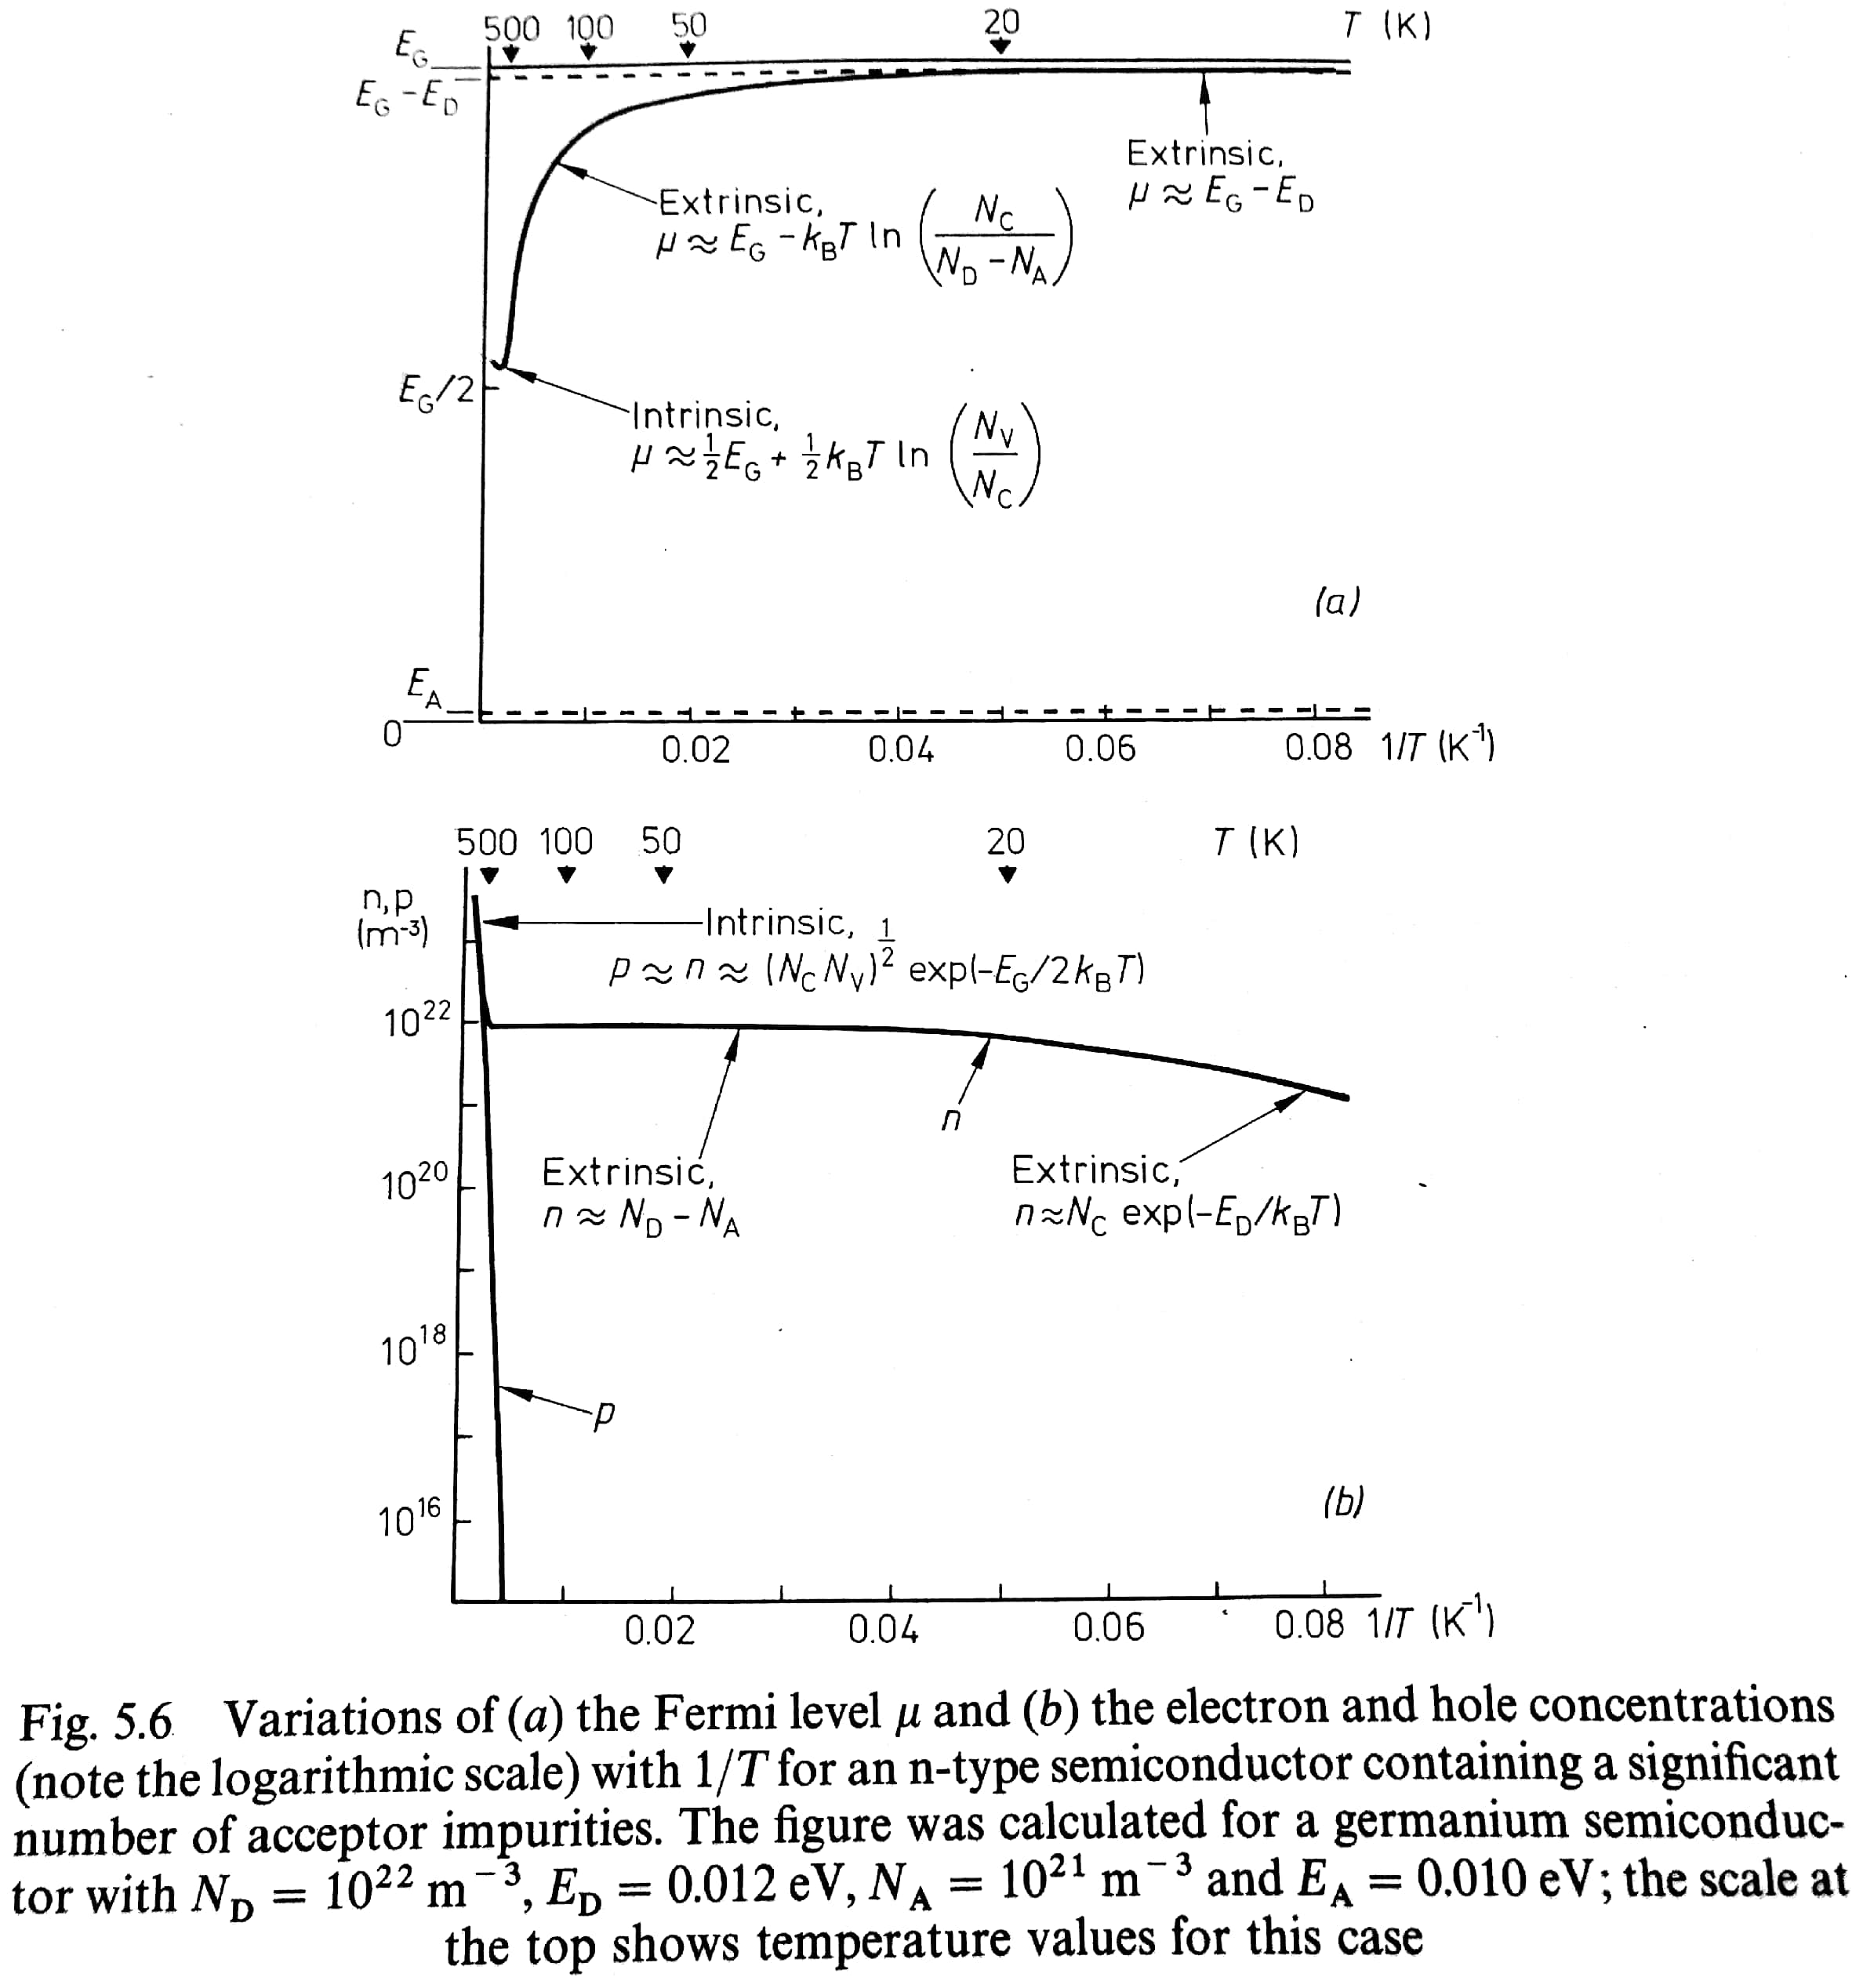
\includegraphics[width=0.7\textwidth]{extrinsic}
	\caption{Copied from Solid State Physics by J.R. Hook and H.E. Hall}
	\label{fig:extrinsic}
\end{figure}

\subsection{Absorption of electromagnetic radiation}
Looking at figure~\ref{fig:absorption} we can see that we have absorption of ems at certain energies. Actually we have two different energies where we have jumps of absorption for germanium. The first one at $T=77k$ seem to occur at about 0.73eV while the second, much steeper increase in absorption, occurs at 0.87eV. Why is this? Why do we seemingly have two energy gaps (The absorption is caused by electrons being excited into the valence band). Well look at figure~\ref{fig:absorption-jump}. The first jump is associated with a energy change \emph{and} momentum change (change in $\pmb{k}$). While the second jump is a straight jump which makes the electrons only change in energy level, but not momentum. 

This momentum is taken from a phonon in the lattice in the beginning, this because a photon cannot carry that much momentum. So electrons which is high up in the valence band can be excited by a smaller energy as long as its momentum changes too. This is a more gradual process since with more energy different amount of momentum changes(from different phonons) is used in the transition. But when the photons have enough energy to create a vertical jump for the electrons across the bands, then we get a much steeper jump in absorption and then it increases linearly, albeit not very steeply. Which seem to concur with how the bands looks.
\begin{figure}[!ht]
	\centering
	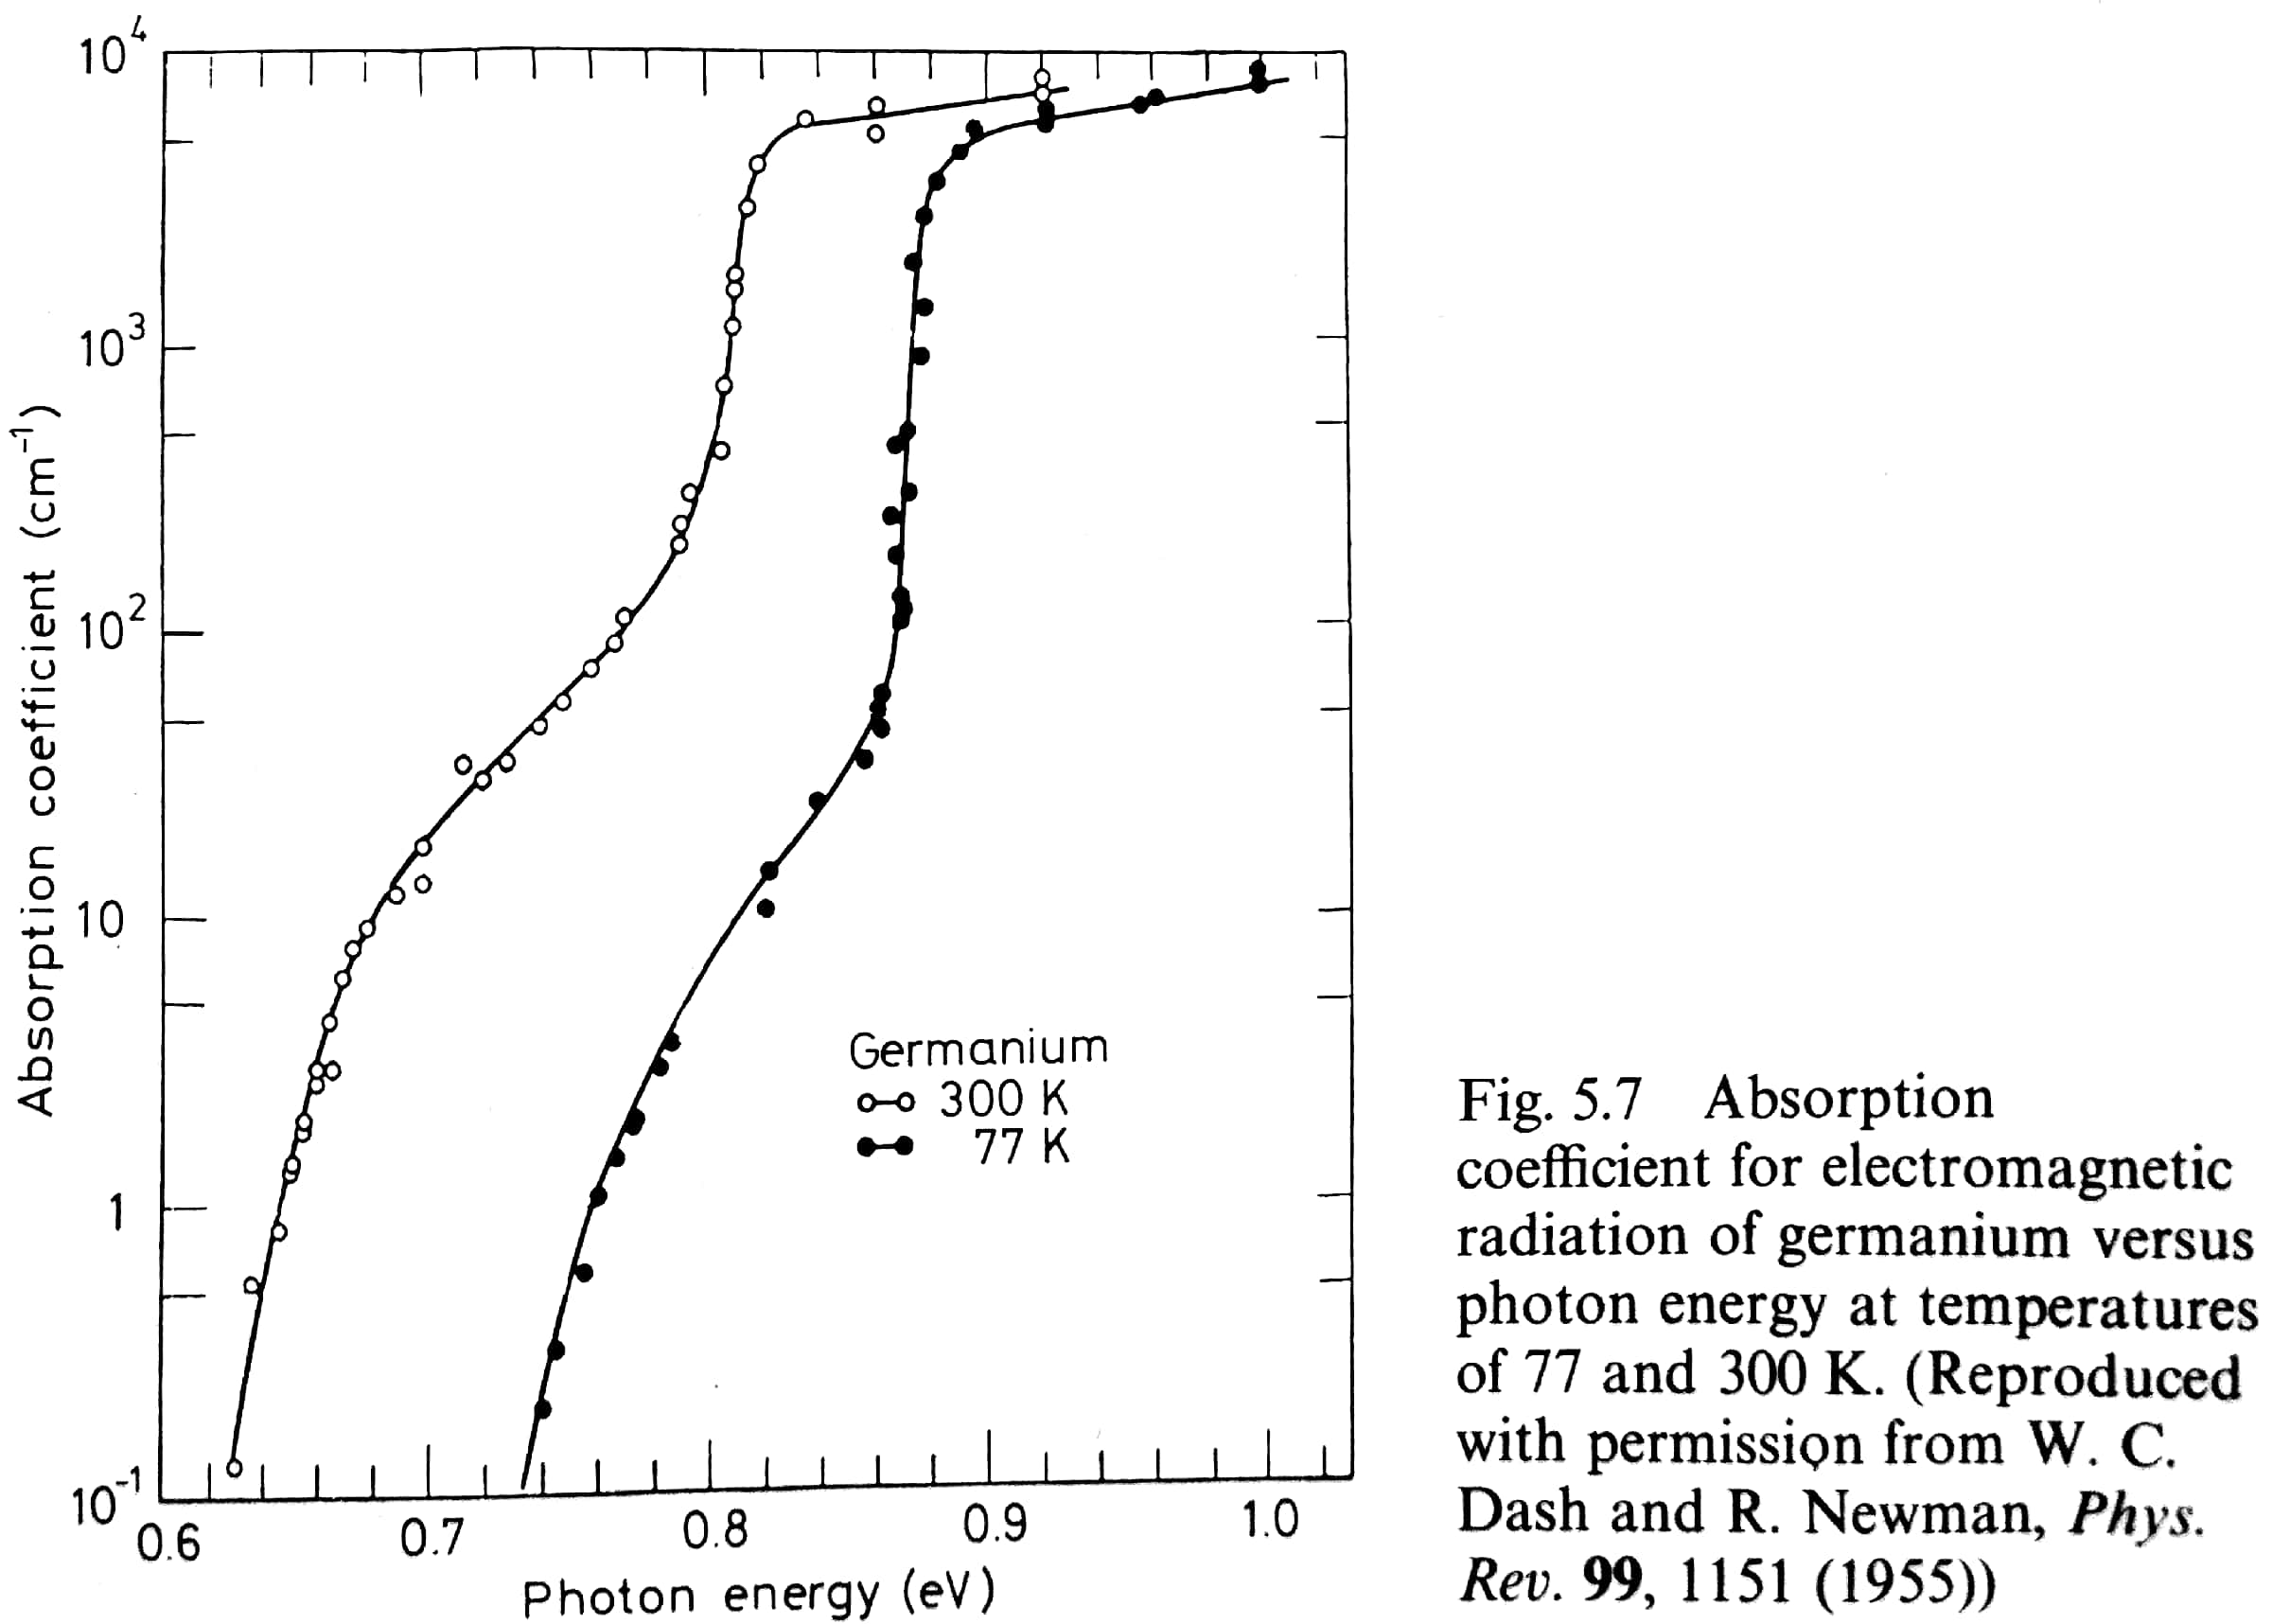
\includegraphics[width=0.7\textwidth]{absorption}
	\caption{Copied from Solid State Physics by J.R. Hook and H.E. Hall}
	\label{fig:absorption}
\end{figure}
\begin{figure}[!ht]
	\centering
	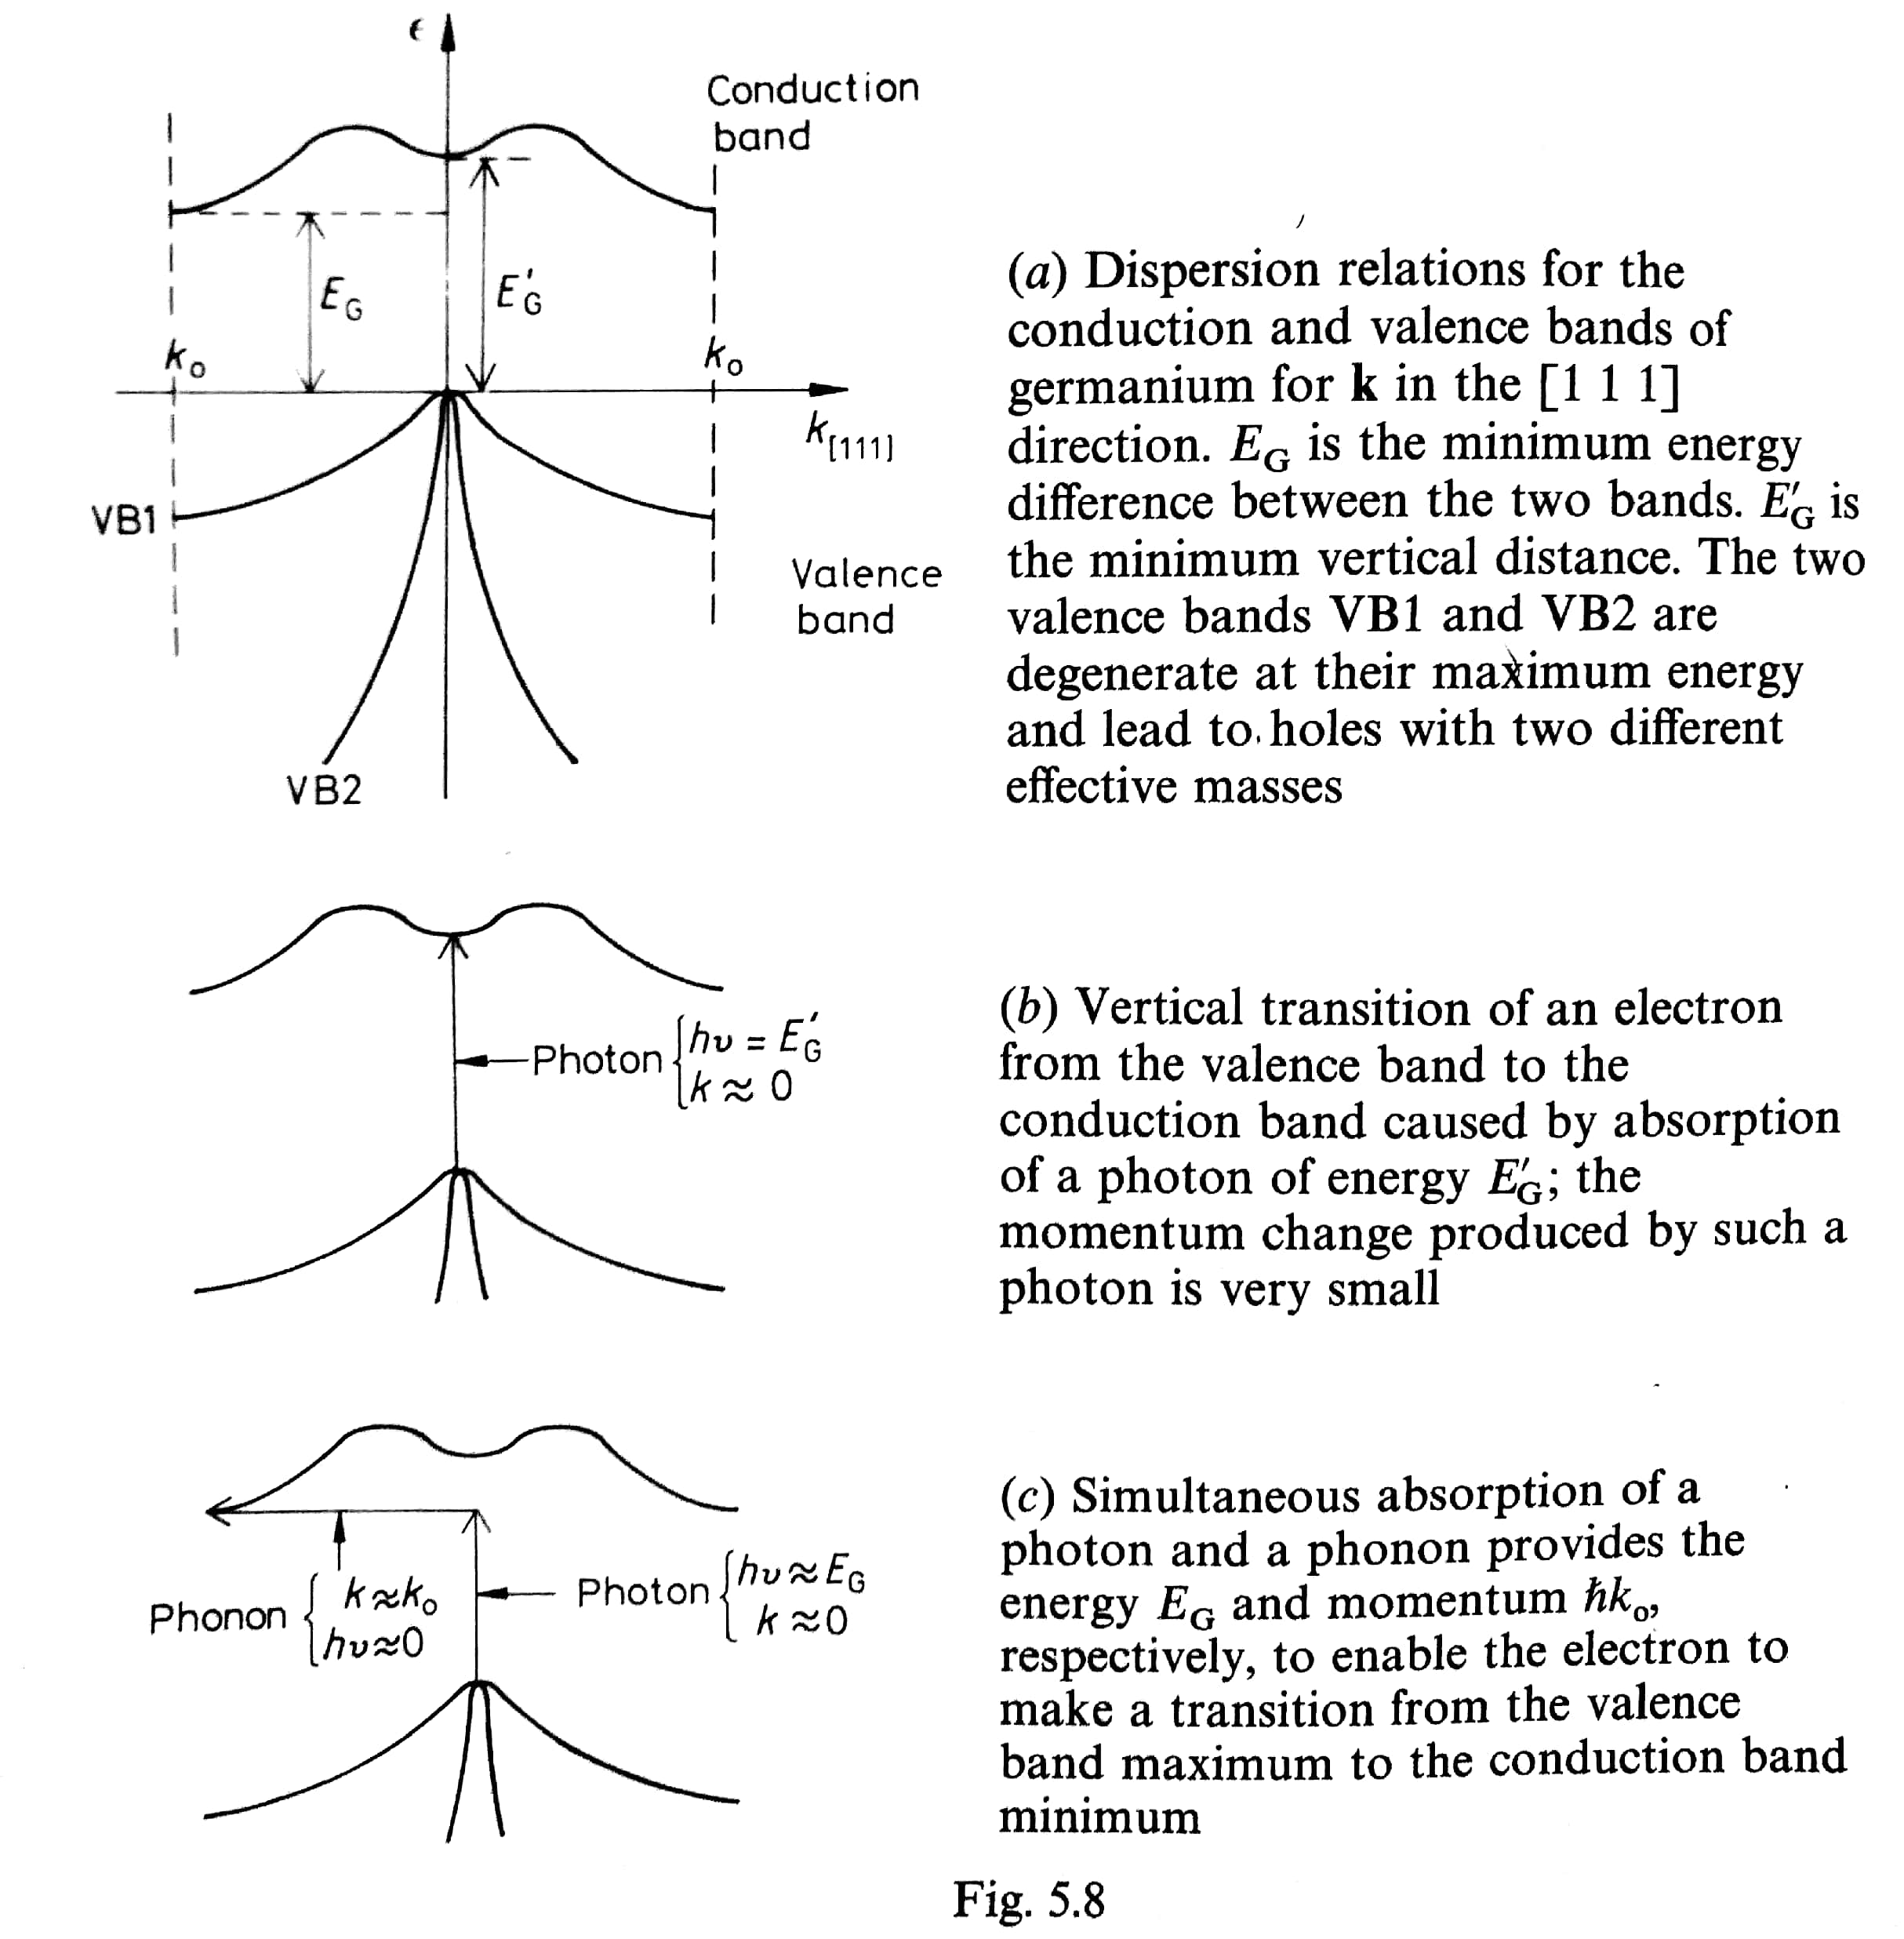
\includegraphics[width=0.7\textwidth]{absorption-jump}
	\caption{Copied from Solid State Physics by J.R. Hook and H.E. Hall}
	\label{fig:absorption-jump}
\end{figure}
\subsection{Transport properties}
To describe the motion of the carriers in the presence of electric and magnetic fields we use these equations (only for reference)
\begin{align}
	m_e (\frac{d\pmb{v}_e}{dt} + \frac{\pmb{v}_e}{\tau_e}) &= -e\pmb{E} - e\pmb{v}_e \times \pmb{B} \\
	m_h (\frac{d\pmb{v}_h}{dt} + \frac{\pmb{v}_h}{\tau_h}) &= e\pmb{E} + e\pmb{v}_h \times \pmb{B} \\
\end{align}
\subsubsection{Electrical conductivity}
When we have only a dc-electric field the equation of motions becomes
\begin{align}
	\pmb{v}_e &= - \mu_e \pmb{E} \\
	\pmb{v}_h &=  \mu_h \pmb{E} 
\end{align}
with
\begin{align}
	\mu_e &= \frac{e\tau_e}{m_e} \\
	\mu_h &= \frac{e\tau_h}{m_h} 
\end{align}
with the resulting current
\begin{equation}
	\pmb{j} = -ne\pmb{v}_e + pe\pmb{v}_h =\ldots= \sigma \pmb{E}
\end{equation}
where 
\begin{equation}
	\sigma = n e \mu_e + p e \mu_h
	\label{eq:conductivity-semiconductor}
\end{equation}
From equation~\ref{eq:conductivity-semiconductor} we can see how the conductivity depends  on the charge carriers through $c$ and $p$. 

This has some interesting effects on the conductivity of a semiconductor. Looking at figure~\ref{fig:semiconductor-conductivity} we can see how the conductivity relates to temperature in different impurity levels. What's mainly effected in our conductivity equation is the collision time at different temperatures.
\begin{figure}[!ht]
	\centering
	\includegraphics[width=0.7\textwidth]{semiconductor-conductivity}
	\caption{Copied from Solid State Physics by J.R. Hook and H.E. Hall}
	\label{fig:semiconductor-conductivity}
\end{figure}
\newpage
\subsubsection{Hall effect}
Basically, if we use the electromagnetic motion equations for charge carriers in semiconductors the hall effect can obtain a positive and negative sign depending on what carrier is the major carrier. If its holes it's positive, if its electrons it's negative.

\section{Superconductivity}
\subsection{Introduction}
Its difficult to measure the resistance in superconductors, since it has none!\footnote{well at least under its critical temperature}. What one do is look at the decay of the current in a loop of superconductors. The current should decay with the time constant
\begin{equation}
	\tau = L/R
\end{equation}
where $L$ is the self-inductance and $R$ is the resistance of the loop. If this is not observed then we see that as superconductivity.
\subsection{Magnetic properties of superconductors}
\subsubsection{Type I superconductors}
There are two classes of superconductors, depending on how the interact with a magnetic field. \textbf{Type I} superconductors has the peculiar effect of being distrusted\footnote{I.e.\ no longer superconductive} by a  modest magnetic field $B_c$, known as the \textbf{Critical field}. \textbf{Type II} superconductors behave differently under a magnetic field, but in this section we will only look at type I superconductors.

$B_c$ as a function of temperature for mercury is seen in figure~\ref{fig:bc}. To a good approximation the temperature dependence of $B_c$ is
\begin{equation}
	B_c(T) = B_c(0) [1-(\frac{T}{T_c})^2].
\end{equation}
Given that there exists a critical field, there  also exists a critical current for flow along a wire, which occurs when the field due to the current equals $B_c$. This is known as \textbf{Silsbee hypothesis}. 
\begin{figure}[!ht]
	\centering
	\includegraphics[width=0.7\textwidth]{bc}
	\caption{Copied from Solid State Physics by J.R. Hook and H.E. Hall}
	\label{fig:bc}
\end{figure}
In figure~\ref{fig:flux-expulsion} we can see the screening known as the \textbf{Meissner effect}. Basically the screening make the superconductor act as a perfect diamagnet opposite to the applied magnetic field under $B_c$. Thus the superconductor has a susceptibility of $\xi = -1$ in this region.
\begin{figure}[!ht]
	\centering
	\includegraphics[width=0.7\textwidth]{flux-expulsion}
	\caption{Copied from Solid State Physics by J.R. Hook and H.E. Hall}
	\label{fig:flux-expulsion}
\end{figure}


\section{Crystal Dynamics - again!}
\subsection{Lattice vibration of one-dimensional crystals}
\subsubsection{chain of two types of atoms}
Read in book at your leisure

\section{Crystal dynamics}
\subsection{Heat capacity from lattice vibrations}
\subsubsection{The density of states}
Periodic boundary condition for one-dimensional crystals yields the possible wavenumbers
\begin{equation}
	k = \frac{2 \pi p}{L}
\end{equation}
where $L = Na$ and $N$ is the number of atoms, $a$ is the interatomic spacing. The k density is can be given in the range $k \to k+dk$ to be
\begin{equation}
	\rho_r(k) dk = \frac{L}{2\pi} dk
\end{equation}
Note here that the integer $p$ can be both positive and negative. This hold for running waves, or periodic boundary conditions on the crystal. I we have fixed boundary condition the normal modes are standing waves, and we have an integral number of half-wavelengths in the chain so $L = n \lambda /2$, $k=2\pi/\lambda = n \pi/L$.  We then get in the range $k \to k +dk$
\begin{equation}
	\rho_s(k) dk  = \frac{L}{\pi} dk
\end{equation}
So we have twice as many normal modes!  But the difference too is only positive integer in the k so we get half again, and voila! The same amount of normal modes.

To find the density of states per unit frequency range $g(\omega)$ we can use $dn$ - number of modes with frequency $\omega \to \omega + d \omega$ corresponding to the range $k \to k + dk$ we have
\begin{equation}
	dn = \rho_s(k) dk = g(\omega) d\omega
\end{equation}
and from this we get
\begin{equation}
	g(\omega) = p_s(k) \frac{dk}{d \omega}.
	\label{eq:states-freq}
\end{equation}
Using a previously obtained result for $\omega(k)$ for the one-dimensional crystal we thus get
\begin{equation}
	g(\omega) = \frac{2N}{\pi} (\frac{4K}{M} - \omega^2)^{-1/2}
\end{equation}
The energy of the lattice vibration is obtained by integrating the energy of a single oscillator(previously derived) of the distribution of vibration frequencies, thus
\begin{equation}
	E = \int^\infty_0 (\frac{1}{2} \hslash \omega + \frac{\hslash \omega}{e^{\hslash \omega/k_B T} - 1}) g(\omega ) d\omega
	\label{eq:vibration-energy}
\end{equation}
Difficult to calculate this integral, but you can do some analysis in some cases, and computers in other. Especially in high or low temperature limits its easier to do an analysis.

In the book we then go over to 2d and 3d crystals. Here i will only give the result.

\paragraph{3d-crystal}
density of k-state
\begin{equation}
	g(k) = \frac{Vk^2}{2\pi^2}
\end{equation}
Density of states per unit frequency range
\begin{equation}
	g(\omega) = g(k)\frac{dk}{d\omega} = \frac{Vk^2}{2\pi^2} \frac{dk}{d\omega}
\end{equation}
But to solve we need to look at limits
\subsubsection{The high and low temperature limits}
At high temperatures we get the heat capacacity
\begin{equation}
	C = 3Nk_B
\end{equation}
If we have a temperature over the characteristic temperature $\Theta = \hslash \omega/k_B$.

For low temperatures we can see $\omega = v_s k$ for long-wavelength acoustic modes. Using this and noting the are two transversal branches and one longitudal branch in three dimensions we can figure out the density of states per unit frequency, but into the integral for the energy and differentiate on $T$ to get the heat capacity 
\begin{equation}
	C = \frac{2V\pi^2 k_B}{15} (\frac{1}{v_L^3} + \frac{2}{v_T^3}) (\frac{k_B T}{\hslash})^3
\end{equation}
Which gives us the empirical dependency on $T^3$ for low temperatures!
\subsubsection{The Debye interpolation scheme}
Intressting chapter which looks at when certain simplications holds.

\subsection{Anharmonic effects}
We have assumed in the one-dimensional case that atoms interact through hooks law (springs). But in reality its lennard jones potential, which has a stronger repelling force when atoms are close then attracting force when they are far away. This only got approximated to hooks through our taylor expansion of the potential. Adding additional terms called \textbf{anhormonic terms} from the approximation gives us insight into things like thermal expansion. 

\subsubsection{Thermal expansion}
The volume coefficient of thermal expansion is defined as
\begin{equation}
	\beta = \frac{1}{V} (\frac{\partial V}{\partial T})_p
\end{equation}
To help the analysis of why $\beta$ vanishes in the harmonic limit we rewrite it as
\begin{equation}
	\beta = \frac{1}{B} (\frac{\partial p}{\partial T})_V
\end{equation}
Where 
\begin{equation}
	B = - V (\frac{\partial p }{\partial V})_T
\end{equation}
We know that $p$ is dependent on helmots free energy through
\begin{equation}
	p = - (\frac{\partial F}{\partial V})_T
\end{equation}
and that in the harmonic approximation we have
\begin{equation}
	F = E_{pot} + F_{modes}
\end{equation}
Where $E_{pot}$ is the temperature independent potential energy associated with the interatomic interactions, and $F_{modes}$ is the free energy associated with the lattice vibrations.  We're given the terms for the energies related to the energy of the lattice vibration in the harmonic level, and see it does not have the volume dependence, thus reducing $p$ to zero. Thus we have no thermal expansion. 

But with the extra anharmonic terms we get the volume dependence and $p$ becomes (if througly calculated)
\begin{equation}
	p = - \frac{d E_{pot}}{dV} - \sum_{modes} \hslash \frac{\partial \omega}{\partial V} (\frac{1}{2} + \frac{1}{e^{\hslash \omega/k_B T)} - 1})
\end{equation}
And through assuming that the volume dependence of all lattice mode frequencies is the same and can be represented by the simple power law $\omega \propto V^{-\gamma}$ we get
\begin{equation}
p = - \frac{dE_{pot}}{dV} + \frac{\gamma E_{modes}}{V}
\end{equation}
This gives us a $\beta$ of
\begin{equation}
	\beta = \frac{\gamma C_V}{BV}
\end{equation}
Thus the expansion relates directly to how the heat capacity changes with temperature.


\section{Waves in crystals}
\subsection{Normal modes and the reciprocal lattice}
\subsubsection{Brillouin zones and the plotting of dispersion relations}
When looking at one-dimensional electron dispersion relations we found it useful to split $\pmb{k}$-space into Brillouin zones at the $k$ values for which Bragg diffraction of the electron waves occurred. This diffraction creates standing waves instead of running waves at the zone boundaries. The energy gaps that occur under the periodic potential also happen to exists on the Brillouin zones. In a one-dimensional crystal the boundaries of the $n$th are given in terms of the lattice spacing $a$ through
\begin{equation}
	(n-1)\pi/a < |k| < n \pi / a
\end{equation}	
And each zones occurs two times, symmetrically around the origin. 

If we use a more general diffraction rule as that one given earlier in section~\ref{sec:dispersion}. Using this and some simplification we can generalize using vectors and we get $\pmb{k}$ for an incoming wave must satisfy
\begin{equation}
	2\pmb{k} \cdot \pmb{G} = G^2
\end{equation}
where $\pmb{G}$ is any vector of the reciprocal lattice. 

\begin{figure}[!ht]
	\centering
	\includegraphics[width=0.7\textwidth]{geo-int}
	\caption{Copied from Solid State Physics by J.R. Hook and H.E. Hall}
	\label{fig:geo-int}
\end{figure}

\begin{figure}[!ht]
	\centering
	\includegraphics[width=0.7\textwidth]{brillouin-2d}
	\caption{Copied from Solid State Physics by J.R. Hook and H.E. Hall}
	\label{fig:brillouin-2d}
\end{figure}

\begin{figure}[!ht]
	\centering
	\includegraphics[width=0.7\textwidth]{brillouin-weigner}
	\caption{Copied from Solid State Physics by J.R. Hook and H.E. Hall}
	\label{fig:brillouin-weigner}
\end{figure}

\newpage












%\begin{thebibliography}{9}
%\end{thebibliography}
\clearpage
\appendix
\section{Appendix}

\end{document}

